% Plain-language review document (explaneat plain-language review), v5.
\documentclass[a4paper,10pt]{article}
\usepackage[margin=1.8cm]{geometry}
\usepackage{amsmath}
\usepackage{amssymb}
\usepackage{booktabs}
\usepackage{tabularx}
\usepackage{graphicx}
\usepackage[table,usenames,dvipsnames]{xcolor}
\usepackage{tikz}
\usetikzlibrary{arrows.meta,fit,backgrounds,positioning,calc}
\usetikzlibrary{shapes.geometric}
\usepackage{longtable}
\usepackage{pdflscape}
\usepackage{float}
\usepackage[font=small,labelfont=bf]{caption}
\usepackage{array}
\usepackage[unicode=true,hidelinks]{hyperref}
\setcounter{tocdepth}{3}
\setcounter{secnumdepth}{3}
% Review markers, copied from dissertation.tex (7 Nov 2026) for standalone builds.
\newif\ifreviewmarks
\reviewmarkstrue
\newcommand{\reviewrule}{\noindent{\color{BrickRed}\rule{\linewidth}{0.8pt}}}
\newenvironment{drafted}[1][]{%
  \ifreviewmarks\par\addvspace{\medskipamount}\reviewrule\par\nopagebreak
  \noindent{\color{BrickRed}\sffamily\footnotesize\textbf{Thesis Draft}\quad #1\hfill review}\par\nopagebreak\smallskip\fi}{%
  \ifreviewmarks\par\smallskip\noindent{\color{BrickRed}\sffamily\footnotesize end of thesis draft}\par\nopagebreak\reviewrule\par\medskip\fi}
\newcommand{\figreview}[1]{\ifreviewmarks\par\smallskip{\color{NavyBlue}\sffamily\footnotesize\textbf{Figure note:} #1}\par\fi}
\begin{document}
\begin{center}{\Large\bfseries Plain-language explanation: churn100-s4-c3\par}\vspace{2mm}{\small AI-assisted drafts for review. Nothing here has been verified by a person.\par}\end{center}
\noindent\textbf{How to read this.} Explanations are built up but read down: the summary first, then each part from the whole model down, in plain words, each sentence followed by the claims it rests on (C01, C02, \ldots; every cited claim was computed on the model and checked). Numbers are changes in predicted risk for a typical patient. The technical record (original hypotheses, formulas, evidence tables with the test check, ranges and n) is at the end. The text describes what the model does, not the world; whether it is plausible is for the reviewer to judge.
\par\medskip\noindent\textbf{What changed in v5e (figures).} v5e: every diagram is a numbered figure with a caption (list of figures after the contents) and the text refers to it; the whole-network figure has its own landscape page, scaled to the page, with a short caption and its description in the text; an input used by several parts is drawn under each of them (same input, repeated for readability, dotted outline); and an appendix figure shows the trained network before any explanation (no parts, no splits).
\par\medskip\noindent\textbf{What changed in v5c (tables and diagrams).} v5c: the evidence tables are landscape, compact and shaded by row, with the header repeated on every page (longtable and pdflscape, used in this review PDF only; the thesis preamble has neither). In the diagrams each input is drawn once, in a shared row along the bottom (the explanation's split copies of an input are listed in the technical detail instead), every cluster has one output rectangle with its plain name, the inputs that feed the output directly meet in a drawn 'sum', and a one-line legend explains the edges.
\par\medskip\noindent\textbf{What changed in v5b (diagrams).} v5b uses one grouping everywhere, the annotation hierarchy: the summary's diagram is the same picture as the whole model's section, and a part that is itself a weighted sum (blood pressure with cholesterol) is a part of its own, described as one that adds up, so the text counts three parts throughout; the lint checks every 'N parts' against the hierarchy. A full-structure diagram follows the summary: every node and connection, nested by part, with the inputs that feed the output directly in their own cluster and the unused input columns listed. Each section from the top down adds its own region of that diagram, with stubs for connections from or to other parts; each connection is drawn in exactly one section. The gate's text now says that it lowers the risk for the patients it acts on, and that more vessels and higher cholesterol take that lowering away; its vessel statements are one per group.
\par\medskip\noindent\textbf{What changed in v5 (read down).} v5 reads the explanation down. The summary (one line, a diagram, one paragraph per block) is as in v4, except that the paragraph on what adds up is split into protective items, risk-raising items and rare results, and an input that also feeds a part is quoted with its direct contribution only (the rest is in that part's paragraph). Then the document walks the annotation hierarchy from the whole model down: for each part a plain hypothesis (what it does for the prediction), plain evidence (what was checked and what it showed; for a part made of others, what they are and how they combine), a diagram one level down and where to read on. The original hypotheses, closed forms and evidence tables are in 'Technical detail' at the end. Statements about structure (what a part is made of, a copy of another part, a formula that reproduces it) are now claims of their own, checked on the graph and the data.
\par\medskip\noindent\textbf{v4.} v4 follows the structure of the explanation. The summary opens with one line and a diagram at the same grouping, then gives one paragraph per top-level block of the annotation hierarchy: one for everything that adds up independently (the inputs that feed the model score directly, and parts that are a weighted sum), and one for each part that combines its inputs in another way: what it combines, how, and for whom. 'Parts in detail' follows the hierarchy below that, with a diagram one level down for each part that contains others. The prose no longer says 'clearly', 'slightly', 'consistently' or 'on the training data only': the numbers carry it, and the test check, the ranges and n stay in the evidence tables. Only genuinely small groups are marked, with their n. The lint rejects the confidence words and checks the block structure.
\tableofcontents
\listoffigures
\clearpage
\begin{drafted}[plain-language layer: churn100-s4-c3]
\section{churn100-s4-c3}
\noindent{\small Genome \texttt{27f540ac-6acb-4d58-9972-cd71fae31cf0}, explanation \texttt{ffdb207f-1e0f-4d2e-a330-f47b1ca75c4a}. Split: train primary (n=4000), test as a check (n=1000). Claims: 123, verified 121, not supported 2.\par}
\noindent{\small\textcolor{BrickRed}{AI-assisted draft for review (unverified)}\par}\smallskip
\noindent{\footnotesize Reference (typical) customer: the typical customer: the median training customer for every number and the most common training category for every category (not a real customer). account length: 100; area code: area code 415; international plan: no international plan; number customer service calls: 1 calls; number vmail messages: 0 messages; state: West Virginia; total day calls: 100 calls; total day charge: 30.69 US dollars; total day minutes: 180 minutes; total eve calls: 100 calls; total eve charge: 17.12 US dollars; total eve minutes: 201 minutes; total intl calls: 4 calls; total intl charge: 2.78 US dollars; total intl minutes: 10 minutes; total night calls: 100 calls; total night charge: 9.02 US dollars; total night minutes: 200 minutes; voice mail plan: no voice-mail plan. Predicted chance that a customer leaves: 1\%.\par}
\subsection{Summary}
\noindent For a typical customer (in West Virginia, area code 415, no international or voice-mail plan, no voice-mail messages, 1 call to customer service and median usage) the model predicts a chance of leaving of about 1\%; it adds up four parts: fixed-weight inputs, service calls, heavy daytime use and state units.\,{\scriptsize\textcolor{NavyBlue}{[C054]}} Figure~\ref{fig:churn100s4c3:summary} shows the model at this level: one box per paragraph below.
\par\medskip\noindent\fbox{\begin{minipage}{0.96\linewidth}\small\textbf{How to read the diagrams.} Edge colour is the sign of that one connection: blue positive, red negative; thicker is a larger weight. The outline and arrow on an input (and on a part's output box) is its overall effect on the final prediction, read from the verified claims: orange and up arrow raises it, teal and down arrow lowers it, grey and double arrow depends (it goes both ways, or differs between levels). A negative connection into a part that itself raises the prediction means that input lowers the prediction; through a hinge the overall effect can only be read from the claims, not from the edges. Up arrow means towards churn; down arrow, away from it. A double outline marks an input (or a part's output) that acts at a fixed rate everywhere: it adds the same amount to the score per unit, so it is explained by its rate alone (see 'Linear factors'); a dashed double outline, at a fixed rate on the observed data. The normal outline is an input whose effect switches on and off somewhere. For example, a voice-mail plan has a negative connection into 'Fixed-weight inputs', a part that raises the predicted chance that a customer leaves, so a voice-mail plan lowers it.\end{minipage}}\par\medskip
\begin{figure}[H]\centering
\resizebox{!}{\ifdim\height>0.5\textheight 0.5\textheight\else\height\fi}{%
\resizebox{\ifdim\width>\linewidth\linewidth\else\width\fi}{!}{%
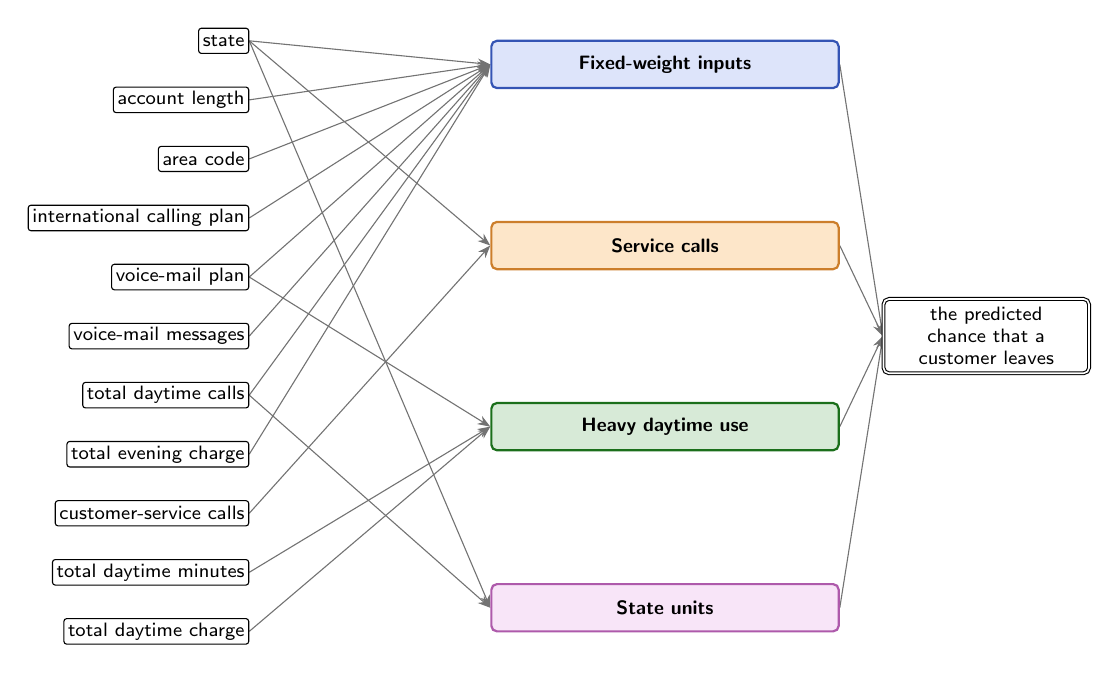
\begin{tikzpicture}[
  font=\sffamily\scriptsize, >={Stealth[length=1.6mm]},
  inp/.style={draw, rounded corners=1pt, fill=white, inner sep=1.5pt, minimum height=3.2mm, anchor=east},
  abox/.style={draw, thick, rounded corners=2pt, align=center, inner sep=3pt, minimum height=6mm, text width=42mm},
  outp/.style={draw, double, rounded corners=2pt, fill=white, align=center, inner sep=3pt, text width=24mm},
  agg/.style={draw=black!55},
]
\node[inp] (i0) at (0,3.75) {state};
\node[inp] (i1) at (0,3.0) {account length};
\node[inp] (i2) at (0,2.25) {area code};
\node[inp] (i3) at (0,1.5) {international calling plan};
\node[inp] (i4) at (0,0.75) {voice-mail plan};
\node[inp] (i5) at (0,-0.0) {voice-mail messages};
\node[inp] (i6) at (0,-0.75) {total daytime calls};
\node[inp] (i7) at (0,-1.5) {total evening charge};
\node[inp] (i8) at (0,-2.25) {customer-service calls};
\node[inp] (i9) at (0,-3.0) {total daytime minutes};
\node[inp] (i10) at (0,-3.75) {total daytime charge};
\node[abox, fill=RoyalBlue!18, draw=RoyalBlue!80!black] (b0) at (5.28,3.45) {\textbf{Fixed-weight inputs}};
\node[abox, fill=BurntOrange!18, draw=BurntOrange!80!black] (b1) at (5.28,1.15) {\textbf{Service calls}};
\node[abox, fill=ForestGreen!18, draw=ForestGreen!80!black] (b2) at (5.28,-1.15) {\textbf{Heavy daytime use}};
\node[abox, fill=Orchid!18, draw=Orchid!80!black] (b3) at (5.28,-3.45) {\textbf{State units}};
\node[outp] (out) at (9.36,0) {the predicted chance that a customer leaves};
\begin{scope}[on background layer]
\draw[->, agg, thin] (i0.east) -- (b0.west);
\draw[->, agg, thin] (i1.east) -- (b0.west);
\draw[->, agg, thin] (i2.east) -- (b0.west);
\draw[->, agg, thin] (i3.east) -- (b0.west);
\draw[->, agg, thin] (i4.east) -- (b0.west);
\draw[->, agg, thin] (i5.east) -- (b0.west);
\draw[->, agg, thin] (i6.east) -- (b0.west);
\draw[->, agg, thin] (i7.east) -- (b0.west);
\draw[->, agg] (b0.east) -- (out.west);
\draw[->, agg, thin] (i0.east) -- (b1.west);
\draw[->, agg, thin] (i8.east) -- (b1.west);
\draw[->, agg] (b1.east) -- (out.west);
\draw[->, agg, thin] (i4.east) -- (b2.west);
\draw[->, agg, thin] (i9.east) -- (b2.west);
\draw[->, agg, thin] (i10.east) -- (b2.west);
\draw[->, agg] (b2.east) -- (out.west);
\draw[->, agg, thin] (i0.east) -- (b3.west);
\draw[->, agg, thin] (i6.east) -- (b3.west);
\draw[->, agg] (b3.east) -- (out.west);
\end{scope}
\end{tikzpicture}}}%
\caption{The model at the level of the summary: one box per part.}
\label{fig:churn100s4c3:summary}
\end{figure}
\paragraph{Fixed-weight inputs.} This part adds up most inputs with fixed weights: an international plan raises a typical customer's chance of leaving from about 1\% to about 18\%, and a voice-mail plan lowers it to below 1\%.\,{\scriptsize\textcolor{NavyBlue}{[C055, C063]}} More voice-mail messages raise it steadily, from about 1\% at 0 to about 6\% at 32 messages, flattening out near the bottom because the predicted chance cannot go much lower.\,{\scriptsize\textcolor{NavyBlue}{[C056]}} A higher evening charge also raises it steadily, from about 1\% at 11.76 US dollars to about 2\% at 22.57 US dollars, flattening out near the bottom because the predicted chance cannot go much lower.\,{\scriptsize\textcolor{NavyBlue}{[C059]}} Through it, the state moves the chance from about 1\% in West Virginia to about 5\% in Washington and about 4\% in Nevada, and to below 1\% in Rhode Island, Hawaii and Vermont (72 to 82 training customers per state).\,{\scriptsize\textcolor{NavyBlue}{[C057, C058, C061, C062, C064]}}
\paragraph{Service calls.} This part adds up two parts: an early rise and a late rise in calls to customer service.\,{\scriptsize\textcolor{NavyBlue}{[C090]}} From about 3 calls upwards it adds to the chance slowly at first, then faster: for a typical such customer, 4 calls take it from about 1\% to about 10\%, flattening out near the bottom because the predicted chance cannot go much lower.\,{\scriptsize\textcolor{NavyBlue}{[C089]}} Up to 3 calls the chance rises slowly at first, then faster, from about 1\% to about 2\% for a typical customer, flattening out near the bottom because the predicted chance cannot go much lower.\,{\scriptsize\textcolor{NavyBlue}{[C084]}} That early rise happens only outside Nebraska, California and Colorado: in Nebraska the chance stays at about 1\% from 0 to 3 calls, against a rise from about 1\% to about 2\% elsewhere, slowly at first, then faster, flattening out near the bottom because the predicted chance cannot go much lower.\,{\scriptsize\textcolor{NavyBlue}{[C088]}}
\paragraph{Heavy daytime use.} Daytime minutes add to the chance only once they rise above about 209 minutes, in an uneven way: for a typical such customer, from about 1\% at 0 minutes to about 16\% at 271 minutes, flattening out near the bottom because the predicted chance cannot go much lower.\,{\scriptsize\textcolor{NavyBlue}{[C100]}} The rise is much larger without a voice-mail plan: from 112 to 249 daytime minutes the chance goes from about 1\% to about 6\% without one, but stays below 1\% with one, in an uneven way, flattening out near the bottom because the predicted chance cannot go much lower.\,{\scriptsize\textcolor{NavyBlue}{[C099]}} This part acts on 1074 of 4000 training customers, 290 of whom left; for the typical customer it acts on, the chance is about 1\% without it and about 4\% with it.\,{\scriptsize\textcolor{NavyBlue}{[C102]}}
\paragraph{State units.} This part reads only the state: it raises a typical customer's chance from about 1\% to about 12\% in Rhode Island, to about 3\% in Vermont and to about 2\% in Tennessee.\,{\scriptsize\textcolor{NavyBlue}{[C104, C105, C106]}} It lowers the chance to below 1\% in Virginia and in Nevada.\,{\scriptsize\textcolor{NavyBlue}{[C107, C108]}}
\paragraph{The whole network.} Figure~\ref{fig:churn100s4c3:overview} (next page, landscape) draws every unit and connection of the explained model, nested by part: shaded clusters are the parts of the model and darker boxes the parts inside them; circles are hidden units (h1, h2, \ldots); each cluster's rectangle is its output, and a dashed `sum' stands for an addition the next unit does (drawn, not a unit of the model); the hexagon is the model's output. An input used by several parts is drawn under each of them (same label, dotted outline, the first copy marked with the number of copies): it is the same input, repeated for readability. Not used by the model (input columns with no connection): state: 20 of 51 levels, area code 408, area code 510, total evening minutes, total evening calls, total night-time minutes, total night-time calls, total night-time charge, total international minutes, total international calls, total international charge.
\begin{landscape}
\begin{figure}[p]\centering
\resizebox{\linewidth}{!}{%
\definecolor{netup}{HTML}{D95F02}\definecolor{netdown}{HTML}{1B9E77}\definecolor{netmixed}{HTML}{7F7F7F}%
\begin{tikzpicture}[
  font=\sffamily\scriptsize, >={Stealth[length=1.4mm]},
  inp/.style={draw, circle, fill=white, minimum size=3.2mm, inner sep=0pt},
  hid/.style={draw, circle, fill=white, minimum size=5.2mm, inner sep=0.5pt, font=\sffamily\tiny},
  exitbox/.style={draw, thick, rectangle, fill=white, align=center, text width=17mm, minimum height=5mm, inner sep=1.5pt, font=\sffamily\tiny},
  sumbox/.style={draw, thick, dashed, rectangle, fill=white, align=center, text width=17mm, minimum height=5mm, inner sep=1.5pt, font=\sffamily\tiny},
  outp/.style={draw, thick, regular polygon, regular polygon sides=6, fill=white, minimum size=10mm, inner sep=0pt, font=\sffamily\tiny, align=center},
  stub/.style={draw, dashed, rounded corners=2pt, fill=white, align=center, inner sep=2pt, font=\sffamily\tiny, text width=15mm},
  inlab/.style={font=\sffamily\tiny, align=center, text width=15mm, inner sep=1pt, fill=white, fill opacity=0.8, text opacity=1},
  wpos/.style={draw=NavyBlue}, wneg/.style={draw=BrickRed}, wagg/.style={draw=black!45, line width=1.2pt},
  wmix/.style={draw=Plum},
]
\node[outp] (n0) at (22.99,6.15) {churn};
\node[hid] (n10131) at (25.49,1.9) {h13};
\node[hid] (n11361) at (31.58,1.9) {h14};
\node[hid] (n12374) at (17.67,1.9) {h15};
\node[hid] (n12690) at (33.08,1.9) {h16};
\node[hid] (n1295) at (34.58,1.9) {h2};
\node[hid] (n13068) at (36.08,1.9) {h17};
\node[hid] (n1390) at (37.58,1.9) {h3};
\node[hid] (n15362) at (39.08,1.9) {h18};
\node[hid] (n15490) at (40.58,1.9) {h19};
\node[hid] (n15904) at (36.83,3.25) {h20};
\node[hid] (n17102) at (42.08,1.9) {h21};
\node[hid] (n3118) at (26.99,1.9) {h4};
\node[hid] (n349) at (19.17,1.9) {h1};
\node[hid] (n4000) at (28.49,1.9) {h5};
\node[hid] (n5268) at (18.42,3.25) {h6};
\node[hid] (n5533) at (38.33,3.25) {h7};
\node[hid] (n5786) at (43.58,1.9) {h8};
\node[hid] (n6713) at (14.665,3.25) {h9};
\node[hid] (n7872) at (39.83,3.25) {h10};
\node[hid] (n9436) at (14.665,1.9) {h11};
\node[hid] (n9954) at (45.08,1.9) {h12};
\node[exitbox] (nidentityxlin) at (5.85,1.9) {Fixed-weight inputs $\uparrow$};
\node[exitbox] (nidentityxsvc) at (21.75,4.6) {Service calls $\uparrow$};
\node[sumbox] (ncsumxxannx85) at (26.99,3.25) {sum: Heavy daytime use $\uparrow$};
\node[sumbox] (ncsumxxannx86) at (38.33,4.6) {sum: State units $\updownarrow$};
\node[inp, densely dotted, thick, draw=netmixed, very thick] (ngrpxxstatexxannx87) at (17.095,0.0) {};
\path (ngrpxxstatexxannx87.south) node[inlab, anchor=north] (labngrpxxstatexxannx87) {state (31 of 51 used) ($\times$3) $\updownarrow$};
\node[inp, densely dotted, thick, draw=netmixed, very thick] (ngrpxxstatexxannx86) at (37.43,0.0) {};
\path (ngrpxxstatexxannx86.south) node[inlab, anchor=north] (labngrpxxstatexxannx86) {state (31 of 51 used) $\updownarrow$};
\node[inp, draw=netup, very thick] (ninxxtotalxdayxminutesxxannx85) at (28.79,0.0) {};
\path (ninxxtotalxdayxminutesxxannx85.south) node[inlab, anchor=north] (labninxxtotalxdayxminutesxxannx85) {total daytime minutes $\uparrow$};
\node[inp] (ninxxtotalxdayxchargexxannx85) at (26.99,0.0) {};
\path (ninxxtotalxdayxchargexxannx85.south) node[inlab, anchor=north] (labninxxtotalxdayxchargexxannx85) {total daytime charge};
\node[inp, draw=netup, very thick] (ninxxnumberxcustomerxservicexcallsxxannx87) at (18.895,0.0) {};
\path (ninxxnumberxcustomerxservicexcallsxxannx87.south) node[inlab, anchor=north] (labninxxnumberxcustomerxservicexcallsxxannx87) {customer-service calls $\uparrow$};
\node[inp, densely dotted, thick, draw=netup, very thick] (ninxxtotalxdayxcallsxxannx86) at (39.23,0.0) {};
\path (ninxxtotalxdayxcallsxxannx86.south) node[inlab, anchor=north] (labninxxtotalxdayxcallsxxannx86) {total daytime calls ($\times$2) $\uparrow$};
\node[inp, densely dotted, thick, draw=netdown, very thick] (ninxxvoicexmailxplanxxannx85) at (25.19,0.0) {};
\path (ninxxvoicexmailxplanxxannx85.south) node[inlab, anchor=north] (labninxxvoicexmailxplanxxannx85) {a voice-mail plan ($\times$2) $\downarrow$};
\node[inp, densely dotted, thick, draw=netmixed, very thick] (ngrpxxstatexxannx82) at (4.5,0.0) {};
\path (ngrpxxstatexxannx82.south) node[inlab, anchor=north] (labngrpxxstatexxannx82) {state (31 of 51 used) $\updownarrow$};
\node[inp, draw=netup, very thick] (ninxxaccountxlengthxxannx82) at (1.8,-1.05) {};
\path (ninxxaccountxlengthxxannx82.south) node[inlab, anchor=north] (labninxxaccountxlengthxxannx82) {account length $\uparrow$};
\node[inp, draw=netup, very thick] (ninxxareaxcodex415xxannx82) at (3.6,-1.05) {};
\path (ninxxareaxcodex415xxannx82.south) node[inlab, anchor=north] (labninxxareaxcodex415xxannx82) {area code 415 $\uparrow$};
\node[inp, draw=netup, very thick] (ninxxinternationalxplanxxannx82) at (2.7,0.0) {};
\path (ninxxinternationalxplanxxannx82.south) node[inlab, anchor=north] (labninxxinternationalxplanxxannx82) {an international plan $\uparrow$};
\node[inp, draw=netup, very thick] (ninxxnumberxvmailxmessagesxxannx82) at (9.9,0.0) {};
\path (ninxxnumberxvmailxmessagesxxannx82.south) node[inlab, anchor=north] (labninxxnumberxvmailxmessagesxxannx82) {voice-mail messages $\uparrow$};
\node[inp, draw=netup, very thick] (ninxxtotalxevexchargexxannx82) at (8.1,0.0) {};
\path (ninxxtotalxevexchargexxannx82.south) node[inlab, anchor=north] (labninxxtotalxevexchargexxannx82) {total evening charge $\uparrow$};
\node[inp, densely dotted, thick, draw=netup, very thick] (ninxxtotalxdayxcallsxxannx82) at (6.3,0.0) {};
\path (ninxxtotalxdayxcallsxxannx82.south) node[inlab, anchor=north] (labninxxtotalxdayxcallsxxannx82) {total daytime calls $\uparrow$};
\node[inp, densely dotted, thick, draw=netdown, very thick] (ninxxvoicexmailxplanxxannx82) at (0.9,0.0) {};
\path (ninxxvoicexmailxplanxxannx82.south) node[inlab, anchor=north] (labninxxvoicexmailxplanxxannx82) {a voice-mail plan $\downarrow$};
\node[font=\sffamily\tiny\bfseries, text=ForestGreen!60!black, inner sep=1pt] (subt0) at (14.665,3.75) {Early rise in calls};
\node[font=\sffamily\tiny\bfseries, text=ForestGreen!60!black, inner sep=1pt] (subt1) at (18.42,3.75) {Late rise in calls};
\begin{scope}[on background layer]
\node[fit=(nidentityxlin) , inner sep=8pt, rounded corners=5pt, fill=BurntOrange!10, draw=BurntOrange!45] (clu1) {};
\node[fit=(n12374) (n349) (n5268) (n6713) (n9436) (nidentityxsvc) (subt0) (subt1), inner sep=8pt, rounded corners=5pt, fill=ForestGreen!10, draw=ForestGreen!45] (clu2) {};
\node[fit=(n10131) (n3118) (n4000) (ncsumxxannx85) , inner sep=8pt, rounded corners=5pt, fill=Orchid!10, draw=Orchid!45] (clu3) {};
\node[fit=(n11361) (n12690) (n1295) (n13068) (n1390) (n15362) (n15490) (n15904) (n17102) (n5533) (n5786) (n7872) (n9954) (ncsumxxannx86) , inner sep=8pt, rounded corners=5pt, fill=Goldenrod!10, draw=Goldenrod!45] (clu4) {};
\node[fit=(n6713) (n9436) (subt0), inner sep=4pt, rounded corners=3pt, fill=ForestGreen!26, draw=ForestGreen!70] {};
\node[fit=(n12374) (n349) (n5268) (subt1), inner sep=4pt, rounded corners=3pt, fill=ForestGreen!26, draw=ForestGreen!70] {};
\draw[->, wneg, line width=0.64pt] (n1295) -- (ncsumxxannx86);
\draw[->, wneg, line width=0.66pt] (n1390) -- (ncsumxxannx86);
\draw[->, wpos, line width=0.77pt] (n3118) -- (ncsumxxannx85);
\draw[->, wpos, line width=0.77pt] (n4000) -- (ncsumxxannx85);
\draw[->, wpos, line width=0.94pt] (n5533) -- (ncsumxxannx86);
\draw[->, wneg, line width=0.44pt] (n5786) -- (ncsumxxannx86);
\draw[->, wneg, line width=0.69pt] (n7872) -- (ncsumxxannx86);
\draw[->, wpos, line width=0.27pt] (n9954) -- (ncsumxxannx86);
\draw[->, wpos, line width=0.91pt] (n10131) -- (ncsumxxannx85);
\draw[->, wpos, line width=0.27pt] (n11361) -- (ncsumxxannx86);
\draw[->, wneg, line width=0.26pt] (n12690) -- (ncsumxxannx86);
\draw[->, wneg, line width=0.26pt] (n13068) -- (ncsumxxannx86);
\draw[->, wpos, line width=0.27pt] (n15362) -- (ncsumxxannx86);
\draw[->, wpos, line width=0.26pt] (n15490) -- (ncsumxxannx86);
\draw[->, wpos, line width=0.27pt] (n15904) -- (ncsumxxannx86);
\draw[->, wneg, line width=0.30pt] (n17102) -- (ncsumxxannx86);
\draw[->, wpos, line width=0.50pt] (ninxxtotalxdayxminutesxxannx85) -- (n4000);
\draw[->, wpos, line width=0.38pt] (ninxxtotalxdayxchargexxannx85) -- (n3118);
\draw[->, wneg, line width=0.74pt] (n349) -- (n5268);
\draw[->, wpos, line width=0.53pt] (ninxxtotalxdayxminutesxxannx85) -- (n10131);
\draw[->, wpos, line width=0.61pt] (n1295) -- (n7872);
\draw[->, wpos, line width=0.48pt] (n5786) -- (n5533);
\draw[->, wpos, line width=0.77pt] (n9436) -- (n6713);
\draw[->, wpos, line width=0.34pt] (n12374) -- (n5268);
\draw[->, wpos, line width=0.60pt] (n15490) -- (n15904);
\draw[->, wpos, line width=0.43pt] (ninxxnumberxcustomerxservicexcallsxxannx87) -- (n9436);
\draw[->, wneg, line width=0.25pt] (ninxxtotalxdayxcallsxxannx86) -- (n5533);
\draw[->, wneg, line width=0.37pt] (ninxxvoicexmailxplanxxannx85) -- (n10131);
\draw[->, wpos, line width=0.36pt] (ninxxnumberxcustomerxservicexcallsxxannx87) -- (n5268);
\draw[->, wpos, line width=0.51pt] (ninxxnumberxcustomerxservicexcallsxxannx87) -- (n12374);
\draw[->, wpos, line width=0.29pt] (ninxxaccountxlengthxxannx82) -- (nidentityxlin);
\draw[->, wpos, line width=0.25pt] (ninxxareaxcodex415xxannx82) -- (nidentityxlin);
\draw[->, wpos, line width=0.53pt] (ninxxinternationalxplanxxannx82) -- (nidentityxlin);
\draw[->, wpos, line width=0.49pt] (ninxxnumberxvmailxmessagesxxannx82) -- (nidentityxlin);
\draw[->, wpos, line width=0.39pt] (ninxxtotalxevexchargexxannx82) -- (nidentityxlin);
\draw[->, wpos, line width=0.29pt] (ninxxtotalxdayxcallsxxannx82) -- (nidentityxlin);
\draw[->, wneg, line width=0.62pt] (ninxxvoicexmailxplanxxannx82) -- (nidentityxlin);
\draw[->, wpos, line width=0.60pt] (nidentityxlin) -- (n0);
\draw[->, wpos, line width=0.85pt] (n5268) -- (nidentityxsvc);
\draw[->, wpos, line width=0.91pt] (n9436) -- (nidentityxsvc);
\draw[->, wpos, line width=0.86pt] (n6713) -- (nidentityxsvc);
\draw[->, wpos, line width=0.60pt] (nidentityxsvc) -- (n0);
\draw[->, wagg] (ncsumxxannx85) -- (n0);
\draw[->, wagg] (ncsumxxannx86) -- (n0);
\draw[->, wmix, line width=0.90pt] (ngrpxxstatexxannx87) -- node[pos=0.8, sloped, above, font=\sffamily\tiny, inner sep=1pt, fill=white, fill opacity=0.8, text opacity=1] {2 edges, -1.86 to +0.41} (n349);
\draw[->, wpos, line width=0.60pt] (ngrpxxstatexxannx86) -- node[pos=0.8, sloped, above, font=\sffamily\tiny, inner sep=1pt, fill=white, fill opacity=0.8, text opacity=1] {+1.01} (n9954);
\draw[->, wneg, line width=0.45pt] (ngrpxxstatexxannx86) -- node[pos=0.8, sloped, above, font=\sffamily\tiny, inner sep=1pt, fill=white, fill opacity=0.8, text opacity=1] {-0.57} (n1390);
\draw[->, wmix, line width=0.78pt] (ngrpxxstatexxannx86) -- node[pos=0.8, sloped, above, font=\sffamily\tiny, inner sep=1pt, fill=white, fill opacity=0.8, text opacity=1] {3 edges, -1.50 to +0.16} (n5786);
\draw[->, wpos, line width=0.60pt] (ngrpxxstatexxannx86) -- node[pos=0.8, sloped, above, font=\sffamily\tiny, inner sep=1pt, fill=white, fill opacity=0.8, text opacity=1] {+1.00} (n15362);
\draw[->, wpos, line width=0.59pt] (ngrpxxstatexxannx86) -- node[pos=0.8, sloped, above, font=\sffamily\tiny, inner sep=1pt, fill=white, fill opacity=0.8, text opacity=1] {+0.98} (n15490);
\draw[->, wpos, line width=0.60pt] (ngrpxxstatexxannx86) -- node[pos=0.8, sloped, above, font=\sffamily\tiny, inner sep=1pt, fill=white, fill opacity=0.8, text opacity=1] {+0.99} (n17102);
\draw[->, wpos, line width=0.60pt] (ngrpxxstatexxannx86) -- node[pos=0.8, sloped, above, font=\sffamily\tiny, inner sep=1pt, fill=white, fill opacity=0.8, text opacity=1] {+1.00} (n12690);
\draw[->, wpos, line width=0.61pt] (ngrpxxstatexxannx86) -- node[pos=0.8, sloped, above, font=\sffamily\tiny, inner sep=1pt, fill=white, fill opacity=0.8, text opacity=1] {+1.02} (n13068);
\draw[->, wpos, line width=0.83pt] (ngrpxxstatexxannx86) -- node[pos=0.8, sloped, above, font=\sffamily\tiny, inner sep=1pt, fill=white, fill opacity=0.8, text opacity=1] {+1.65} (n11361);
\draw[->, wneg, line width=0.70pt] (ngrpxxstatexxannx86) -- node[pos=0.8, sloped, above, font=\sffamily\tiny, inner sep=1pt, fill=white, fill opacity=0.8, text opacity=1] {-1.28} (n1295);
\draw[->, wneg, line width=0.64pt] (ngrpxxstatexxannx87) -- node[pos=0.8, sloped, above, font=\sffamily\tiny, inner sep=1pt, fill=white, fill opacity=0.8, text opacity=1] {-1.12} (n9436);
\draw[->, wmix, line width=0.39pt] (ngrpxxstatexxannx82) -- node[pos=0.8, sloped, above, font=\sffamily\tiny, inner sep=1pt, fill=white, fill opacity=0.8, text opacity=1] {21 edges, -0.40 to +0.18} (nidentityxlin);
\end{scope}
\node[font=\sffamily\scriptsize\bfseries, text=BurntOrange!55!black, anchor=south west, inner sep=1pt, fill=white, fill opacity=0.85, text opacity=1] at (clu1.north west) {Fixed-weight inputs};
\node[font=\sffamily\scriptsize\bfseries, text=ForestGreen!55!black, anchor=south west, inner sep=1pt, fill=white, fill opacity=0.85, text opacity=1] at (clu2.north west) {Service calls};
\node[font=\sffamily\scriptsize\bfseries, text=Orchid!55!black, anchor=south west, inner sep=1pt, fill=white, fill opacity=0.85, text opacity=1] at (clu3.north west) {Heavy daytime use};
\node[font=\sffamily\scriptsize\bfseries, text=Goldenrod!55!black, anchor=south west, inner sep=1pt, fill=white, fill opacity=0.85, text opacity=1] at (clu4.north west) {State units};
\end{tikzpicture}}%
\caption{Every unit and connection of the explained model, nested by part. Blue: positive weight (raises the score); red: negative weight (lowers it); thicker: larger weight. Orange outline and up arrow: raises the final prediction; teal and down arrow: lowers it; grey and double arrow: depends.}
\label{fig:churn100s4c3:overview}
\end{figure}
\end{landscape}
\paragraph{Worth checking against what is known.} Worth checking: for customers in Rhode Island the fixed-weight inputs lower the chance to below 1\% while the state units raise it to about 12\%, so overall it is about 1\%.\,{\scriptsize\textcolor{NavyBlue}{[C061, C104, C025]}} Worth checking: for customers in Nevada the fixed-weight inputs raise the chance to about 4\% while the state units lower it to below 1\%, so overall it is about 2\%.\,{\scriptsize\textcolor{NavyBlue}{[C058, C108, C018]}} Worth checking: the state moves the chance by several points (Washington about 5\%, Maine about 3\%, Hawaii below 1\%), based on 72 to 86 training customers per state.\,{\scriptsize\textcolor{NavyBlue}{[C004, C006, C007]}} Worth checking: the model treats a voice-mail plan as lowering the chance of leaving but more voice-mail messages as raising it.\,{\scriptsize\textcolor{NavyBlue}{[C008, C002]}} Worth checking: the early rise with customer-service calls does not happen for customers in Nebraska.\,{\scriptsize\textcolor{NavyBlue}{[C093]}}
\subsection{The model, read from the top down}
\noindent{\small Each part of the explanation in turn, from the whole model down to the smallest parts: what it does for the prediction (hypothesis), what was checked (evidence), a diagram one level down, and where to read on. The technical record of each part is in ``Technical detail'' at the end.\par}
\subsubsection{The whole model}\label{rd:ann88}
\noindent{\small Figure~\ref{fig:churn100s4c3:parts-ann88} shows what feeds this part; Figure~\ref{fig:churn100s4c3:units-ann88} its units and every connection into them (dashed boxes: connections from or to other parts, drawn in their own sections).\par}
\begin{figure}[H]\centering
\resizebox{!}{\ifdim\height>0.5\textheight 0.5\textheight\else\height\fi}{%
\resizebox{\ifdim\width>\linewidth\linewidth\else\width\fi}{!}{%
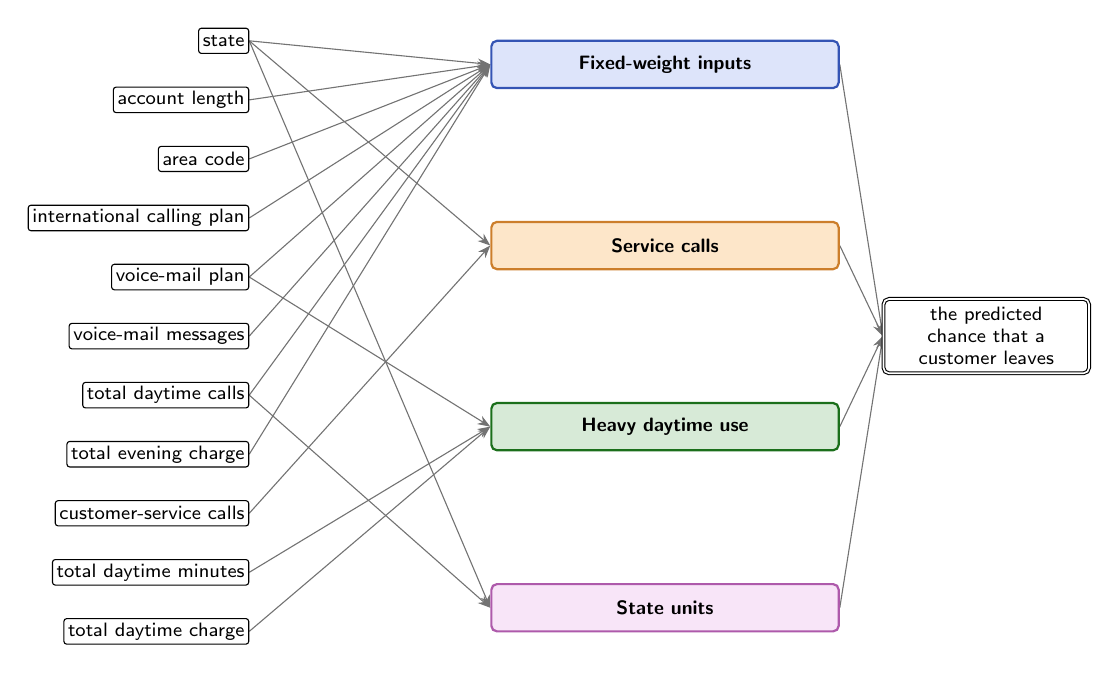
\begin{tikzpicture}[
  font=\sffamily\scriptsize, >={Stealth[length=1.6mm]},
  inp/.style={draw, rounded corners=1pt, fill=white, inner sep=1.5pt, minimum height=3.2mm, anchor=east},
  abox/.style={draw, thick, rounded corners=2pt, align=center, inner sep=3pt, minimum height=6mm, text width=42mm},
  outp/.style={draw, double, rounded corners=2pt, fill=white, align=center, inner sep=3pt, text width=24mm},
  agg/.style={draw=black!55},
]
\node[inp] (i0) at (0,3.75) {state};
\node[inp] (i1) at (0,3.0) {account length};
\node[inp] (i2) at (0,2.25) {area code};
\node[inp] (i3) at (0,1.5) {international calling plan};
\node[inp] (i4) at (0,0.75) {voice-mail plan};
\node[inp] (i5) at (0,-0.0) {voice-mail messages};
\node[inp] (i6) at (0,-0.75) {total daytime calls};
\node[inp] (i7) at (0,-1.5) {total evening charge};
\node[inp] (i8) at (0,-2.25) {customer-service calls};
\node[inp] (i9) at (0,-3.0) {total daytime minutes};
\node[inp] (i10) at (0,-3.75) {total daytime charge};
\node[abox, fill=RoyalBlue!18, draw=RoyalBlue!80!black] (b0) at (5.28,3.45) {\textbf{Fixed-weight inputs}};
\node[abox, fill=BurntOrange!18, draw=BurntOrange!80!black] (b1) at (5.28,1.15) {\textbf{Service calls}};
\node[abox, fill=ForestGreen!18, draw=ForestGreen!80!black] (b2) at (5.28,-1.15) {\textbf{Heavy daytime use}};
\node[abox, fill=Orchid!18, draw=Orchid!80!black] (b3) at (5.28,-3.45) {\textbf{State units}};
\node[outp] (out) at (9.36,0) {the predicted chance that a customer leaves};
\begin{scope}[on background layer]
\draw[->, agg, thin] (i0.east) -- (b0.west);
\draw[->, agg, thin] (i1.east) -- (b0.west);
\draw[->, agg, thin] (i2.east) -- (b0.west);
\draw[->, agg, thin] (i3.east) -- (b0.west);
\draw[->, agg, thin] (i4.east) -- (b0.west);
\draw[->, agg, thin] (i5.east) -- (b0.west);
\draw[->, agg, thin] (i6.east) -- (b0.west);
\draw[->, agg, thin] (i7.east) -- (b0.west);
\draw[->, agg] (b0.east) -- (out.west);
\draw[->, agg, thin] (i0.east) -- (b1.west);
\draw[->, agg, thin] (i8.east) -- (b1.west);
\draw[->, agg] (b1.east) -- (out.west);
\draw[->, agg, thin] (i4.east) -- (b2.west);
\draw[->, agg, thin] (i9.east) -- (b2.west);
\draw[->, agg, thin] (i10.east) -- (b2.west);
\draw[->, agg] (b2.east) -- (out.west);
\draw[->, agg, thin] (i0.east) -- (b3.west);
\draw[->, agg, thin] (i6.east) -- (b3.west);
\draw[->, agg] (b3.east) -- (out.west);
\end{scope}
\end{tikzpicture}}}%
\caption{The whole model: what feeds it, one level down.}
\label{fig:churn100s4c3:parts-ann88}
\end{figure}
\begin{figure}[H]\centering
\resizebox{\ifdim\width>\linewidth\linewidth\else\width\fi}{!}{%
\definecolor{netup}{HTML}{D95F02}\definecolor{netdown}{HTML}{1B9E77}\definecolor{netmixed}{HTML}{7F7F7F}%
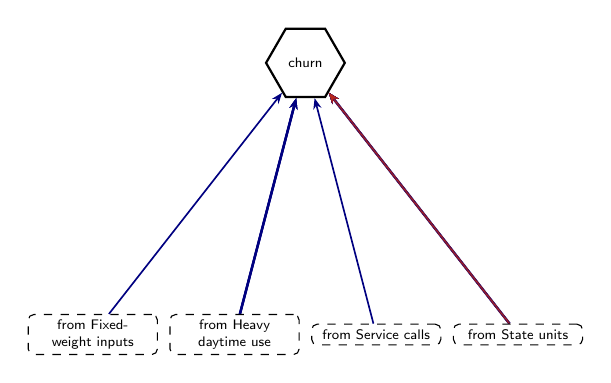
\begin{tikzpicture}[
  font=\sffamily\scriptsize, >={Stealth[length=1.4mm]},
  inp/.style={draw, circle, fill=white, minimum size=3.2mm, inner sep=0pt},
  hid/.style={draw, circle, fill=white, minimum size=5.2mm, inner sep=0.5pt, font=\sffamily\tiny},
  exitbox/.style={draw, thick, rectangle, fill=white, align=center, text width=17mm, minimum height=5mm, inner sep=1.5pt, font=\sffamily\tiny},
  sumbox/.style={draw, thick, dashed, rectangle, fill=white, align=center, text width=17mm, minimum height=5mm, inner sep=1.5pt, font=\sffamily\tiny},
  outp/.style={draw, thick, regular polygon, regular polygon sides=6, fill=white, minimum size=10mm, inner sep=0pt, font=\sffamily\tiny, align=center},
  stub/.style={draw, dashed, rounded corners=2pt, fill=white, align=center, inner sep=2pt, font=\sffamily\tiny, text width=15mm},
  inlab/.style={font=\sffamily\tiny, align=center, text width=15mm, inner sep=1pt, fill=white, fill opacity=0.8, text opacity=1},
  wpos/.style={draw=NavyBlue}, wneg/.style={draw=BrickRed}, wagg/.style={draw=black!45, line width=1.2pt},
  wmix/.style={draw=Plum},
]
\node[outp] (n0) at (3.6,3.45) {churn};
\node[stub] (nfromxxStatexunits) at (6.3,0.0) {from State units};
\node[stub] (nfromxxHeavyxdaytimexuse) at (2.7,0.0) {from Heavy daytime use};
\node[stub] (nfromxxFixedmweightxinputs) at (0.9,0.0) {from Fixed-weight inputs};
\node[stub] (nfromxxServicexcalls) at (4.5,0.0) {from Service calls};
\begin{scope}[on background layer]
\draw[->, wneg, line width=0.64pt] (nfromxxStatexunits) -- (n0);
\draw[->, wneg, line width=0.66pt] (nfromxxStatexunits) -- (n0);
\draw[->, wpos, line width=0.77pt] (nfromxxHeavyxdaytimexuse) -- (n0);
\draw[->, wpos, line width=0.77pt] (nfromxxHeavyxdaytimexuse) -- (n0);
\draw[->, wpos, line width=0.94pt] (nfromxxStatexunits) -- (n0);
\draw[->, wneg, line width=0.44pt] (nfromxxStatexunits) -- (n0);
\draw[->, wneg, line width=0.69pt] (nfromxxStatexunits) -- (n0);
\draw[->, wpos, line width=0.27pt] (nfromxxStatexunits) -- (n0);
\draw[->, wpos, line width=0.91pt] (nfromxxHeavyxdaytimexuse) -- (n0);
\draw[->, wpos, line width=0.27pt] (nfromxxStatexunits) -- (n0);
\draw[->, wneg, line width=0.26pt] (nfromxxStatexunits) -- (n0);
\draw[->, wneg, line width=0.26pt] (nfromxxStatexunits) -- (n0);
\draw[->, wpos, line width=0.27pt] (nfromxxStatexunits) -- (n0);
\draw[->, wpos, line width=0.26pt] (nfromxxStatexunits) -- (n0);
\draw[->, wpos, line width=0.27pt] (nfromxxStatexunits) -- (n0);
\draw[->, wneg, line width=0.30pt] (nfromxxStatexunits) -- (n0);
\draw[->, wpos, line width=0.60pt] (nfromxxFixedmweightxinputs) -- (n0);
\draw[->, wpos, line width=0.60pt] (nfromxxServicexcalls) -- (n0);
\end{scope}
\end{tikzpicture}}%
\caption{The whole model: its units and every connection into them. Blue: positive weight (raises the score); red: negative weight (lowers it); thicker: larger weight. Orange outline and up arrow: raises the final prediction; teal and down arrow: lowers it; grey and double arrow: depends.}
\label{fig:churn100s4c3:units-ann88}
\end{figure}
\paragraph{Hypothesis.} The model adds up four parts into one score: fixed-weight inputs, service calls, heavy daytime use and state units.\,{\scriptsize\textcolor{NavyBlue}{[C054]}}
\paragraph{Evidence.} It is made up of these four parts (each explained below); the score is their sum, which was checked on all 4000 training customers.\,{\scriptsize\textcolor{NavyBlue}{[C054]}} Changing one input at a time across the whole model, an international plan takes a typical customer's chance of leaving from about 1\% to about 18\%, and a voice-mail plan lowers it to below 1\%.\,{\scriptsize\textcolor{NavyBlue}{[C001, C008]}} More voice-mail messages raise it steadily, from about 1\% at 0 to about 6\% at 32 messages, flattening out near the bottom because the predicted chance cannot go much lower.\,{\scriptsize\textcolor{NavyBlue}{[C002]}} More daytime minutes raise it in an uneven way, from about 1\% at 112 minutes to about 6\% at 249 minutes, flattening out near the bottom because the predicted chance cannot go much lower.\,{\scriptsize\textcolor{NavyBlue}{[C003]}} The model ignores evening calls, evening minutes, international calls, the international charge, international minutes, night-time calls, the night-time charge and night-time minutes.\,{\scriptsize\textcolor{NavyBlue}{[C046, C047, C048, C049, C050, C051, C052, C053]}}
\par\noindent{\small Evidence plots: Figure~\ref{fig:churn100s4c3:plot-ann88-0}, Figure~\ref{fig:churn100s4c3:plot-ann88-1}.\par}
\begin{figure}[H]\centering
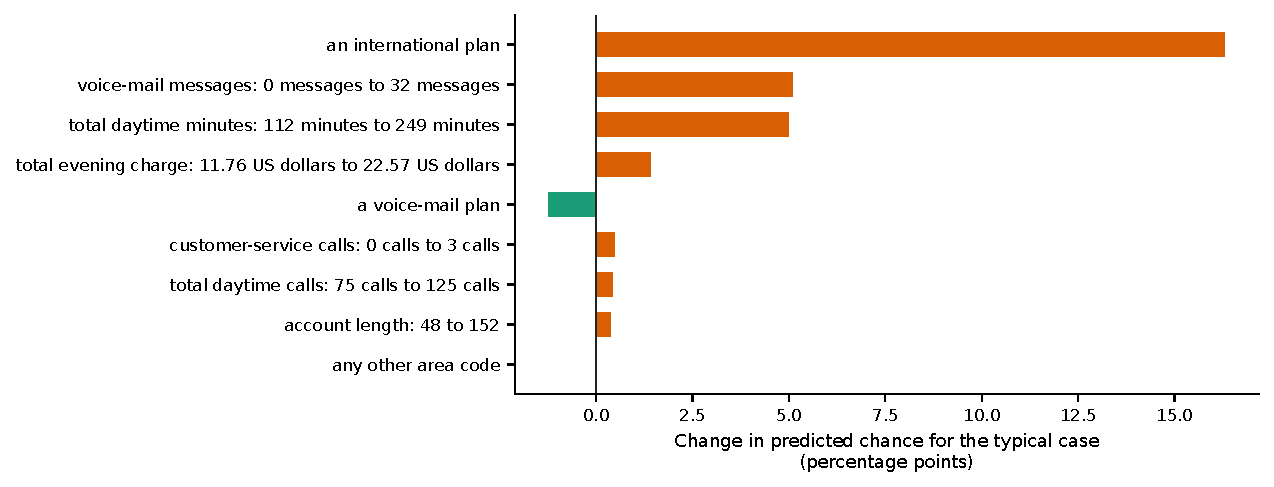
\includegraphics[width=\linewidth,height=0.88\textheight,keepaspectratio]{figures/churn100-s4-c3/ann_88-effects.pdf}
\caption{The whole model: Each input's change in the predicted value for the typical case across the whole model, largest first (orange: raises it, teal: lowers it).}
\label{fig:churn100s4c3:plot-ann88-0}
\end{figure}
\begin{figure}[H]\centering
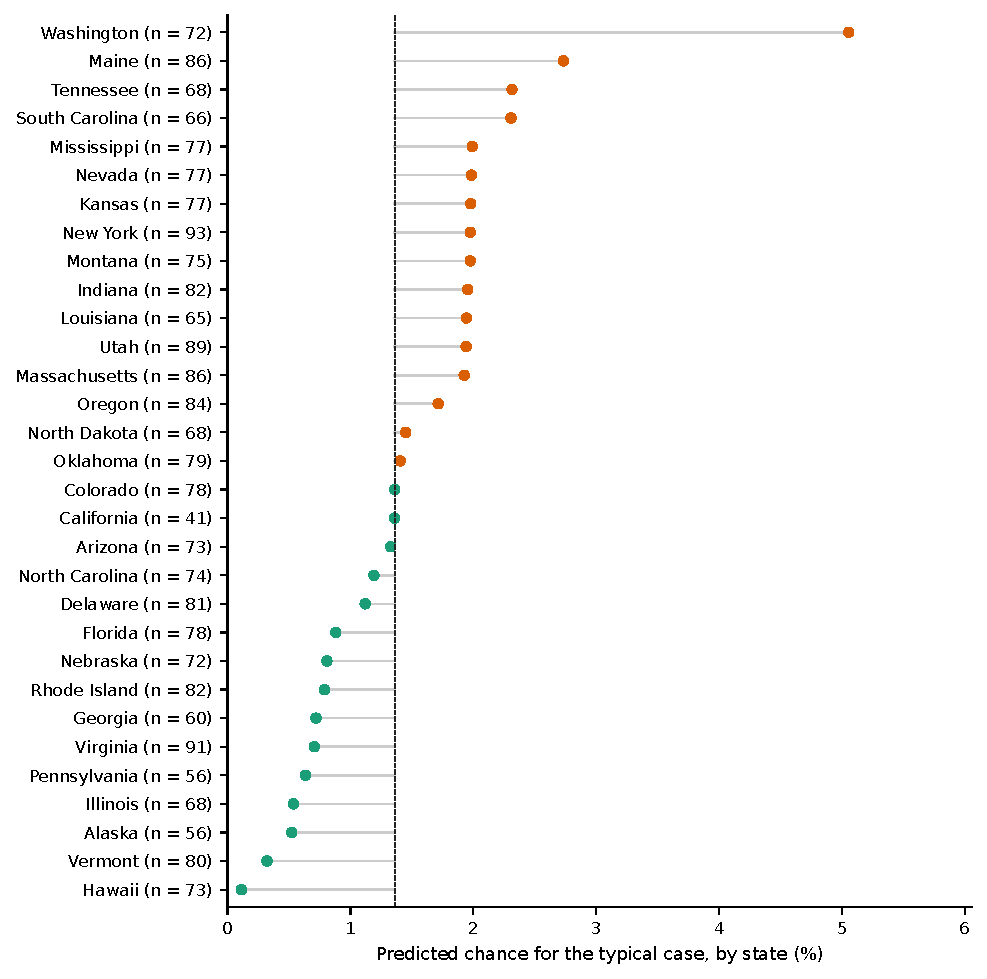
\includegraphics[width=\linewidth,height=0.88\textheight,keepaspectratio]{figures/churn100-s4-c3/ann_88-levels-state.pdf}
\caption{The whole model: Every level of state the model reads: the predicted value for the typical case at that level (dashed: the reference level); n = training customers; grey: few customers or not supported.}
\label{fig:churn100s4c3:plot-ann88-1}
\end{figure}
\par\smallskip\noindent{\small \textbf{Dive deeper:} Fixed-weight inputs (\ref{rd:ann82}); Service calls (\ref{rd:ann87}); Heavy daytime use (\ref{rd:ann85}); State units (\ref{rd:ann86}). Technical detail: \ref{tech:ann88}.\par}
\subsubsection{Fixed-weight inputs}\label{rd:ann82}
\noindent{\footnotesize Part of: The whole model (\ref{rd:ann88}).\par}
\noindent{\small Figure~\ref{fig:churn100s4c3:parts-ann82} shows what feeds this part; Figure~\ref{fig:churn100s4c3:units-ann82} its units and every connection into them (dashed boxes: connections from or to other parts, drawn in their own sections).\par}
\begin{figure}[H]\centering
\resizebox{!}{\ifdim\height>0.5\textheight 0.5\textheight\else\height\fi}{%
\resizebox{\ifdim\width>\linewidth\linewidth\else\width\fi}{!}{%
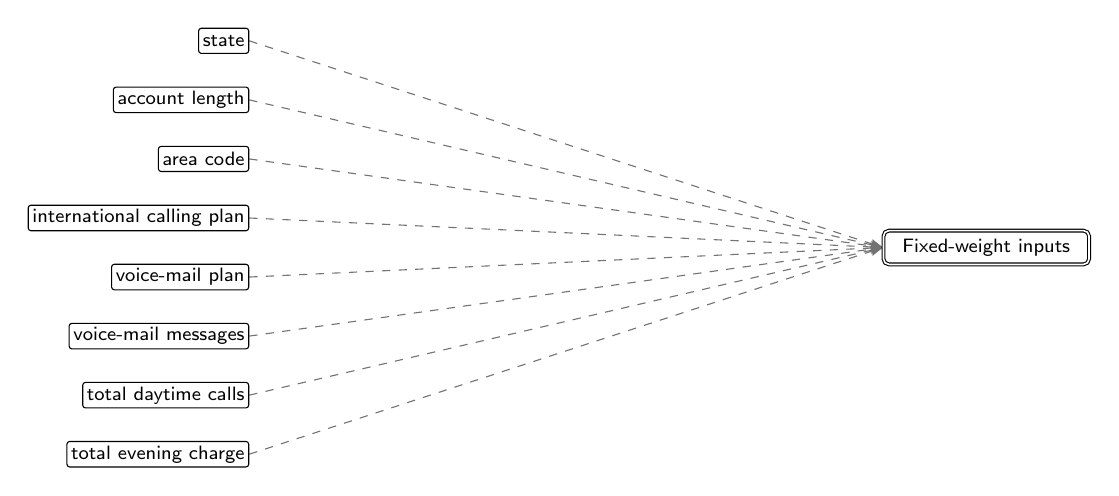
\begin{tikzpicture}[
  font=\sffamily\scriptsize, >={Stealth[length=1.6mm]},
  inp/.style={draw, rounded corners=1pt, fill=white, inner sep=1.5pt, minimum height=3.2mm, anchor=east},
  abox/.style={draw, thick, rounded corners=2pt, align=center, inner sep=3pt, minimum height=6mm, text width=42mm},
  outp/.style={draw, double, rounded corners=2pt, fill=white, align=center, inner sep=3pt, text width=24mm},
  agg/.style={draw=black!55},
]
\node[inp] (i0) at (0,2.625) {state};
\node[inp] (i1) at (0,1.875) {account length};
\node[inp] (i2) at (0,1.125) {area code};
\node[inp] (i3) at (0,0.375) {international calling plan};
\node[inp] (i4) at (0,-0.375) {voice-mail plan};
\node[inp] (i5) at (0,-1.125) {voice-mail messages};
\node[inp] (i6) at (0,-1.875) {total daytime calls};
\node[inp] (i7) at (0,-2.625) {total evening charge};
\node[outp] (out) at (9.36,0) {Fixed-weight inputs};
\begin{scope}[on background layer]
\draw[->, agg, thin, dashed] (i0.east) -- (out.west);
\draw[->, agg, thin, dashed] (i1.east) -- (out.west);
\draw[->, agg, thin, dashed] (i2.east) -- (out.west);
\draw[->, agg, thin, dashed] (i3.east) -- (out.west);
\draw[->, agg, thin, dashed] (i4.east) -- (out.west);
\draw[->, agg, thin, dashed] (i5.east) -- (out.west);
\draw[->, agg, thin, dashed] (i6.east) -- (out.west);
\draw[->, agg, thin, dashed] (i7.east) -- (out.west);
\end{scope}
\end{tikzpicture}}}%
\caption{Fixed-weight inputs: what feeds it, one level down.}
\label{fig:churn100s4c3:parts-ann82}
\end{figure}
\begin{figure}[H]\centering
\resizebox{\ifdim\width>\linewidth\linewidth\else\width\fi}{!}{%
\definecolor{netup}{HTML}{D95F02}\definecolor{netdown}{HTML}{1B9E77}\definecolor{netmixed}{HTML}{7F7F7F}%
\begin{tikzpicture}[
  font=\sffamily\scriptsize, >={Stealth[length=1.4mm]},
  inp/.style={draw, circle, fill=white, minimum size=3.2mm, inner sep=0pt},
  hid/.style={draw, circle, fill=white, minimum size=5.2mm, inner sep=0.5pt, font=\sffamily\tiny},
  exitbox/.style={draw, thick, rectangle, fill=white, align=center, text width=17mm, minimum height=5mm, inner sep=1.5pt, font=\sffamily\tiny},
  sumbox/.style={draw, thick, dashed, rectangle, fill=white, align=center, text width=17mm, minimum height=5mm, inner sep=1.5pt, font=\sffamily\tiny},
  outp/.style={draw, thick, regular polygon, regular polygon sides=6, fill=white, minimum size=10mm, inner sep=0pt, font=\sffamily\tiny, align=center},
  stub/.style={draw, dashed, rounded corners=2pt, fill=white, align=center, inner sep=2pt, font=\sffamily\tiny, text width=15mm},
  inlab/.style={font=\sffamily\tiny, align=center, text width=15mm, inner sep=1pt, fill=white, fill opacity=0.8, text opacity=1},
  wpos/.style={draw=NavyBlue}, wneg/.style={draw=BrickRed}, wagg/.style={draw=black!45, line width=1.2pt},
  wmix/.style={draw=Plum},
]
\node[exitbox] (nidentityxlin) at (5.85,1.9) {Fixed-weight inputs $\uparrow$};
\node[inp, draw=netmixed, very thick] (ngrpxxstate) at (4.5,0.0) {};
\path (ngrpxxstate.south) node[inlab, anchor=north] (labngrpxxstate) {state (31 of 51 used) $\updownarrow$};
\node[inp, draw=netup, very thick] (ninxxaccountxlength) at (1.8,-1.05) {};
\path (ninxxaccountxlength.south) node[inlab, anchor=north] (labninxxaccountxlength) {account length $\uparrow$};
\node[inp, draw=netup, very thick] (ninxxareaxcodex415) at (3.6,-1.05) {};
\path (ninxxareaxcodex415.south) node[inlab, anchor=north] (labninxxareaxcodex415) {area code 415 $\uparrow$};
\node[inp, draw=netup, very thick] (ninxxinternationalxplan) at (2.7,0.0) {};
\path (ninxxinternationalxplan.south) node[inlab, anchor=north] (labninxxinternationalxplan) {an international plan $\uparrow$};
\node[inp, draw=netup, very thick] (ninxxnumberxvmailxmessages) at (9.9,0.0) {};
\path (ninxxnumberxvmailxmessages.south) node[inlab, anchor=north] (labninxxnumberxvmailxmessages) {voice-mail messages $\uparrow$};
\node[inp, draw=netup, very thick] (ninxxtotalxevexcharge) at (8.1,0.0) {};
\path (ninxxtotalxevexcharge.south) node[inlab, anchor=north] (labninxxtotalxevexcharge) {total evening charge $\uparrow$};
\node[inp, draw=netup, very thick] (ninxxtotalxdayxcalls) at (6.3,0.0) {};
\path (ninxxtotalxdayxcalls.south) node[inlab, anchor=north] (labninxxtotalxdayxcalls) {total daytime calls $\uparrow$};
\node[inp, draw=netdown, very thick] (ninxxvoicexmailxplan) at (0.9,0.0) {};
\path (ninxxvoicexmailxplan.south) node[inlab, anchor=north] (labninxxvoicexmailxplan) {a voice-mail plan $\downarrow$};
\node[stub] (ntoxxthexmodelxoutput) at (5.4,3.45) {to the model output};
\begin{scope}[on background layer]
\node[fit=(nidentityxlin) , inner sep=8pt, rounded corners=5pt, fill=BurntOrange!10, draw=BurntOrange!45] (clu0) {};
\draw[->, wpos, line width=0.29pt] (ninxxaccountxlength) -- (nidentityxlin);
\draw[->, wpos, line width=0.25pt] (ninxxareaxcodex415) -- (nidentityxlin);
\draw[->, wpos, line width=0.53pt] (ninxxinternationalxplan) -- (nidentityxlin);
\draw[->, wpos, line width=0.49pt] (ninxxnumberxvmailxmessages) -- (nidentityxlin);
\draw[->, wpos, line width=0.39pt] (ninxxtotalxevexcharge) -- (nidentityxlin);
\draw[->, wpos, line width=0.29pt] (ninxxtotalxdayxcalls) -- (nidentityxlin);
\draw[->, wneg, line width=0.62pt] (ninxxvoicexmailxplan) -- (nidentityxlin);
\draw[->, wpos, line width=0.60pt] (nidentityxlin) -- (ntoxxthexmodelxoutput);
\draw[->, wmix, line width=0.39pt] (ngrpxxstate) -- node[pos=0.8, sloped, above, font=\sffamily\tiny, inner sep=1pt, fill=white, fill opacity=0.8, text opacity=1] {21 edges, -0.40 to +0.18} (nidentityxlin);
\end{scope}
\node[font=\sffamily\scriptsize\bfseries, text=BurntOrange!55!black, anchor=south west, inner sep=1pt, fill=white, fill opacity=0.85, text opacity=1] at (clu0.north west) {Fixed-weight inputs};
\end{tikzpicture}}%
\caption{Fixed-weight inputs: its units and every connection into them. Blue: positive weight (raises the score); red: negative weight (lowers it); thicker: larger weight. Orange outline and up arrow: raises the final prediction; teal and down arrow: lowers it; grey and double arrow: depends.}
\label{fig:churn100s4c3:units-ann82}
\end{figure}
\paragraph{Hypothesis.} This part adds up most inputs with fixed weights: an international plan, voice-mail messages and the evening charge raise the chance of leaving, steadily for the numbers, and a voice-mail plan lowers it.\,{\scriptsize\textcolor{NavyBlue}{[C055, C056, C059, C063]}}
\paragraph{Evidence.} Through it, an international plan takes a typical customer from about 1\% to about 18\%, and a voice-mail plan lowers the chance to below 1\%.\,{\scriptsize\textcolor{NavyBlue}{[C055, C063]}} More voice-mail messages raise it steadily, from about 1\% at 0 to about 6\% at 32 messages, flattening out near the bottom because the predicted chance cannot go much lower.\,{\scriptsize\textcolor{NavyBlue}{[C056]}} A higher evening charge also raises it steadily, from about 1\% at 11.76 US dollars to about 2\% at 22.57 US dollars, flattening out near the bottom because the predicted chance cannot go much lower.\,{\scriptsize\textcolor{NavyBlue}{[C059]}} Through it, the state moves the chance from about 1\% in West Virginia to about 5\% in Washington and about 4\% in Nevada, and to below 1\% in Rhode Island, Hawaii and Vermont (72 to 82 training customers per state).\,{\scriptsize\textcolor{NavyBlue}{[C057, C058, C061, C062, C064]}} Its formula reproduces the part exactly on all 4000 training customers.\,{\scriptsize\textcolor{NavyBlue}{[C083]}}
\par\noindent{\small Evidence plots: Figure~\ref{fig:churn100s4c3:plot-ann82-0}, Figure~\ref{fig:churn100s4c3:plot-ann82-1}, Figure~\ref{fig:churn100s4c3:plot-ann82-2}, Figure~\ref{fig:churn100s4c3:plot-ann82-3}.\par}
\begin{figure}[H]\centering
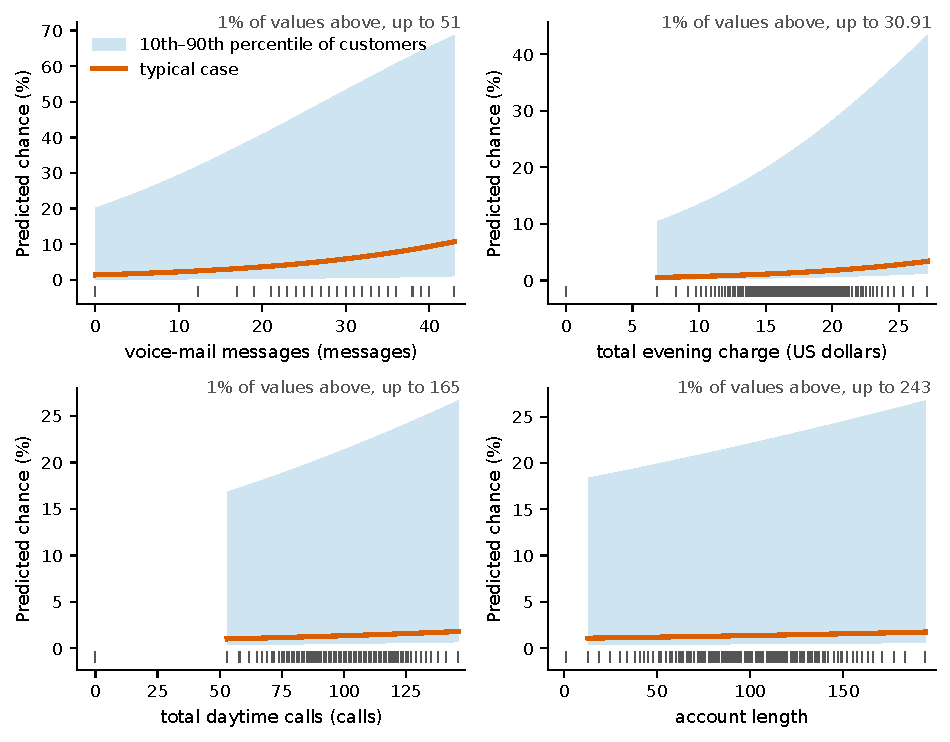
\includegraphics[width=\linewidth,height=0.88\textheight,keepaspectratio]{figures/churn100-s4-c3/ann_82-response.pdf}
\caption{Fixed-weight inputs: Response curves through this part: the typical case (bold), the 10th to 90th percentile of individual customers (band), the fold or step point (dashed) with its spread across them (grey), and the observed values (ticks).}
\label{fig:churn100s4c3:plot-ann82-0}
\end{figure}
\begin{figure}[H]\centering
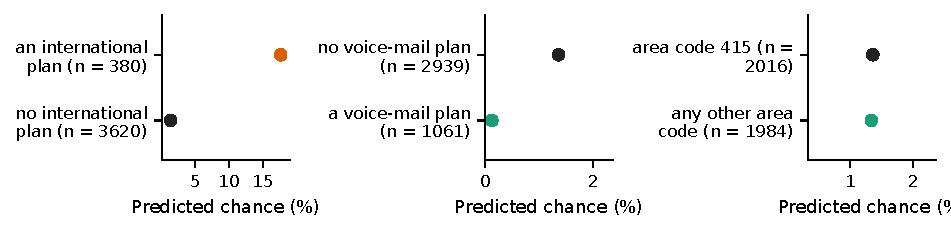
\includegraphics[width=\linewidth,height=0.88\textheight,keepaspectratio]{figures/churn100-s4-c3/ann_82-categories-small.pdf}
\caption{Fixed-weight inputs: The predicted value for the typical case at each level, through this part (n = training customers; grey: fewer than 20).}
\label{fig:churn100s4c3:plot-ann82-1}
\end{figure}
\begin{figure}[H]\centering
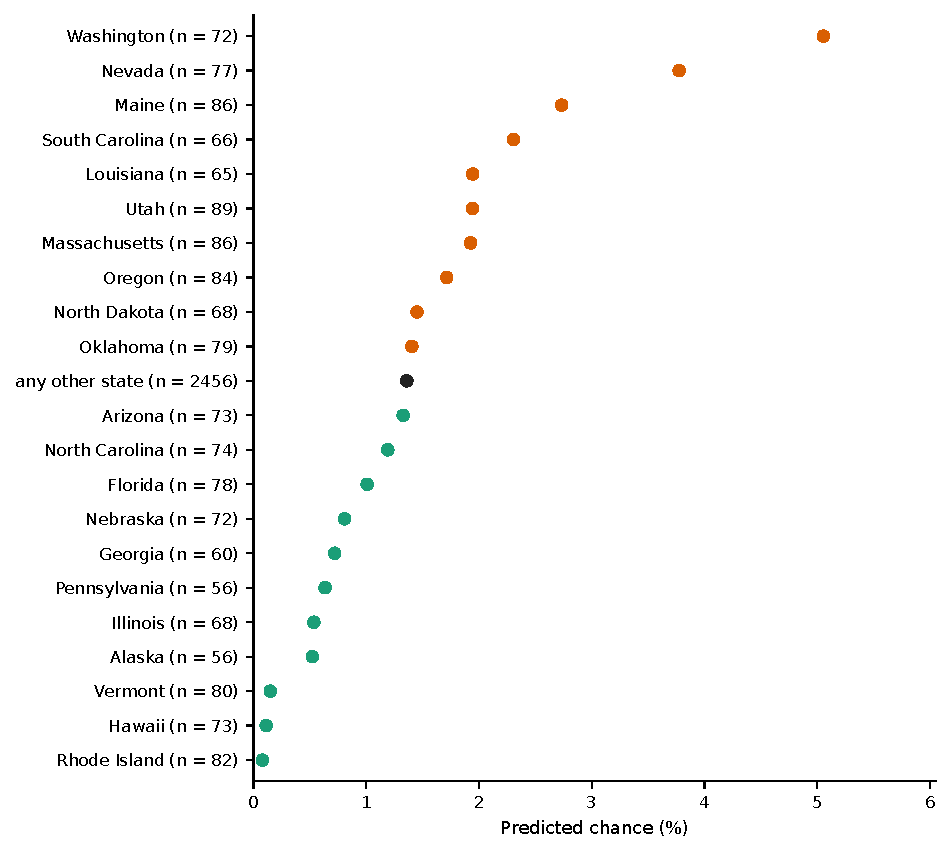
\includegraphics[width=\linewidth,height=0.88\textheight,keepaspectratio]{figures/churn100-s4-c3/ann_82-categories-C057.pdf}
\caption{Fixed-weight inputs: The predicted value for the typical case at each level, through this part (n = training customers; grey: fewer than 20).}
\label{fig:churn100s4c3:plot-ann82-2}
\end{figure}
\begin{figure}[H]\centering
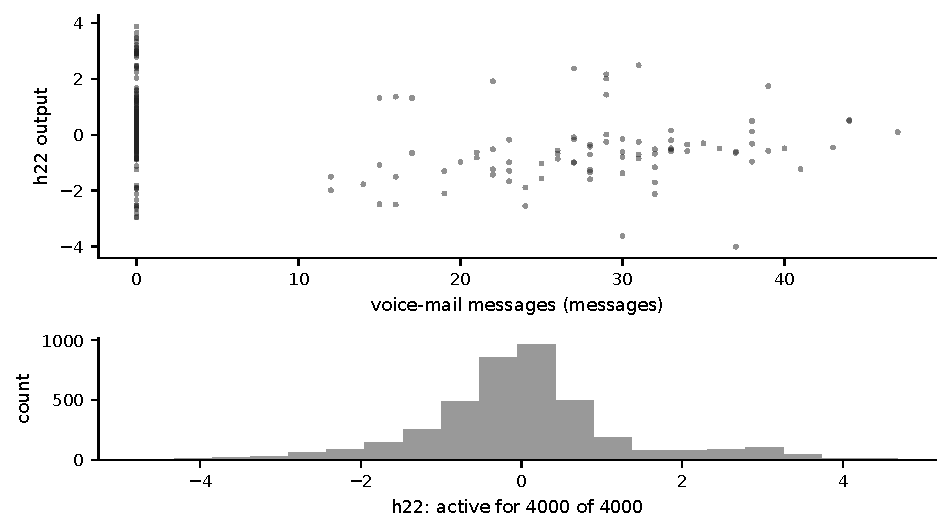
\includegraphics[width=\linewidth,height=0.88\textheight,keepaspectratio]{figures/churn100-s4-c3/ann_82-units.pdf}
\caption{Fixed-weight inputs: This part's hidden units: each unit's output against its main numeric input (top) and how often it is active (bottom).}
\label{fig:churn100s4c3:plot-ann82-3}
\end{figure}
\par\smallskip\noindent{\small Technical detail: \ref{tech:ann82}.\par}
\subsubsection{Service calls}\label{rd:ann87}
\noindent{\footnotesize Part of: The whole model (\ref{rd:ann88}).\par}
\noindent{\small Figure~\ref{fig:churn100s4c3:parts-ann87} shows what feeds this part; Figure~\ref{fig:churn100s4c3:units-ann87} its units and every connection into them (dashed boxes: connections from or to other parts, drawn in their own sections).\par}
\begin{figure}[H]\centering
\resizebox{!}{\ifdim\height>0.5\textheight 0.5\textheight\else\height\fi}{%
\resizebox{\ifdim\width>\linewidth\linewidth\else\width\fi}{!}{%
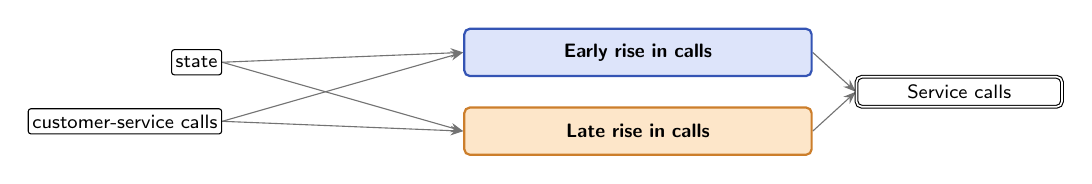
\begin{tikzpicture}[
  font=\sffamily\scriptsize, >={Stealth[length=1.6mm]},
  inp/.style={draw, rounded corners=1pt, fill=white, inner sep=1.5pt, minimum height=3.2mm, anchor=east},
  abox/.style={draw, thick, rounded corners=2pt, align=center, inner sep=3pt, minimum height=6mm, text width=42mm},
  outp/.style={draw, double, rounded corners=2pt, fill=white, align=center, inner sep=3pt, text width=24mm},
  agg/.style={draw=black!55},
]
\node[inp] (i0) at (0,0.375) {state};
\node[inp] (i1) at (0,-0.375) {customer-service calls};
\node[abox, fill=RoyalBlue!18, draw=RoyalBlue!80!black] (b0) at (5.28,0.5) {\textbf{Early rise in calls}};
\node[abox, fill=BurntOrange!18, draw=BurntOrange!80!black] (b1) at (5.28,-0.5) {\textbf{Late rise in calls}};
\node[outp] (out) at (9.36,0) {Service calls};
\begin{scope}[on background layer]
\draw[->, agg, thin] (i0.east) -- (b0.west);
\draw[->, agg, thin] (i1.east) -- (b0.west);
\draw[->, agg] (b0.east) -- (out.west);
\draw[->, agg, thin] (i0.east) -- (b1.west);
\draw[->, agg, thin] (i1.east) -- (b1.west);
\draw[->, agg] (b1.east) -- (out.west);
\end{scope}
\end{tikzpicture}}}%
\caption{Service calls: what feeds it, one level down.}
\label{fig:churn100s4c3:parts-ann87}
\end{figure}
\begin{figure}[H]\centering
\resizebox{\ifdim\width>\linewidth\linewidth\else\width\fi}{!}{%
\definecolor{netup}{HTML}{D95F02}\definecolor{netdown}{HTML}{1B9E77}\definecolor{netmixed}{HTML}{7F7F7F}%
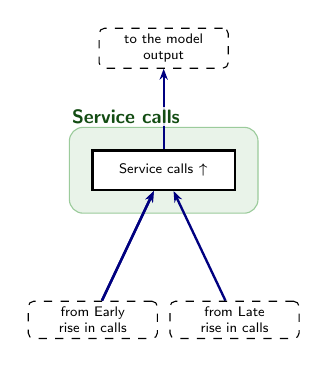
\begin{tikzpicture}[
  font=\sffamily\scriptsize, >={Stealth[length=1.4mm]},
  inp/.style={draw, circle, fill=white, minimum size=3.2mm, inner sep=0pt},
  hid/.style={draw, circle, fill=white, minimum size=5.2mm, inner sep=0.5pt, font=\sffamily\tiny},
  exitbox/.style={draw, thick, rectangle, fill=white, align=center, text width=17mm, minimum height=5mm, inner sep=1.5pt, font=\sffamily\tiny},
  sumbox/.style={draw, thick, dashed, rectangle, fill=white, align=center, text width=17mm, minimum height=5mm, inner sep=1.5pt, font=\sffamily\tiny},
  outp/.style={draw, thick, regular polygon, regular polygon sides=6, fill=white, minimum size=10mm, inner sep=0pt, font=\sffamily\tiny, align=center},
  stub/.style={draw, dashed, rounded corners=2pt, fill=white, align=center, inner sep=2pt, font=\sffamily\tiny, text width=15mm},
  inlab/.style={font=\sffamily\tiny, align=center, text width=15mm, inner sep=1pt, fill=white, fill opacity=0.8, text opacity=1},
  wpos/.style={draw=NavyBlue}, wneg/.style={draw=BrickRed}, wagg/.style={draw=black!45, line width=1.2pt},
  wmix/.style={draw=Plum},
]
\node[exitbox] (nidentityxsvc) at (1.8,1.9) {Service calls $\uparrow$};
\node[stub] (nfromxxLatexrisexinxcalls) at (2.7,0.0) {from Late rise in calls};
\node[stub] (nfromxxEarlyxrisexinxcalls) at (0.9,0.0) {from Early rise in calls};
\node[stub] (ntoxxthexmodelxoutput) at (1.8,3.45) {to the model output};
\begin{scope}[on background layer]
\node[fit=(nidentityxsvc) , inner sep=8pt, rounded corners=5pt, fill=ForestGreen!10, draw=ForestGreen!45] (clu0) {};
\draw[->, wpos, line width=0.85pt] (nfromxxLatexrisexinxcalls) -- (nidentityxsvc);
\draw[->, wpos, line width=0.91pt] (nfromxxEarlyxrisexinxcalls) -- (nidentityxsvc);
\draw[->, wpos, line width=0.86pt] (nfromxxEarlyxrisexinxcalls) -- (nidentityxsvc);
\draw[->, wpos, line width=0.60pt] (nidentityxsvc) -- (ntoxxthexmodelxoutput);
\end{scope}
\node[font=\sffamily\scriptsize\bfseries, text=ForestGreen!55!black, anchor=south west, inner sep=1pt, fill=white, fill opacity=0.85, text opacity=1] at (clu0.north west) {Service calls};
\end{tikzpicture}}%
\caption{Service calls: its units and every connection into them. Blue: positive weight (raises the score); red: negative weight (lowers it); thicker: larger weight. Orange outline and up arrow: raises the final prediction; teal and down arrow: lowers it; grey and double arrow: depends.}
\label{fig:churn100s4c3:units-ann87}
\end{figure}
\paragraph{Hypothesis.} This part raises the chance of leaving with calls to customer service, slowly at first, then faster from about 3 calls upwards; it adds up two parts.\,{\scriptsize\textcolor{NavyBlue}{[C090, C089]}}
\paragraph{Evidence.} It is made of two parts that are added: an early rise and a late rise in calls to customer service.\,{\scriptsize\textcolor{NavyBlue}{[C090]}} From about 3 calls upwards it adds to the chance slowly at first, then faster: for a typical such customer, 4 calls take it from about 1\% to about 10\%, flattening out near the bottom because the predicted chance cannot go much lower.\,{\scriptsize\textcolor{NavyBlue}{[C089]}} Up to 3 calls the chance rises slowly at first, then faster, from about 1\% to about 2\% for a typical customer, flattening out near the bottom because the predicted chance cannot go much lower.\,{\scriptsize\textcolor{NavyBlue}{[C084]}} That early rise happens only outside Nebraska, California and Colorado: in Nebraska the chance stays at about 1\% from 0 to 3 calls, against a rise from about 1\% to about 2\% elsewhere, slowly at first, then faster, flattening out near the bottom because the predicted chance cannot go much lower.\,{\scriptsize\textcolor{NavyBlue}{[C088]}}
\par\noindent{\small Evidence plots: Figure~\ref{fig:churn100s4c3:plot-ann87-0}, Figure~\ref{fig:churn100s4c3:plot-ann87-1}, Figure~\ref{fig:churn100s4c3:plot-ann87-2}, Figure~\ref{fig:churn100s4c3:plot-ann87-3}, Figure~\ref{fig:churn100s4c3:plot-ann87-4}.\par}
\par\noindent{\small Figure~\ref{fig:churn100s4c3:plot-ann87-3} shows this part's own output, unit h23: it switches on at about 2.827 calls of customer-service calls, and is zero below.\par}
\begin{figure}[H]\centering
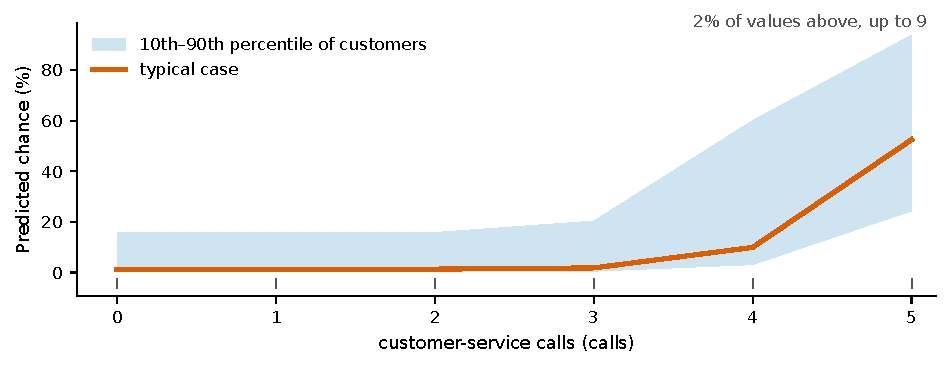
\includegraphics[width=\linewidth,height=0.88\textheight,keepaspectratio]{figures/churn100-s4-c3/ann_87-response.pdf}
\caption{Service calls: Response curves through this part: the typical case (bold), the 10th to 90th percentile of individual customers (band), the fold or step point (dashed) with its spread across them (grey), and the observed values (ticks).}
\label{fig:churn100s4c3:plot-ann87-0}
\end{figure}
\begin{figure}[H]\centering
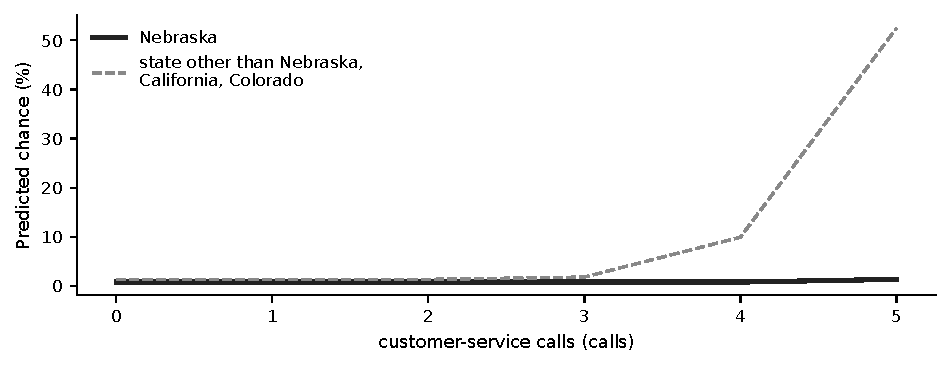
\includegraphics[width=\linewidth,height=0.88\textheight,keepaspectratio]{figures/churn100-s4-c3/ann_87-interaction.pdf}
\caption{Service calls: How the effect differs between groups: one curve per group, for the typical case of each group.}
\label{fig:churn100s4c3:plot-ann87-1}
\end{figure}
\begin{figure}[H]\centering
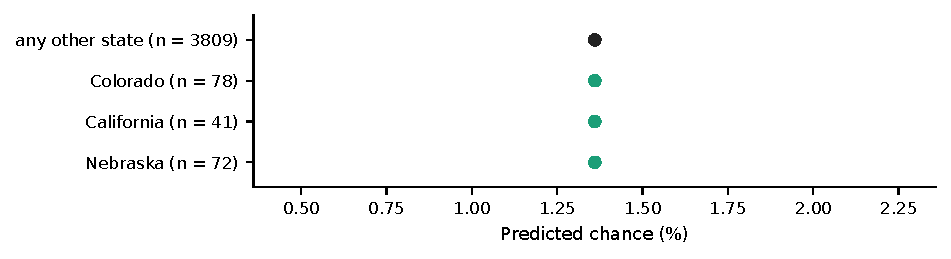
\includegraphics[width=\linewidth,height=0.88\textheight,keepaspectratio]{figures/churn100-s4-c3/ann_87-categories-small.pdf}
\caption{Service calls: The predicted value for the typical case at each level, through this part (n = training customers; grey: fewer than 20).}
\label{fig:churn100s4c3:plot-ann87-2}
\end{figure}
\begin{figure}[H]\centering
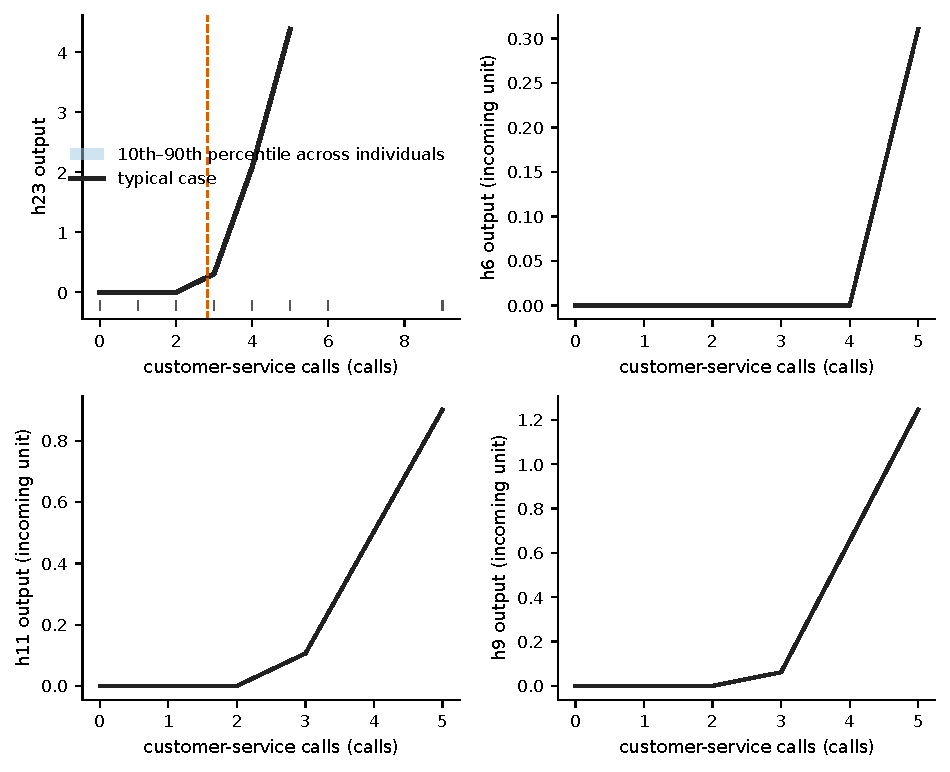
\includegraphics[width=\linewidth,height=0.88\textheight,keepaspectratio]{figures/churn100-s4-c3/ann_87-partial-identity_svc.pdf}
\caption{Service calls: This part's own output, unit h23 (combines 3 non-linear units), on its own scale (its activation), with every other input at the typical case; it is active for 831 of 4000. Bold: the typical case; band: 10th to 90th percentile across individuals; dashed: where it switches on; ticks: the data.}
\label{fig:churn100s4c3:plot-ann87-3}
\end{figure}
\begin{figure}[H]\centering
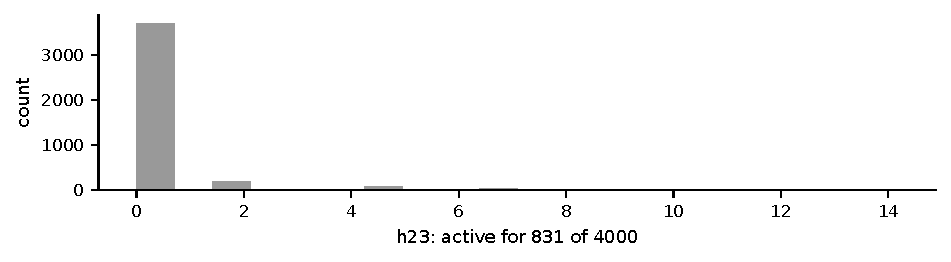
\includegraphics[width=\linewidth,height=0.88\textheight,keepaspectratio]{figures/churn100-s4-c3/ann_87-units.pdf}
\caption{Service calls: This part's hidden units: each unit's output against its main numeric input (top) and how often it is active (bottom).}
\label{fig:churn100s4c3:plot-ann87-4}
\end{figure}
\par\smallskip\noindent{\small \textbf{Dive deeper:} Early rise in calls (\ref{rd:ann84}); Late rise in calls (\ref{rd:ann83}). Technical detail: \ref{tech:ann87}.\par}
\subsubsection{Early rise in calls}\label{rd:ann84}
\noindent{\footnotesize Part of: Service calls (\ref{rd:ann87}).\par}
\noindent{\small Figure~\ref{fig:churn100s4c3:parts-ann84} shows what feeds this part; Figure~\ref{fig:churn100s4c3:units-ann84} its units and every connection into them (dashed boxes: connections from or to other parts, drawn in their own sections).\par}
\begin{figure}[H]\centering
\resizebox{!}{\ifdim\height>0.5\textheight 0.5\textheight\else\height\fi}{%
\resizebox{\ifdim\width>\linewidth\linewidth\else\width\fi}{!}{%
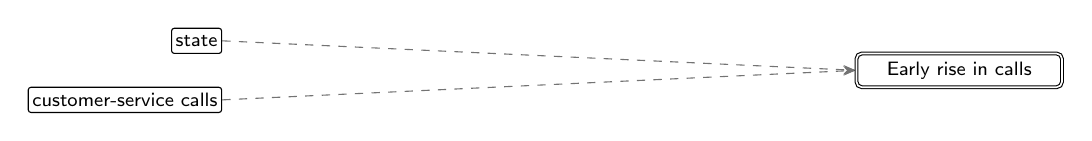
\begin{tikzpicture}[
  font=\sffamily\scriptsize, >={Stealth[length=1.6mm]},
  inp/.style={draw, rounded corners=1pt, fill=white, inner sep=1.5pt, minimum height=3.2mm, anchor=east},
  abox/.style={draw, thick, rounded corners=2pt, align=center, inner sep=3pt, minimum height=6mm, text width=42mm},
  outp/.style={draw, double, rounded corners=2pt, fill=white, align=center, inner sep=3pt, text width=24mm},
  agg/.style={draw=black!55},
]
\node[inp] (i0) at (0,0.375) {state};
\node[inp] (i1) at (0,-0.375) {customer-service calls};
\node[outp] (out) at (9.36,0) {Early rise in calls};
\begin{scope}[on background layer]
\draw[->, agg, thin, dashed] (i0.east) -- (out.west);
\draw[->, agg, thin, dashed] (i1.east) -- (out.west);
\end{scope}
\end{tikzpicture}}}%
\caption{Early rise in calls: what feeds it, one level down.}
\label{fig:churn100s4c3:parts-ann84}
\end{figure}
\begin{figure}[H]\centering
\resizebox{\ifdim\width>\linewidth\linewidth\else\width\fi}{!}{%
\definecolor{netup}{HTML}{D95F02}\definecolor{netdown}{HTML}{1B9E77}\definecolor{netmixed}{HTML}{7F7F7F}%
\begin{tikzpicture}[
  font=\sffamily\scriptsize, >={Stealth[length=1.4mm]},
  inp/.style={draw, circle, fill=white, minimum size=3.2mm, inner sep=0pt},
  hid/.style={draw, circle, fill=white, minimum size=5.2mm, inner sep=0.5pt, font=\sffamily\tiny},
  exitbox/.style={draw, thick, rectangle, fill=white, align=center, text width=17mm, minimum height=5mm, inner sep=1.5pt, font=\sffamily\tiny},
  sumbox/.style={draw, thick, dashed, rectangle, fill=white, align=center, text width=17mm, minimum height=5mm, inner sep=1.5pt, font=\sffamily\tiny},
  outp/.style={draw, thick, regular polygon, regular polygon sides=6, fill=white, minimum size=10mm, inner sep=0pt, font=\sffamily\tiny, align=center},
  stub/.style={draw, dashed, rounded corners=2pt, fill=white, align=center, inner sep=2pt, font=\sffamily\tiny, text width=15mm},
  inlab/.style={font=\sffamily\tiny, align=center, text width=15mm, inner sep=1pt, fill=white, fill opacity=0.8, text opacity=1},
  wpos/.style={draw=NavyBlue}, wneg/.style={draw=BrickRed}, wagg/.style={draw=black!45, line width=1.2pt},
  wmix/.style={draw=Plum},
]
\node[hid] (n6713) at (1.9,3.25) {h9};
\node[hid] (n9436) at (1.9,1.9) {h11};
\node[inp, draw=netup, very thick] (ninxxnumberxcustomerxservicexcalls) at (1.0,0.0) {};
\path (ninxxnumberxcustomerxservicexcalls.south) node[inlab, anchor=north] (labninxxnumberxcustomerxservicexcalls) {customer-service calls $\uparrow$};
\node[inp, draw=netmixed, very thick] (ngrpxxstate) at (2.8,0.0) {};
\path (ngrpxxstate.south) node[inlab, anchor=north] (labngrpxxstate) {state (31 of 51 used) $\updownarrow$};
\node[stub] (ntoxxServicexcalls) at (1.9,4.8) {to Service calls};
\begin{scope}[on background layer]
\node[fit=(n6713) (n9436) , inner sep=8pt, rounded corners=5pt, fill=ForestGreen!10, draw=ForestGreen!45] (clu0) {};
\draw[->, wpos, line width=0.77pt] (n9436) -- (n6713);
\draw[->, wpos, line width=0.43pt] (ninxxnumberxcustomerxservicexcalls) -- (n9436);
\draw[->, wpos, line width=0.91pt] (n9436) -- (ntoxxServicexcalls);
\draw[->, wpos, line width=0.86pt] (n6713) -- (ntoxxServicexcalls);
\draw[->, wneg, line width=0.64pt] (ngrpxxstate) -- node[pos=0.8, sloped, above, font=\sffamily\tiny, inner sep=1pt, fill=white, fill opacity=0.8, text opacity=1] {-1.12} (n9436);
\end{scope}
\node[font=\sffamily\scriptsize\bfseries, text=ForestGreen!55!black, anchor=south west, inner sep=1pt, fill=white, fill opacity=0.85, text opacity=1] at (clu0.north west) {Early rise in calls};
\end{tikzpicture}}%
\caption{Early rise in calls: its units and every connection into them. Blue: positive weight (raises the score); red: negative weight (lowers it); thicker: larger weight. Orange outline and up arrow: raises the final prediction; teal and down arrow: lowers it; grey and double arrow: depends.}
\label{fig:churn100s4c3:units-ann84}
\end{figure}
\paragraph{Hypothesis.} This part raises the chance of leaving from about 3 customer-service calls upwards, in an uneven way.\,{\scriptsize\textcolor{NavyBlue}{[C094]}}
\paragraph{Evidence.} It acts on 830 of 4000 training customers, 213 of whom left; for the typical customer it acts on, the chance is about 1\% without it and about 2\% with it.\,{\scriptsize\textcolor{NavyBlue}{[C095]}} Through it, calls add to the chance only from about 3 calls upwards, in an uneven way: for a typical such customer, 4 calls take it from about 1\% to about 10\%, flattening out near the bottom because the predicted chance cannot go much lower.\,{\scriptsize\textcolor{NavyBlue}{[C094]}} Up to 3 calls it raises the chance slowly at first, then faster, but only outside Nebraska: there from about 1\% to about 2\%, while in Nebraska it stays at about 1\%, flattening out near the bottom because the predicted chance cannot go much lower.\,{\scriptsize\textcolor{NavyBlue}{[C093]}} Its formula reproduces the part exactly on all 4000 training customers.\,{\scriptsize\textcolor{NavyBlue}{[C096]}}
\par\noindent{\small Evidence plots: Figure~\ref{fig:churn100s4c3:plot-ann84-0}, Figure~\ref{fig:churn100s4c3:plot-ann84-1}, Figure~\ref{fig:churn100s4c3:plot-ann84-2}, Figure~\ref{fig:churn100s4c3:plot-ann84-3}, Figure~\ref{fig:churn100s4c3:plot-ann84-4}, Figure~\ref{fig:churn100s4c3:plot-ann84-5}.\par}
\par\noindent{\small Figure~\ref{fig:churn100s4c3:plot-ann84-3} shows this part's own output, unit h11: it switches on at about 2.734 calls of customer-service calls, and is zero below.\par}
\par\noindent{\small Figure~\ref{fig:churn100s4c3:plot-ann84-4} shows this part's own output, unit h9: it switches on at about 2.896 calls of customer-service calls, and is zero below.\par}
\begin{figure}[H]\centering
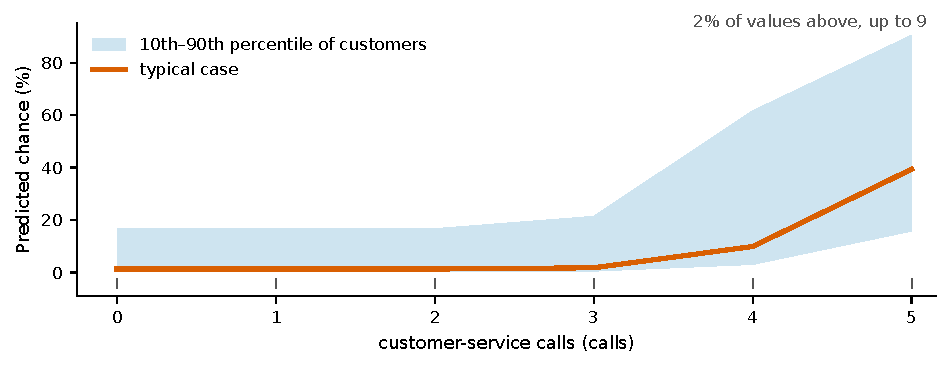
\includegraphics[width=\linewidth,height=0.88\textheight,keepaspectratio]{figures/churn100-s4-c3/ann_84-response.pdf}
\caption{Early rise in calls: Response curves through this part: the typical case (bold), the 10th to 90th percentile of individual customers (band), the fold or step point (dashed) with its spread across them (grey), and the observed values (ticks).}
\label{fig:churn100s4c3:plot-ann84-0}
\end{figure}
\begin{figure}[H]\centering
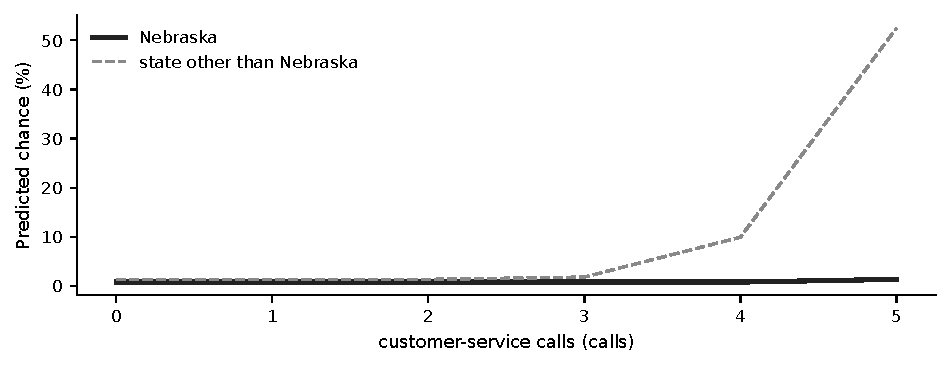
\includegraphics[width=\linewidth,height=0.88\textheight,keepaspectratio]{figures/churn100-s4-c3/ann_84-interaction.pdf}
\caption{Early rise in calls: How the effect differs between groups: one curve per group, for the typical case of each group.}
\label{fig:churn100s4c3:plot-ann84-1}
\end{figure}
\begin{figure}[H]\centering
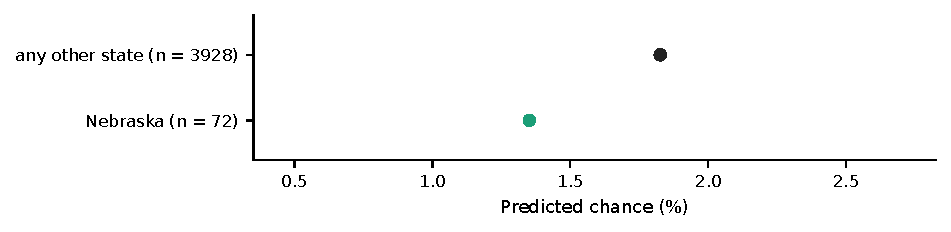
\includegraphics[width=\linewidth,height=0.88\textheight,keepaspectratio]{figures/churn100-s4-c3/ann_84-categories-small.pdf}
\caption{Early rise in calls: The predicted value for the typical case at each level, through this part (n = training customers; grey: fewer than 20).}
\label{fig:churn100s4c3:plot-ann84-2}
\end{figure}
\begin{figure}[H]\centering
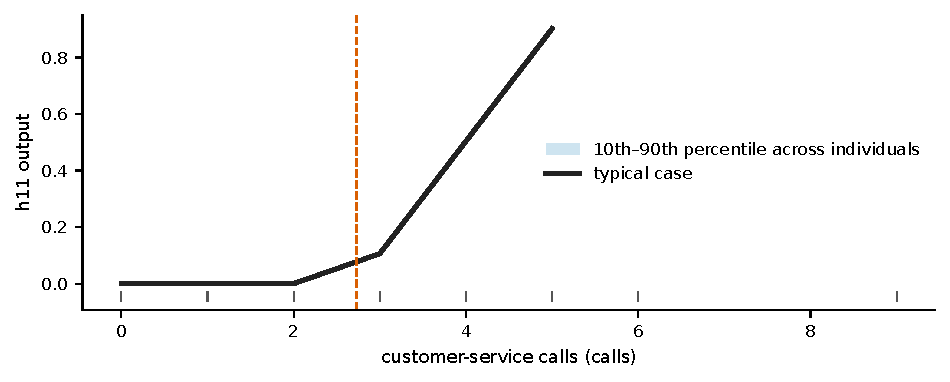
\includegraphics[width=\linewidth,height=0.88\textheight,keepaspectratio]{figures/churn100-s4-c3/ann_84-partial-9436.pdf}
\caption{Early rise in calls: This part's own output, unit h11 (the output of 'Early rise in calls'), on its own scale (its activation), with every other input at the typical case; it is active for 830 of 4000. Bold: the typical case; band: 10th to 90th percentile across individuals; dashed: where it switches on; ticks: the data.}
\label{fig:churn100s4c3:plot-ann84-3}
\end{figure}
\begin{figure}[H]\centering
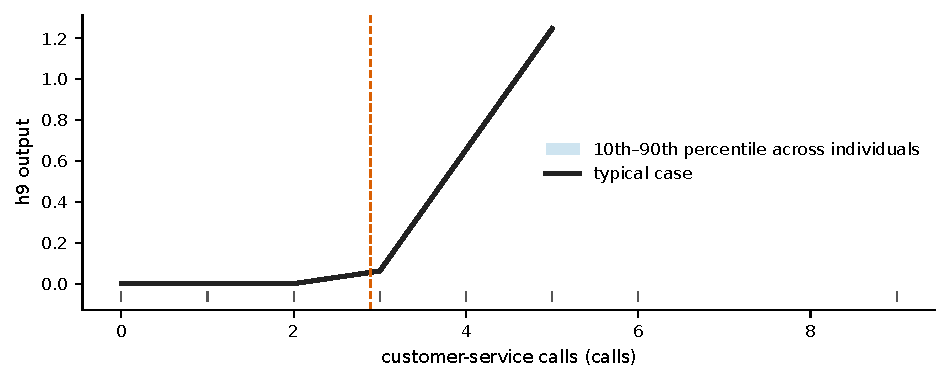
\includegraphics[width=\linewidth,height=0.88\textheight,keepaspectratio]{figures/churn100-s4-c3/ann_84-partial-6713.pdf}
\caption{Early rise in calls: This part's own output, unit h9 (the output of 'Early rise in calls'), on its own scale (its activation), with every other input at the typical case; it is active for 830 of 4000. Bold: the typical case; band: 10th to 90th percentile across individuals; dashed: where it switches on; ticks: the data.}
\label{fig:churn100s4c3:plot-ann84-4}
\end{figure}
\begin{figure}[H]\centering
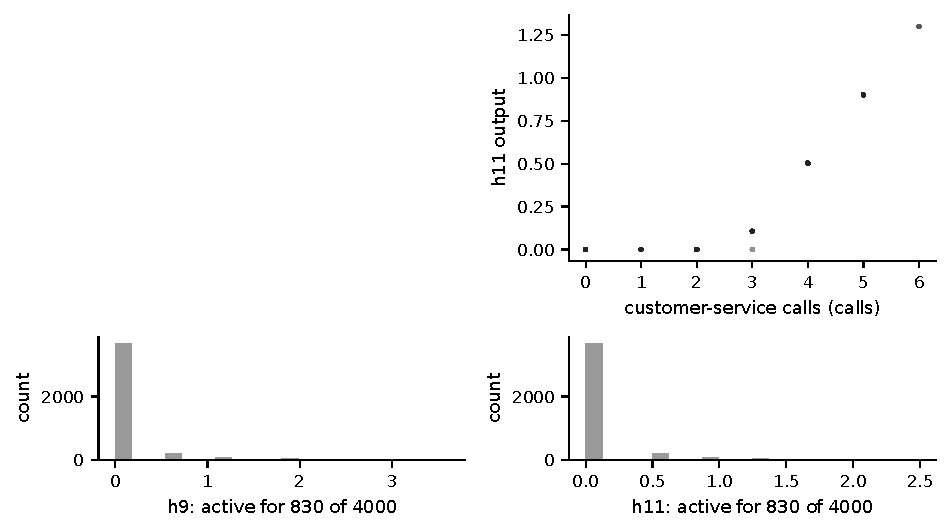
\includegraphics[width=\linewidth,height=0.88\textheight,keepaspectratio]{figures/churn100-s4-c3/ann_84-units.pdf}
\caption{Early rise in calls: This part's hidden units: each unit's output against its main numeric input (top) and how often it is active (bottom).}
\label{fig:churn100s4c3:plot-ann84-5}
\end{figure}
\par\smallskip\noindent{\small Technical detail: \ref{tech:ann84}.\par}
\subsubsection{Late rise in calls}\label{rd:ann83}
\noindent{\footnotesize Part of: Service calls (\ref{rd:ann87}).\par}
\noindent{\small Figure~\ref{fig:churn100s4c3:parts-ann83} shows what feeds this part; Figure~\ref{fig:churn100s4c3:units-ann83} its units and every connection into them (dashed boxes: connections from or to other parts, drawn in their own sections).\par}
\begin{figure}[H]\centering
\resizebox{!}{\ifdim\height>0.5\textheight 0.5\textheight\else\height\fi}{%
\resizebox{\ifdim\width>\linewidth\linewidth\else\width\fi}{!}{%
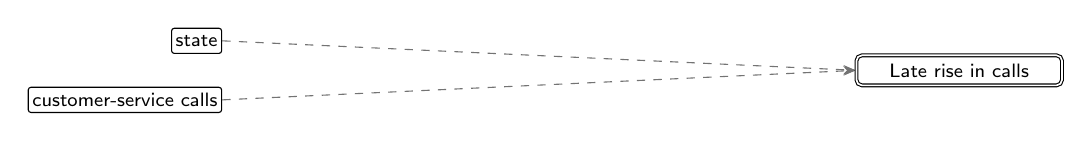
\begin{tikzpicture}[
  font=\sffamily\scriptsize, >={Stealth[length=1.6mm]},
  inp/.style={draw, rounded corners=1pt, fill=white, inner sep=1.5pt, minimum height=3.2mm, anchor=east},
  abox/.style={draw, thick, rounded corners=2pt, align=center, inner sep=3pt, minimum height=6mm, text width=42mm},
  outp/.style={draw, double, rounded corners=2pt, fill=white, align=center, inner sep=3pt, text width=24mm},
  agg/.style={draw=black!55},
]
\node[inp] (i0) at (0,0.375) {state};
\node[inp] (i1) at (0,-0.375) {customer-service calls};
\node[outp] (out) at (9.36,0) {Late rise in calls};
\begin{scope}[on background layer]
\draw[->, agg, thin, dashed] (i0.east) -- (out.west);
\draw[->, agg, thin, dashed] (i1.east) -- (out.west);
\end{scope}
\end{tikzpicture}}}%
\caption{Late rise in calls: what feeds it, one level down.}
\label{fig:churn100s4c3:parts-ann83}
\end{figure}
\begin{figure}[H]\centering
\resizebox{\ifdim\width>\linewidth\linewidth\else\width\fi}{!}{%
\definecolor{netup}{HTML}{D95F02}\definecolor{netdown}{HTML}{1B9E77}\definecolor{netmixed}{HTML}{7F7F7F}%
\begin{tikzpicture}[
  font=\sffamily\scriptsize, >={Stealth[length=1.4mm]},
  inp/.style={draw, circle, fill=white, minimum size=3.2mm, inner sep=0pt},
  hid/.style={draw, circle, fill=white, minimum size=5.2mm, inner sep=0.5pt, font=\sffamily\tiny},
  exitbox/.style={draw, thick, rectangle, fill=white, align=center, text width=17mm, minimum height=5mm, inner sep=1.5pt, font=\sffamily\tiny},
  sumbox/.style={draw, thick, dashed, rectangle, fill=white, align=center, text width=17mm, minimum height=5mm, inner sep=1.5pt, font=\sffamily\tiny},
  outp/.style={draw, thick, regular polygon, regular polygon sides=6, fill=white, minimum size=10mm, inner sep=0pt, font=\sffamily\tiny, align=center},
  stub/.style={draw, dashed, rounded corners=2pt, fill=white, align=center, inner sep=2pt, font=\sffamily\tiny, text width=15mm},
  inlab/.style={font=\sffamily\tiny, align=center, text width=15mm, inner sep=1pt, fill=white, fill opacity=0.8, text opacity=1},
  wpos/.style={draw=NavyBlue}, wneg/.style={draw=BrickRed}, wagg/.style={draw=black!45, line width=1.2pt},
  wmix/.style={draw=Plum},
]
\node[exitbox] (n5268) at (1.8,3.25) {Late rise in calls $\uparrow$};
\node[hid] (n12374) at (1.05,1.9) {h15};
\node[hid] (n349) at (2.55,1.9) {h1};
\node[inp, draw=netmixed, very thick] (ngrpxxstate) at (2.7,0.0) {};
\path (ngrpxxstate.south) node[inlab, anchor=north] (labngrpxxstate) {state (31 of 51 used) $\updownarrow$};
\node[inp, draw=netup, very thick] (ninxxnumberxcustomerxservicexcalls) at (0.9,0.0) {};
\path (ninxxnumberxcustomerxservicexcalls.south) node[inlab, anchor=north] (labninxxnumberxcustomerxservicexcalls) {customer-service calls $\uparrow$};
\node[stub] (ntoxxServicexcalls) at (1.8,4.8) {to Service calls};
\begin{scope}[on background layer]
\node[fit=(n5268) (n12374) (n349) , inner sep=8pt, rounded corners=5pt, fill=ForestGreen!10, draw=ForestGreen!45] (clu0) {};
\draw[->, wneg, line width=0.74pt] (n349) -- (n5268);
\draw[->, wpos, line width=0.34pt] (n12374) -- (n5268);
\draw[->, wpos, line width=0.36pt] (ninxxnumberxcustomerxservicexcalls) -- (n5268);
\draw[->, wpos, line width=0.51pt] (ninxxnumberxcustomerxservicexcalls) -- (n12374);
\draw[->, wpos, line width=0.85pt] (n5268) -- (ntoxxServicexcalls);
\draw[->, wmix, line width=0.90pt] (ngrpxxstate) -- node[pos=0.8, sloped, above, font=\sffamily\tiny, inner sep=1pt, fill=white, fill opacity=0.8, text opacity=1] {2 edges, -1.86 to +0.41} (n349);
\end{scope}
\node[font=\sffamily\scriptsize\bfseries, text=ForestGreen!55!black, anchor=south west, inner sep=1pt, fill=white, fill opacity=0.85, text opacity=1] at (clu0.north west) {Late rise in calls};
\end{tikzpicture}}%
\caption{Late rise in calls: its units and every connection into them. Blue: positive weight (raises the score); red: negative weight (lowers it); thicker: larger weight. Orange outline and up arrow: raises the final prediction; teal and down arrow: lowers it; grey and double arrow: depends.}
\label{fig:churn100s4c3:units-ann83}
\end{figure}
\paragraph{Hypothesis.} This part raises the chance of leaving for a small group of customers, more in Colorado and less in California.\,{\scriptsize\textcolor{NavyBlue}{[C122, C117, C118]}}
\paragraph{Evidence.} It acts on 134 of 4000 training customers, 74 of whom left; for the typical customer it acts on, the chance is about 39\% without it and about 75\% with it.\,{\scriptsize\textcolor{NavyBlue}{[C122]}} For the typical customer it acts on, the chance through it is about 75\% in Colorado and about 39\% in California, against about 52\% in other states.\,{\scriptsize\textcolor{NavyBlue}{[C117, C118]}} Its formula reproduces the part exactly on all 4000 training customers.\,{\scriptsize\textcolor{NavyBlue}{[C123]}}
\par\noindent{\small Evidence plots: Figure~\ref{fig:churn100s4c3:plot-ann83-0}, Figure~\ref{fig:churn100s4c3:plot-ann83-1}, Figure~\ref{fig:churn100s4c3:plot-ann83-2}, Figure~\ref{fig:churn100s4c3:plot-ann83-3}, Figure~\ref{fig:churn100s4c3:plot-ann83-4}.\par}
\par\noindent{\small Figure~\ref{fig:churn100s4c3:plot-ann83-3} shows this part's own output, unit h6: it switches on at about 5 calls of customer-service calls, and is zero below.\par}
\begin{figure}[H]\centering
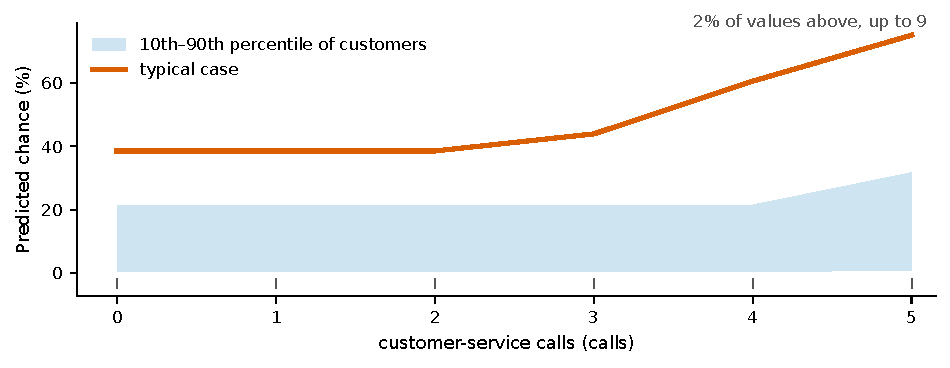
\includegraphics[width=\linewidth,height=0.88\textheight,keepaspectratio]{figures/churn100-s4-c3/ann_83-response.pdf}
\caption{Late rise in calls: Response curves through this part: the typical case (bold), the 10th to 90th percentile of individual customers (band), the fold or step point (dashed) with its spread across them (grey), and the observed values (ticks).}
\label{fig:churn100s4c3:plot-ann83-0}
\end{figure}
\begin{figure}[H]\centering
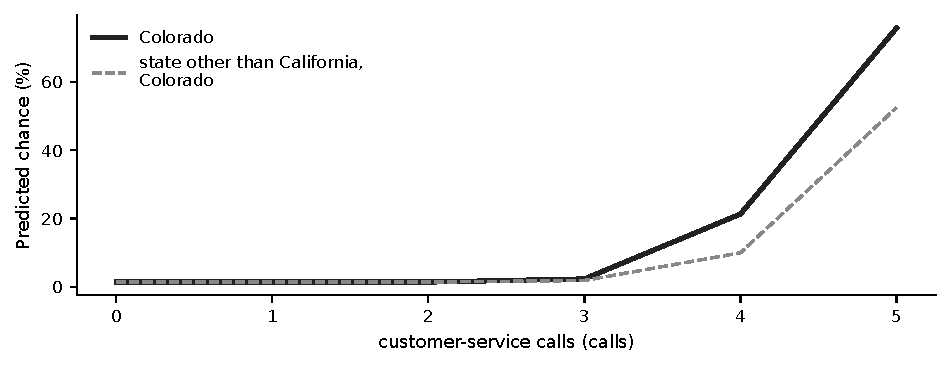
\includegraphics[width=\linewidth,height=0.88\textheight,keepaspectratio]{figures/churn100-s4-c3/ann_83-interaction.pdf}
\caption{Late rise in calls: How the effect differs between groups: one curve per group, for the typical case of each group.}
\label{fig:churn100s4c3:plot-ann83-1}
\end{figure}
\begin{figure}[H]\centering
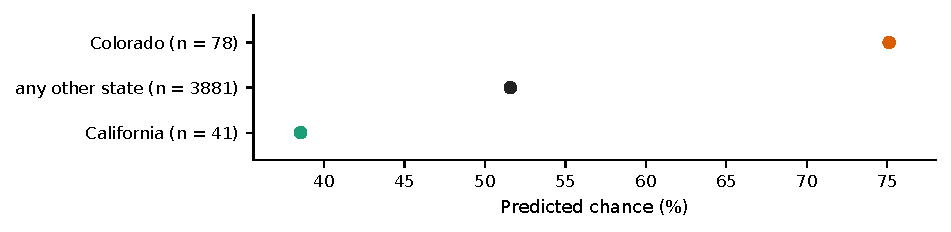
\includegraphics[width=\linewidth,height=0.88\textheight,keepaspectratio]{figures/churn100-s4-c3/ann_83-categories-small.pdf}
\caption{Late rise in calls: The predicted value for the typical case at each level, through this part (n = training customers; grey: fewer than 20).}
\label{fig:churn100s4c3:plot-ann83-2}
\end{figure}
\begin{figure}[H]\centering
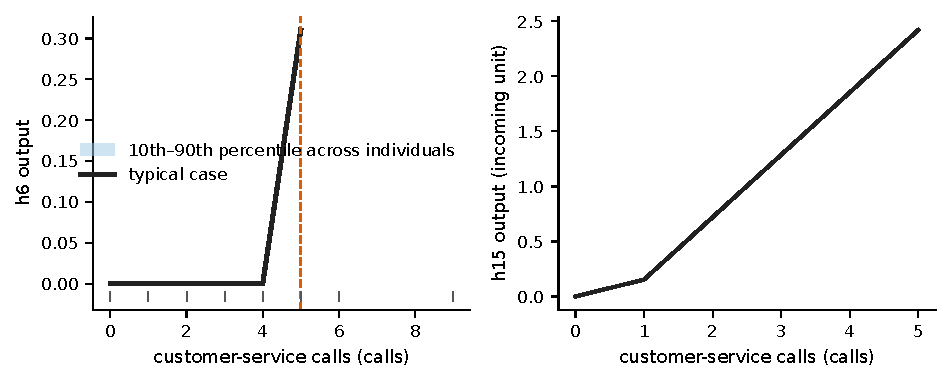
\includegraphics[width=\linewidth,height=0.88\textheight,keepaspectratio]{figures/churn100-s4-c3/ann_83-partial-5268.pdf}
\caption{Late rise in calls: This part's own output, unit h6 (combines 2 non-linear units), on its own scale (its activation), with every other input at the typical case; it is active for 134 of 4000. Bold: the typical case; band: 10th to 90th percentile across individuals; dashed: where it switches on; ticks: the data.}
\label{fig:churn100s4c3:plot-ann83-3}
\end{figure}
\begin{figure}[H]\centering
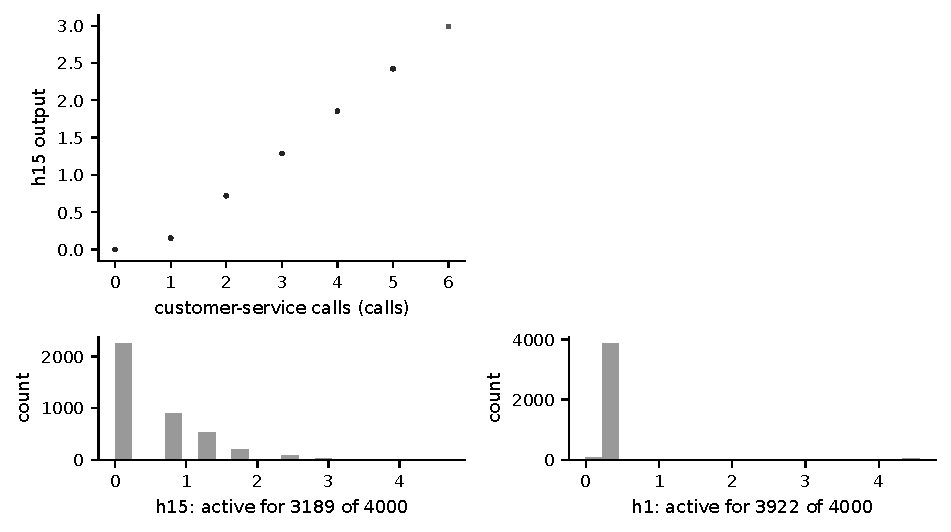
\includegraphics[width=\linewidth,height=0.88\textheight,keepaspectratio]{figures/churn100-s4-c3/ann_83-units.pdf}
\caption{Late rise in calls: This part's hidden units: each unit's output against its main numeric input (top) and how often it is active (bottom).}
\label{fig:churn100s4c3:plot-ann83-4}
\end{figure}
\par\smallskip\noindent{\small Technical detail: \ref{tech:ann83}.\par}
\subsubsection{Heavy daytime use}\label{rd:ann85}
\noindent{\footnotesize Part of: The whole model (\ref{rd:ann88}).\par}
\noindent{\small Figure~\ref{fig:churn100s4c3:parts-ann85} shows what feeds this part; Figure~\ref{fig:churn100s4c3:units-ann85} its units and every connection into them (dashed boxes: connections from or to other parts, drawn in their own sections).\par}
\begin{figure}[H]\centering
\resizebox{!}{\ifdim\height>0.5\textheight 0.5\textheight\else\height\fi}{%
\resizebox{\ifdim\width>\linewidth\linewidth\else\width\fi}{!}{%
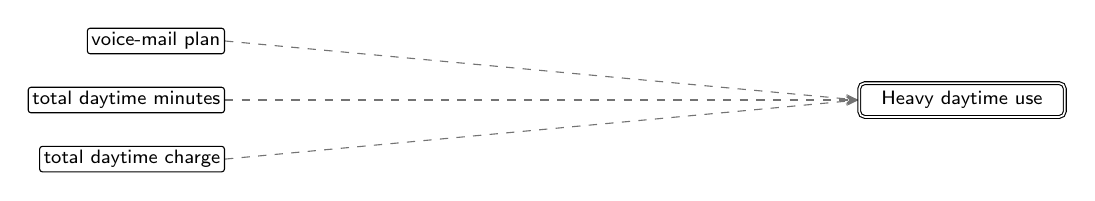
\begin{tikzpicture}[
  font=\sffamily\scriptsize, >={Stealth[length=1.6mm]},
  inp/.style={draw, rounded corners=1pt, fill=white, inner sep=1.5pt, minimum height=3.2mm, anchor=east},
  abox/.style={draw, thick, rounded corners=2pt, align=center, inner sep=3pt, minimum height=6mm, text width=42mm},
  outp/.style={draw, double, rounded corners=2pt, fill=white, align=center, inner sep=3pt, text width=24mm},
  agg/.style={draw=black!55},
]
\node[inp] (i0) at (0,0.75) {voice-mail plan};
\node[inp] (i1) at (0,-0.0) {total daytime minutes};
\node[inp] (i2) at (0,-0.75) {total daytime charge};
\node[outp] (out) at (9.36,0) {Heavy daytime use};
\begin{scope}[on background layer]
\draw[->, agg, thin, dashed] (i0.east) -- (out.west);
\draw[->, agg, thin, dashed] (i1.east) -- (out.west);
\draw[->, agg, thin, dashed] (i2.east) -- (out.west);
\end{scope}
\end{tikzpicture}}}%
\caption{Heavy daytime use: what feeds it, one level down.}
\label{fig:churn100s4c3:parts-ann85}
\end{figure}
\begin{figure}[H]\centering
\resizebox{\ifdim\width>\linewidth\linewidth\else\width\fi}{!}{%
\definecolor{netup}{HTML}{D95F02}\definecolor{netdown}{HTML}{1B9E77}\definecolor{netmixed}{HTML}{7F7F7F}%
\begin{tikzpicture}[
  font=\sffamily\scriptsize, >={Stealth[length=1.4mm]},
  inp/.style={draw, circle, fill=white, minimum size=3.2mm, inner sep=0pt},
  hid/.style={draw, circle, fill=white, minimum size=5.2mm, inner sep=0.5pt, font=\sffamily\tiny},
  exitbox/.style={draw, thick, rectangle, fill=white, align=center, text width=17mm, minimum height=5mm, inner sep=1.5pt, font=\sffamily\tiny},
  sumbox/.style={draw, thick, dashed, rectangle, fill=white, align=center, text width=17mm, minimum height=5mm, inner sep=1.5pt, font=\sffamily\tiny},
  outp/.style={draw, thick, regular polygon, regular polygon sides=6, fill=white, minimum size=10mm, inner sep=0pt, font=\sffamily\tiny, align=center},
  stub/.style={draw, dashed, rounded corners=2pt, fill=white, align=center, inner sep=2pt, font=\sffamily\tiny, text width=15mm},
  inlab/.style={font=\sffamily\tiny, align=center, text width=15mm, inner sep=1pt, fill=white, fill opacity=0.8, text opacity=1},
  wpos/.style={draw=NavyBlue}, wneg/.style={draw=BrickRed}, wagg/.style={draw=black!45, line width=1.2pt},
  wmix/.style={draw=Plum},
]
\node[hid] (n4000) at (4.2,1.9) {h5};
\node[hid] (n3118) at (2.7,1.9) {h4};
\node[hid] (n10131) at (1.2,1.9) {h13};
\node[inp, draw=netup, very thick] (ninxxtotalxdayxminutes) at (4.5,0.0) {};
\path (ninxxtotalxdayxminutes.south) node[inlab, anchor=north] (labninxxtotalxdayxminutes) {total daytime minutes $\uparrow$};
\node[inp] (ninxxtotalxdayxcharge) at (2.7,0.0) {};
\path (ninxxtotalxdayxcharge.south) node[inlab, anchor=north] (labninxxtotalxdayxcharge) {total daytime charge};
\node[inp, draw=netdown, very thick] (ninxxvoicexmailxplan) at (0.9,0.0) {};
\path (ninxxvoicexmailxplan.south) node[inlab, anchor=north] (labninxxvoicexmailxplan) {a voice-mail plan $\downarrow$};
\node[stub] (ntoxxthexmodelxoutput) at (2.7,3.45) {to the model output};
\begin{scope}[on background layer]
\node[fit=(n4000) (n3118) (n10131) , inner sep=8pt, rounded corners=5pt, fill=Orchid!10, draw=Orchid!45] (clu0) {};
\draw[->, wpos, line width=0.50pt] (ninxxtotalxdayxminutes) -- (n4000);
\draw[->, wpos, line width=0.38pt] (ninxxtotalxdayxcharge) -- (n3118);
\draw[->, wpos, line width=0.53pt] (ninxxtotalxdayxminutes) -- (n10131);
\draw[->, wneg, line width=0.37pt] (ninxxvoicexmailxplan) -- (n10131);
\draw[->, wpos, line width=0.77pt] (n3118) -- (ntoxxthexmodelxoutput);
\draw[->, wpos, line width=0.77pt] (n4000) -- (ntoxxthexmodelxoutput);
\draw[->, wpos, line width=0.91pt] (n10131) -- (ntoxxthexmodelxoutput);
\end{scope}
\node[font=\sffamily\scriptsize\bfseries, text=Orchid!55!black, anchor=south west, inner sep=1pt, fill=white, fill opacity=0.85, text opacity=1] at (clu0.north west) {Heavy daytime use};
\end{tikzpicture}}%
\caption{Heavy daytime use: its units and every connection into them. Blue: positive weight (raises the score); red: negative weight (lowers it); thicker: larger weight. Orange outline and up arrow: raises the final prediction; teal and down arrow: lowers it; grey and double arrow: depends.}
\label{fig:churn100s4c3:units-ann85}
\end{figure}
\paragraph{Hypothesis.} This part raises the chance of leaving for heavy daytime users: daytime minutes add to it only above about 209 minutes, in an uneven way, and much less with a voice-mail plan.\,{\scriptsize\textcolor{NavyBlue}{[C100, C099]}}
\paragraph{Evidence.} This part acts on 1074 of 4000 training customers, 290 of whom left; for the typical customer it acts on, the chance is about 1\% without it and about 4\% with it.\,{\scriptsize\textcolor{NavyBlue}{[C102]}} Daytime minutes add to the chance only once they rise above about 209 minutes, in an uneven way: for a typical such customer, from about 1\% at 0 minutes to about 16\% at 271 minutes, flattening out near the bottom because the predicted chance cannot go much lower.\,{\scriptsize\textcolor{NavyBlue}{[C100]}} The rise is much larger without a voice-mail plan: from 112 to 249 daytime minutes the chance goes from about 1\% to about 6\% without one, but stays below 1\% with one, in an uneven way, flattening out near the bottom because the predicted chance cannot go much lower.\,{\scriptsize\textcolor{NavyBlue}{[C099]}} A voice-mail plan lowers it: for the typical customer it acts on, from about 4\% to about 2\%.\,{\scriptsize\textcolor{NavyBlue}{[C098]}} Its formula reproduces the part exactly on all 4000 training customers.\,{\scriptsize\textcolor{NavyBlue}{[C103]}}
\par\noindent{\small Evidence plots: Figure~\ref{fig:churn100s4c3:plot-ann85-0}, Figure~\ref{fig:churn100s4c3:plot-ann85-1}, Figure~\ref{fig:churn100s4c3:plot-ann85-2}, Figure~\ref{fig:churn100s4c3:plot-ann85-3}, Figure~\ref{fig:churn100s4c3:plot-ann85-4}, Figure~\ref{fig:churn100s4c3:plot-ann85-5}.\par}
\par\noindent{\small Figure~\ref{fig:churn100s4c3:plot-ann85-3} shows this part's own output, unit h13: it switches on at about 209 minutes of total daytime minutes, and is zero below.\par}
\par\noindent{\small Figure~\ref{fig:churn100s4c3:plot-ann85-4} shows this part's own output, unit h5: it switches on at about 223.9 minutes of total daytime minutes, and is zero below.\par}
\begin{figure}[H]\centering
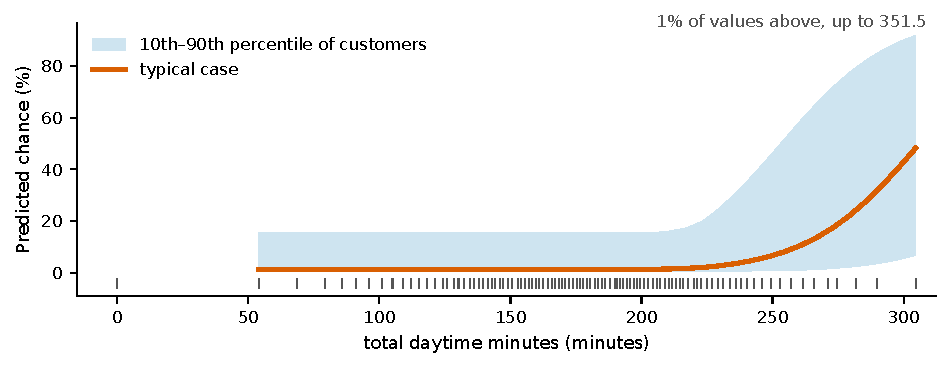
\includegraphics[width=\linewidth,height=0.88\textheight,keepaspectratio]{figures/churn100-s4-c3/ann_85-response.pdf}
\caption{Heavy daytime use: Response curves through this part: the typical case (bold), the 10th to 90th percentile of individual customers (band), the fold or step point (dashed) with its spread across them (grey), and the observed values (ticks).}
\label{fig:churn100s4c3:plot-ann85-0}
\end{figure}
\begin{figure}[H]\centering
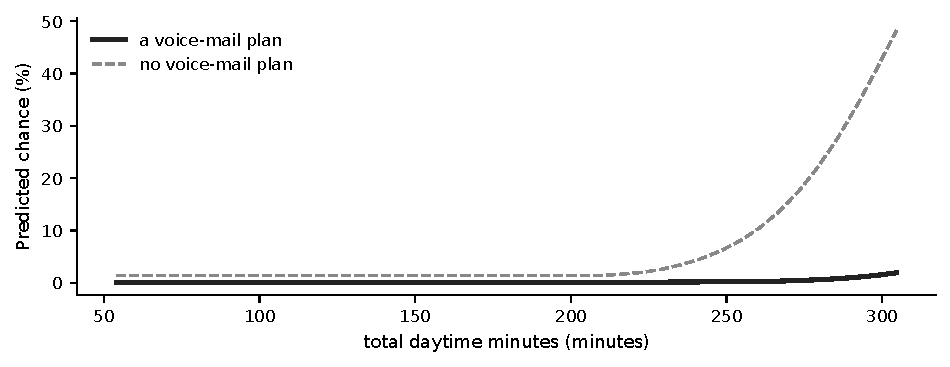
\includegraphics[width=\linewidth,height=0.88\textheight,keepaspectratio]{figures/churn100-s4-c3/ann_85-interaction.pdf}
\caption{Heavy daytime use: How the effect differs between groups: one curve per group, for the typical case of each group.}
\label{fig:churn100s4c3:plot-ann85-1}
\end{figure}
\begin{figure}[H]\centering
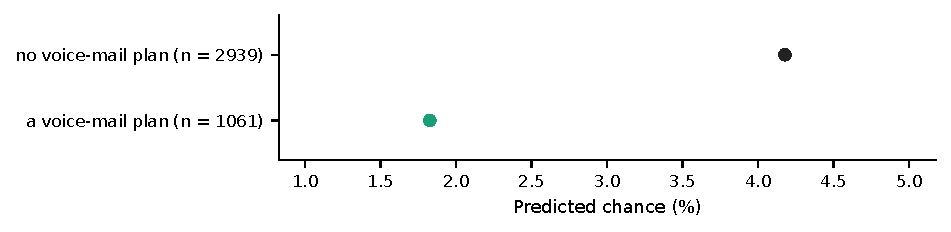
\includegraphics[width=\linewidth,height=0.88\textheight,keepaspectratio]{figures/churn100-s4-c3/ann_85-categories-small.pdf}
\caption{Heavy daytime use: The predicted value for the typical case at each level, through this part (n = training customers; grey: fewer than 20).}
\label{fig:churn100s4c3:plot-ann85-2}
\end{figure}
\begin{figure}[H]\centering
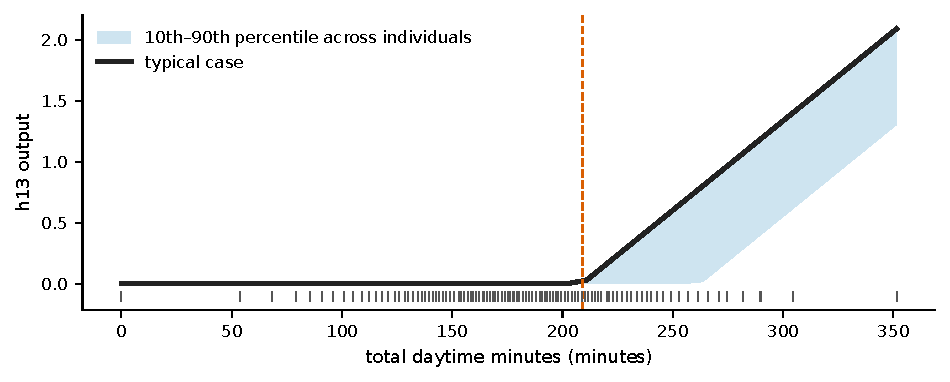
\includegraphics[width=\linewidth,height=0.88\textheight,keepaspectratio]{figures/churn100-s4-c3/ann_85-partial-10131.pdf}
\caption{Heavy daytime use: This part's own output, unit h13 (the output of 'Heavy daytime use'), on its own scale (its activation), with every other input at the typical case; it is active for 929 of 4000. Bold: the typical case; band: 10th to 90th percentile across individuals; dashed: where it switches on; ticks: the data.}
\label{fig:churn100s4c3:plot-ann85-3}
\end{figure}
\begin{figure}[H]\centering
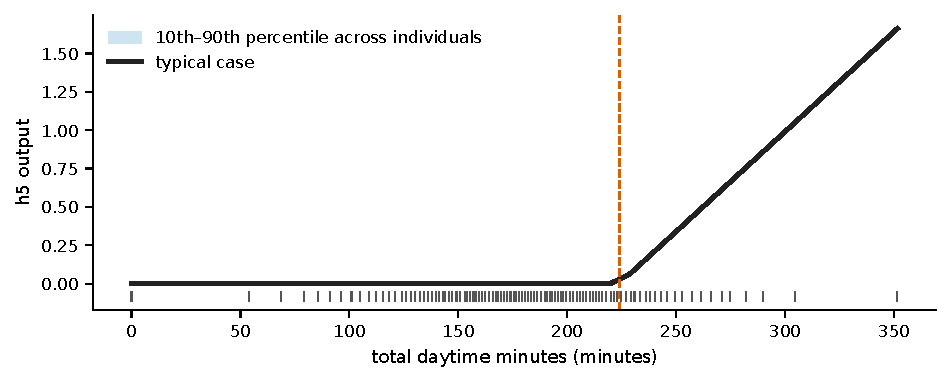
\includegraphics[width=\linewidth,height=0.88\textheight,keepaspectratio]{figures/churn100-s4-c3/ann_85-partial-4000.pdf}
\caption{Heavy daytime use: This part's own output, unit h5 (the output of 'Heavy daytime use'), on its own scale (its activation), with every other input at the typical case; it is active for 818 of 4000. Bold: the typical case; band: 10th to 90th percentile across individuals; dashed: where it switches on; ticks: the data.}
\label{fig:churn100s4c3:plot-ann85-4}
\end{figure}
\begin{figure}[H]\centering
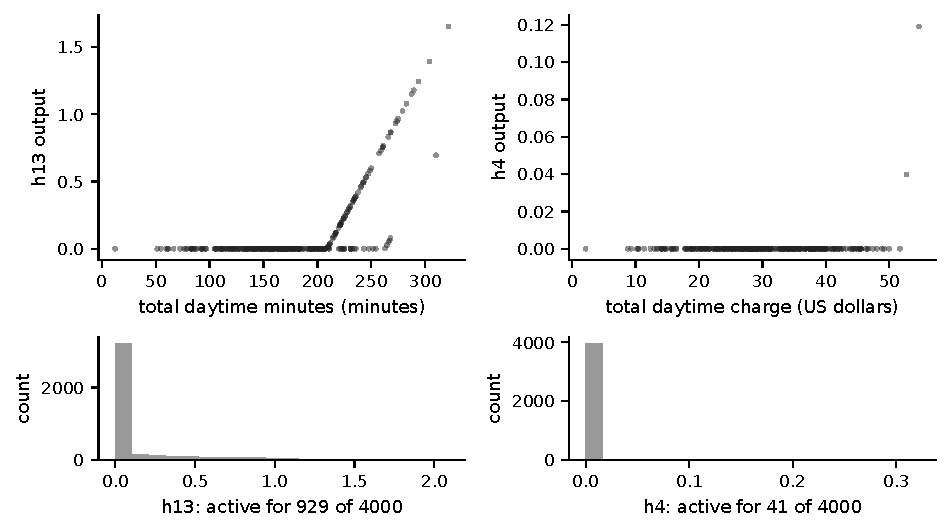
\includegraphics[width=\linewidth,height=0.88\textheight,keepaspectratio]{figures/churn100-s4-c3/ann_85-units.pdf}
\caption{Heavy daytime use: This part's hidden units: each unit's output against its main numeric input (top) and how often it is active (bottom).}
\label{fig:churn100s4c3:plot-ann85-5}
\end{figure}
\par\smallskip\noindent{\small Technical detail: \ref{tech:ann85}.\par}
\subsubsection{State units}\label{rd:ann86}
\noindent{\footnotesize Part of: The whole model (\ref{rd:ann88}).\par}
\noindent{\small Figure~\ref{fig:churn100s4c3:parts-ann86} shows what feeds this part; Figure~\ref{fig:churn100s4c3:units-ann86} its units and every connection into them (dashed boxes: connections from or to other parts, drawn in their own sections).\par}
\begin{figure}[H]\centering
\resizebox{!}{\ifdim\height>0.5\textheight 0.5\textheight\else\height\fi}{%
\resizebox{\ifdim\width>\linewidth\linewidth\else\width\fi}{!}{%
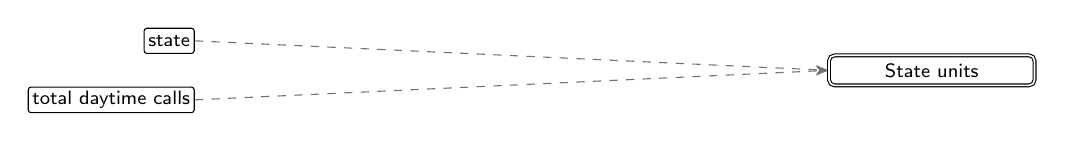
\begin{tikzpicture}[
  font=\sffamily\scriptsize, >={Stealth[length=1.6mm]},
  inp/.style={draw, rounded corners=1pt, fill=white, inner sep=1.5pt, minimum height=3.2mm, anchor=east},
  abox/.style={draw, thick, rounded corners=2pt, align=center, inner sep=3pt, minimum height=6mm, text width=42mm},
  outp/.style={draw, double, rounded corners=2pt, fill=white, align=center, inner sep=3pt, text width=24mm},
  agg/.style={draw=black!55},
]
\node[inp] (i0) at (0,0.375) {state};
\node[inp] (i1) at (0,-0.375) {total daytime calls};
\node[outp] (out) at (9.36,0) {State units};
\begin{scope}[on background layer]
\draw[->, agg, thin, dashed] (i0.east) -- (out.west);
\draw[->, agg, thin, dashed] (i1.east) -- (out.west);
\end{scope}
\end{tikzpicture}}}%
\caption{State units: what feeds it, one level down.}
\label{fig:churn100s4c3:parts-ann86}
\end{figure}
\begin{figure}[H]\centering
\resizebox{\ifdim\width>\linewidth\linewidth\else\width\fi}{!}{%
\definecolor{netup}{HTML}{D95F02}\definecolor{netdown}{HTML}{1B9E77}\definecolor{netmixed}{HTML}{7F7F7F}%
\begin{tikzpicture}[
  font=\sffamily\scriptsize, >={Stealth[length=1.4mm]},
  inp/.style={draw, circle, fill=white, minimum size=3.2mm, inner sep=0pt},
  hid/.style={draw, circle, fill=white, minimum size=5.2mm, inner sep=0.5pt, font=\sffamily\tiny},
  exitbox/.style={draw, thick, rectangle, fill=white, align=center, text width=17mm, minimum height=5mm, inner sep=1.5pt, font=\sffamily\tiny},
  sumbox/.style={draw, thick, dashed, rectangle, fill=white, align=center, text width=17mm, minimum height=5mm, inner sep=1.5pt, font=\sffamily\tiny},
  outp/.style={draw, thick, regular polygon, regular polygon sides=6, fill=white, minimum size=10mm, inner sep=0pt, font=\sffamily\tiny, align=center},
  stub/.style={draw, dashed, rounded corners=2pt, fill=white, align=center, inner sep=2pt, font=\sffamily\tiny, text width=15mm},
  inlab/.style={font=\sffamily\tiny, align=center, text width=15mm, inner sep=1pt, fill=white, fill opacity=0.8, text opacity=1},
  wpos/.style={draw=NavyBlue}, wneg/.style={draw=BrickRed}, wagg/.style={draw=black!45, line width=1.2pt},
  wmix/.style={draw=Plum},
]
\node[hid] (n17102) at (10.85,1.9) {h21};
\node[hid] (n15362) at (7.85,1.9) {h18};
\node[hid] (n9954) at (13.85,1.9) {h12};
\node[hid] (n11361) at (0.35,1.9) {h14};
\node[hid] (n5786) at (12.35,1.9) {h8};
\node[hid] (n15490) at (9.35,1.9) {h19};
\node[hid] (n5533) at (7.1,3.25) {h7};
\node[hid] (n7872) at (8.6,3.25) {h10};
\node[hid] (n1390) at (6.35,1.9) {h3};
\node[hid] (n1295) at (3.35,1.9) {h2};
\node[hid] (n15904) at (5.6,3.25) {h20};
\node[hid] (n12690) at (1.85,1.9) {h16};
\node[hid] (n13068) at (4.85,1.9) {h17};
\node[inp, draw=netmixed, very thick] (ngrpxxstate) at (6.2,0.0) {};
\path (ngrpxxstate.south) node[inlab, anchor=north] (labngrpxxstate) {state (31 of 51 used) $\updownarrow$};
\node[inp, draw=netup, very thick] (ninxxtotalxdayxcalls) at (8.0,0.0) {};
\path (ninxxtotalxdayxcalls.south) node[inlab, anchor=north] (labninxxtotalxdayxcalls) {total daytime calls $\uparrow$};
\node[stub] (ntoxxthexmodelxoutput) at (7.1,4.8) {to the model output};
\begin{scope}[on background layer]
\node[fit=(n17102) (n15362) (n9954) (n11361) (n5786) (n15490) (n5533) (n7872) (n1390) (n1295) (n15904) (n12690) (n13068) , inner sep=8pt, rounded corners=5pt, fill=Goldenrod!10, draw=Goldenrod!45] (clu0) {};
\draw[->, wpos, line width=0.61pt] (n1295) -- (n7872);
\draw[->, wpos, line width=0.48pt] (n5786) -- (n5533);
\draw[->, wpos, line width=0.60pt] (n15490) -- (n15904);
\draw[->, wneg, line width=0.25pt] (ninxxtotalxdayxcalls) -- (n5533);
\draw[->, wneg, line width=0.64pt] (n1295) -- (ntoxxthexmodelxoutput);
\draw[->, wneg, line width=0.66pt] (n1390) -- (ntoxxthexmodelxoutput);
\draw[->, wpos, line width=0.94pt] (n5533) -- (ntoxxthexmodelxoutput);
\draw[->, wneg, line width=0.44pt] (n5786) -- (ntoxxthexmodelxoutput);
\draw[->, wneg, line width=0.69pt] (n7872) -- (ntoxxthexmodelxoutput);
\draw[->, wpos, line width=0.27pt] (n9954) -- (ntoxxthexmodelxoutput);
\draw[->, wpos, line width=0.27pt] (n11361) -- (ntoxxthexmodelxoutput);
\draw[->, wneg, line width=0.26pt] (n12690) -- (ntoxxthexmodelxoutput);
\draw[->, wneg, line width=0.26pt] (n13068) -- (ntoxxthexmodelxoutput);
\draw[->, wpos, line width=0.27pt] (n15362) -- (ntoxxthexmodelxoutput);
\draw[->, wpos, line width=0.26pt] (n15490) -- (ntoxxthexmodelxoutput);
\draw[->, wpos, line width=0.27pt] (n15904) -- (ntoxxthexmodelxoutput);
\draw[->, wneg, line width=0.30pt] (n17102) -- (ntoxxthexmodelxoutput);
\draw[->, wpos, line width=0.60pt] (ngrpxxstate) -- node[pos=0.8, sloped, above, font=\sffamily\tiny, inner sep=1pt, fill=white, fill opacity=0.8, text opacity=1] {+1.01} (n9954);
\draw[->, wneg, line width=0.45pt] (ngrpxxstate) -- node[pos=0.8, sloped, above, font=\sffamily\tiny, inner sep=1pt, fill=white, fill opacity=0.8, text opacity=1] {-0.57} (n1390);
\draw[->, wmix, line width=0.78pt] (ngrpxxstate) -- node[pos=0.8, sloped, above, font=\sffamily\tiny, inner sep=1pt, fill=white, fill opacity=0.8, text opacity=1] {3 edges, -1.50 to +0.16} (n5786);
\draw[->, wpos, line width=0.60pt] (ngrpxxstate) -- node[pos=0.8, sloped, above, font=\sffamily\tiny, inner sep=1pt, fill=white, fill opacity=0.8, text opacity=1] {+1.00} (n15362);
\draw[->, wpos, line width=0.59pt] (ngrpxxstate) -- node[pos=0.8, sloped, above, font=\sffamily\tiny, inner sep=1pt, fill=white, fill opacity=0.8, text opacity=1] {+0.98} (n15490);
\draw[->, wpos, line width=0.60pt] (ngrpxxstate) -- node[pos=0.8, sloped, above, font=\sffamily\tiny, inner sep=1pt, fill=white, fill opacity=0.8, text opacity=1] {+0.99} (n17102);
\draw[->, wpos, line width=0.60pt] (ngrpxxstate) -- node[pos=0.8, sloped, above, font=\sffamily\tiny, inner sep=1pt, fill=white, fill opacity=0.8, text opacity=1] {+1.00} (n12690);
\draw[->, wpos, line width=0.61pt] (ngrpxxstate) -- node[pos=0.8, sloped, above, font=\sffamily\tiny, inner sep=1pt, fill=white, fill opacity=0.8, text opacity=1] {+1.02} (n13068);
\draw[->, wpos, line width=0.83pt] (ngrpxxstate) -- node[pos=0.8, sloped, above, font=\sffamily\tiny, inner sep=1pt, fill=white, fill opacity=0.8, text opacity=1] {+1.65} (n11361);
\draw[->, wneg, line width=0.70pt] (ngrpxxstate) -- node[pos=0.8, sloped, above, font=\sffamily\tiny, inner sep=1pt, fill=white, fill opacity=0.8, text opacity=1] {-1.28} (n1295);
\end{scope}
\node[font=\sffamily\scriptsize\bfseries, text=Goldenrod!55!black, anchor=south west, inner sep=1pt, fill=white, fill opacity=0.85, text opacity=1] at (clu0.north west) {State units};
\end{tikzpicture}}%
\caption{State units: its units and every connection into them. Blue: positive weight (raises the score); red: negative weight (lowers it); thicker: larger weight. Orange outline and up arrow: raises the final prediction; teal and down arrow: lowers it; grey and double arrow: depends.}
\label{fig:churn100s4c3:units-ann86}
\end{figure}
\paragraph{Hypothesis.} This part reads only the state: it raises the chance of leaving in Rhode Island, Vermont and Tennessee, and lowers it in Virginia and Nevada.\,{\scriptsize\textcolor{NavyBlue}{[C104, C105, C106, C107, C108]}}
\paragraph{Evidence.} This part reads only the state: it raises a typical customer's chance from about 1\% to about 12\% in Rhode Island, to about 3\% in Vermont and to about 2\% in Tennessee.\,{\scriptsize\textcolor{NavyBlue}{[C104, C105, C106]}} It lowers the chance to below 1\% in Virginia and in Nevada.\,{\scriptsize\textcolor{NavyBlue}{[C107, C108]}} Its formula reproduces the part exactly on all 4000 training customers.\,{\scriptsize\textcolor{NavyBlue}{[C116]}}
\par\noindent{\small Evidence plots: Figure~\ref{fig:churn100s4c3:plot-ann86-0}, Figure~\ref{fig:churn100s4c3:plot-ann86-1}.\par}
\begin{figure}[H]\centering
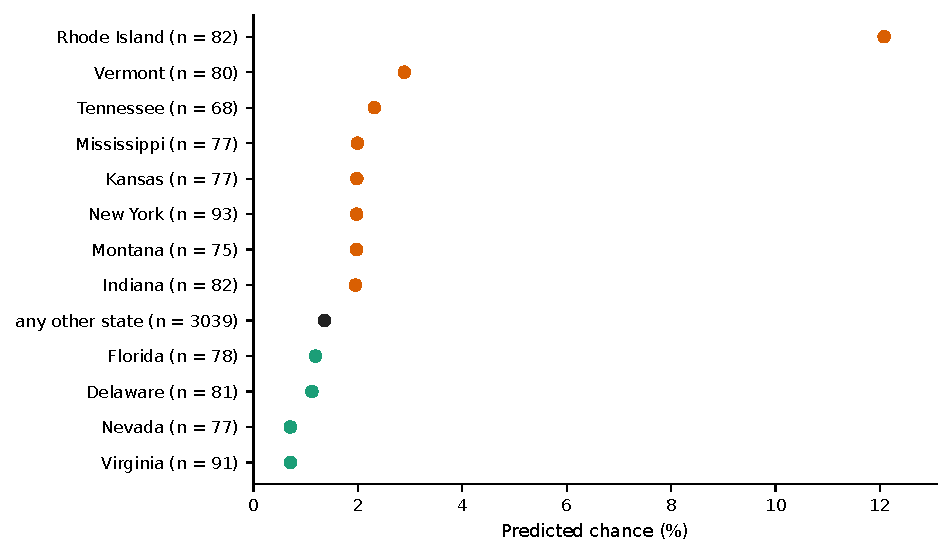
\includegraphics[width=\linewidth,height=0.88\textheight,keepaspectratio]{figures/churn100-s4-c3/ann_86-categories-C104.pdf}
\caption{State units: The predicted value for the typical case at each level, through this part (n = training customers; grey: fewer than 20).}
\label{fig:churn100s4c3:plot-ann86-0}
\end{figure}
\begin{figure}[H]\centering
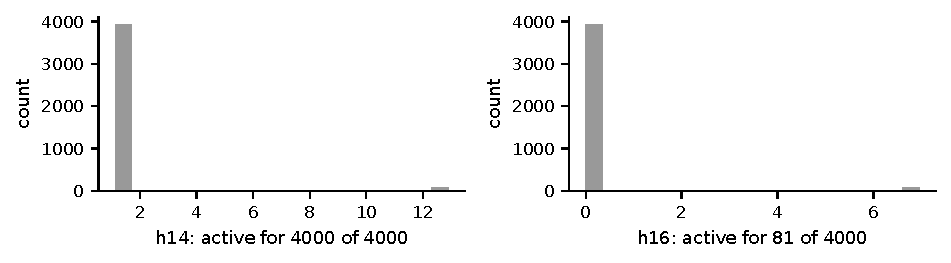
\includegraphics[width=\linewidth,height=0.88\textheight,keepaspectratio]{figures/churn100-s4-c3/ann_86-units.pdf}
\caption{State units: This part's hidden units: each unit's output against its main numeric input (top) and how often it is active (bottom).}
\label{fig:churn100s4c3:plot-ann86-1}
\end{figure}
\par\smallskip\noindent{\small Technical detail: \ref{tech:ann86}.\par}
\subsection{Not supported by the model}
\begin{itemize}\setlength\itemsep{0pt}\small
\item C101: threshold claim about total daytime charge in part ann\_\allowbreak{}85: not supported by the model (the effect past the fold is too small or not consistent across patients).
\item C121: threshold claim about number of calls to customer service in part ann\_\allowbreak{}83: not supported by the model (the effect past the fold is too small or not consistent across patients).
\end{itemize}
\clearpage\section*{Technical detail: churn100-s4-c3}
\addcontentsline{toc}{section}{Technical detail: churn100-s4-c3}
\noindent{\small The record behind each part: the original hypothesis, the closed form, and every claim with its estimate (log-odds and odds ratio), range across patients, n and test check.\par}
\renewcommand{\thesubsection}{T.\arabic{subsection}}\setcounter{subsection}{0}
\subsection{The whole model}\label{tech:ann88}
\noindent{\footnotesize Annotation ann\_\allowbreak{}88 (churn\_\allowbreak{}logit). Reads: state, account length, area code, international calling plan, voice-mail plan, number of voice-mail messages, total daytime minutes, total daytime calls, total daytime charge, total evening minutes, total evening calls, total evening charge, total night-time minutes, total night-time calls, total night-time charge, total international minutes, total international calls, total international charge, number of calls to customer service.\par}
\paragraph{Original hypothesis (unchanged).} Root: logit P(churn) = -1.35 + linear\_\allowbreak{}backbone (identity\_\allowbreak{}lin) + service\_\allowbreak{}calls (identity\_\allowbreak{}svc) + 1.48*3118 + 1.50*4000 + 1.89*10131 (day\_\allowbreak{}usage\_\allowbreak{}hinges) + the state\_\allowbreak{}offsets units (-1.11*1295 - 1.25*7872 - 1.17*1390 - 0.56*5786 + small terms; 5533 is never active), purely additive in the logit; the sigmoid is the only coupling. 30 inputs are unconnected (international minutes, calls and charge, night minutes/\allowbreak{}charge/\allowbreak{}calls,\allowbreak{} evening minutes and calls, area codes 408/510 and 20 state indicators) and have zero effect. Train AUC 0.8884, accuracy 0.8795; the mean predicted churn is 0.082 against a base rate of 0.1415 (the model ranks well but under-predicts). Performance sources (train): all children replaced by least-squares linear fits gives AUC 0.8352 (an L2 logistic regression refit on all 71 inputs gets 0.8433); restoring day\_\allowbreak{}usage\_\allowbreak{}hinges alone gives 0.8713, service\_\allowbreak{}calls alone 0.8657, both 0.8884; the state units restore nothing (exactly linear). So the gain over linear (+0.053) comes from the day-usage and service-call thresholds, which are complementary. Rare-category switches: state:11 -2.50 logit (73 rows, empirical -1.35); state:46 -1.46 net (80 rows, -0.91); state:47 +1.35 (72 rows, +0.92); state:0 -0.97 (56, -0.76); state:14 -0.94 (68, -0.53); state:29 -0.53 direct plus switching off the early service-call hinge (mean -0.78, down to -6.15 for many-call customers; 72 rows, -0.79); state:39 -0.55 net (82, -0.93: direct -2.85 mostly cancelled by the state units); state:33 +0.38 net (direct +1.05, unit -0.68); state:18 +0.36 (65 rows, empirical -0.48: opposite sign); state:4 switches off the late chain (41 rows, empirical +0.80).
\paragraph{Closed form.} Read through its parts (their formulas are in their own sections).
\paragraph{Split inputs.} To annotate the parts, the explanation split these inputs into copies (a refactoring step that does not change what the model computes); the diagrams draw each input once: customer-service calls (2 copies); total daytime calls (2 copies); a voice-mail plan (2 copies).
\paragraph{State: every level the model reads.} Whole-model change in the predicted chance for a typical customer when only the state changes from the reference; n = training customers in that level.\par\smallskip
{\scriptsize\rowcolors{2}{black!6}{white}
\begin{longtable}{@{}lllrlc@{}}
\toprule\rowcolor{white}
Claim & From & To & n & Chance & OK \\
\midrule\endhead
\bottomrule\endfoot
C004 & state other than Alaska, Georgia, Hawaii, Illinois, Indiana, Kansas, Louisiana, Massachusetts, Maine, Mississippi, Montana, North Carolina, North Dakota, Nebraska, Arizona, Nevada, New York, Oklahoma, Oregon, Pennsylvania, Rhode Island, California, South Carolina, Tennessee, Utah, Virginia, Vermont, Washington, Colorado, Delaware, Florida & Washington & 72 & 1\% to 5\% & \textcolor{OliveGreen}{yes} \\
C006 & state other than Alaska, Georgia, Hawaii, Illinois, Indiana, Kansas, Louisiana, Massachusetts, Maine, Mississippi, Montana, North Carolina, North Dakota, Nebraska, Arizona, Nevada, New York, Oklahoma, Oregon, Pennsylvania, Rhode Island, California, South Carolina, Tennessee, Utah, Virginia, Vermont, Washington, Colorado, Delaware, Florida & Maine & 86 & 1\% to 3\% & \textcolor{OliveGreen}{yes} \\
C010 & state other than Alaska, Georgia, Hawaii, Illinois, Indiana, Kansas, Louisiana, Massachusetts, Maine, Mississippi, Montana, North Carolina, North Dakota, Nebraska, Arizona, Nevada, New York, Oklahoma, Oregon, Pennsylvania, Rhode Island, California, South Carolina, Tennessee, Utah, Virginia, Vermont, Washington, Colorado, Delaware, Florida & Tennessee & 68 & 1\% to 2\% & \textcolor{OliveGreen}{yes} \\
C011 & state other than Alaska, Georgia, Hawaii, Illinois, Indiana, Kansas, Louisiana, Massachusetts, Maine, Mississippi, Montana, North Carolina, North Dakota, Nebraska, Arizona, Nevada, New York, Oklahoma, Oregon, Pennsylvania, Rhode Island, California, South Carolina, Tennessee, Utah, Virginia, Vermont, Washington, Colorado, Delaware, Florida & South Carolina & 66 & 1\% to 2\% & \textcolor{OliveGreen}{yes} \\
C017 & state other than Alaska, Georgia, Hawaii, Illinois, Indiana, Kansas, Louisiana, Massachusetts, Maine, Mississippi, Montana, North Carolina, North Dakota, Nebraska, Arizona, Nevada, New York, Oklahoma, Oregon, Pennsylvania, Rhode Island, California, South Carolina, Tennessee, Utah, Virginia, Vermont, Washington, Colorado, Delaware, Florida & Mississippi & 77 & 1\% to 2\% & \textcolor{OliveGreen}{yes} \\
C018 & state other than Alaska, Georgia, Hawaii, Illinois, Indiana, Kansas, Louisiana, Massachusetts, Maine, Mississippi, Montana, North Carolina, North Dakota, Nebraska, Arizona, Nevada, New York, Oklahoma, Oregon, Pennsylvania, Rhode Island, California, South Carolina, Tennessee, Utah, Virginia, Vermont, Washington, Colorado, Delaware, Florida & Nevada & 77 & 1\% to 2\% & \textcolor{OliveGreen}{yes} \\
C019 & state other than Alaska, Georgia, Hawaii, Illinois, Indiana, Kansas, Louisiana, Massachusetts, Maine, Mississippi, Montana, North Carolina, North Dakota, Nebraska, Arizona, Nevada, New York, Oklahoma, Oregon, Pennsylvania, Rhode Island, California, South Carolina, Tennessee, Utah, Virginia, Vermont, Washington, Colorado, Delaware, Florida & Kansas & 77 & 1\% to 2\% & \textcolor{OliveGreen}{yes} \\
C020 & state other than Alaska, Georgia, Hawaii, Illinois, Indiana, Kansas, Louisiana, Massachusetts, Maine, Mississippi, Montana, North Carolina, North Dakota, Nebraska, Arizona, Nevada, New York, Oklahoma, Oregon, Pennsylvania, Rhode Island, California, South Carolina, Tennessee, Utah, Virginia, Vermont, Washington, Colorado, Delaware, Florida & Montana & 75 & 1\% to 2\% & \textcolor{OliveGreen}{yes} \\
C021 & state other than Alaska, Georgia, Hawaii, Illinois, Indiana, Kansas, Louisiana, Massachusetts, Maine, Mississippi, Montana, North Carolina, North Dakota, Nebraska, Arizona, Nevada, New York, Oklahoma, Oregon, Pennsylvania, Rhode Island, California, South Carolina, Tennessee, Utah, Virginia, Vermont, Washington, Colorado, Delaware, Florida & New York & 93 & 1\% to 2\% & \textcolor{OliveGreen}{yes} \\
C022 & state other than Alaska, Georgia, Hawaii, Illinois, Indiana, Kansas, Louisiana, Massachusetts, Maine, Mississippi, Montana, North Carolina, North Dakota, Nebraska, Arizona, Nevada, New York, Oklahoma, Oregon, Pennsylvania, Rhode Island, California, South Carolina, Tennessee, Utah, Virginia, Vermont, Washington, Colorado, Delaware, Florida & Indiana & 82 & 1\% to 2\% & \textcolor{OliveGreen}{yes} \\
C023 & state other than Alaska, Georgia, Hawaii, Illinois, Indiana, Kansas, Louisiana, Massachusetts, Maine, Mississippi, Montana, North Carolina, North Dakota, Nebraska, Arizona, Nevada, New York, Oklahoma, Oregon, Pennsylvania, Rhode Island, California, South Carolina, Tennessee, Utah, Virginia, Vermont, Washington, Colorado, Delaware, Florida & Louisiana & 65 & 1\% to 2\% & \textcolor{OliveGreen}{yes} \\
C024 & state other than Alaska, Georgia, Hawaii, Illinois, Indiana, Kansas, Louisiana, Massachusetts, Maine, Mississippi, Montana, North Carolina, North Dakota, Nebraska, Arizona, Nevada, New York, Oklahoma, Oregon, Pennsylvania, Rhode Island, California, South Carolina, Tennessee, Utah, Virginia, Vermont, Washington, Colorado, Delaware, Florida & Utah & 89 & 1\% to 2\% & \textcolor{OliveGreen}{yes} \\
C026 & state other than Alaska, Georgia, Hawaii, Illinois, Indiana, Kansas, Louisiana, Massachusetts, Maine, Mississippi, Montana, North Carolina, North Dakota, Nebraska, Arizona, Nevada, New York, Oklahoma, Oregon, Pennsylvania, Rhode Island, California, South Carolina, Tennessee, Utah, Virginia, Vermont, Washington, Colorado, Delaware, Florida & Massachusetts & 86 & 1\% to 2\% & \textcolor{OliveGreen}{yes} \\
C032 & state other than Alaska, Georgia, Hawaii, Illinois, Indiana, Kansas, Louisiana, Massachusetts, Maine, Mississippi, Montana, North Carolina, North Dakota, Nebraska, Arizona, Nevada, New York, Oklahoma, Oregon, Pennsylvania, Rhode Island, California, South Carolina, Tennessee, Utah, Virginia, Vermont, Washington, Colorado, Delaware, Florida & Oregon & 84 & 1\% to 2\% & \textcolor{OliveGreen}{yes} \\
C035 & state other than Alaska, Georgia, Hawaii, Illinois, Indiana, Kansas, Louisiana, Massachusetts, Maine, Mississippi, Montana, North Carolina, North Dakota, Nebraska, Arizona, Nevada, New York, Oklahoma, Oregon, Pennsylvania, Rhode Island, California, South Carolina, Tennessee, Utah, Virginia, Vermont, Washington, Colorado, Delaware, Florida & North Dakota & 68 & 1\% to 1\% & \textcolor{OliveGreen}{yes} \\
C036 & state other than Alaska, Georgia, Hawaii, Illinois, Indiana, Kansas, Louisiana, Massachusetts, Maine, Mississippi, Montana, North Carolina, North Dakota, Nebraska, Arizona, Nevada, New York, Oklahoma, Oregon, Pennsylvania, Rhode Island, California, South Carolina, Tennessee, Utah, Virginia, Vermont, Washington, Colorado, Delaware, Florida & Oklahoma & 79 & 1\% to 1\% & \textcolor{OliveGreen}{yes} \\
C039 & state other than Alaska, Georgia, Hawaii, Illinois, Indiana, Kansas, Louisiana, Massachusetts, Maine, Mississippi, Montana, North Carolina, North Dakota, Nebraska, Arizona, Nevada, New York, Oklahoma, Oregon, Pennsylvania, Rhode Island, California, South Carolina, Tennessee, Utah, Virginia, Vermont, Washington, Colorado, Delaware, Florida & California & 41 & 1\% to 1\% & \textcolor{OliveGreen}{yes} \\
C040 & state other than Alaska, Georgia, Hawaii, Illinois, Indiana, Kansas, Louisiana, Massachusetts, Maine, Mississippi, Montana, North Carolina, North Dakota, Nebraska, Arizona, Nevada, New York, Oklahoma, Oregon, Pennsylvania, Rhode Island, California, South Carolina, Tennessee, Utah, Virginia, Vermont, Washington, Colorado, Delaware, Florida & Colorado & 78 & 1\% to 1\% & \textcolor{OliveGreen}{yes} \\
C037 & state other than Alaska, Georgia, Hawaii, Illinois, Indiana, Kansas, Louisiana, Massachusetts, Maine, Mississippi, Montana, North Carolina, North Dakota, Nebraska, Arizona, Nevada, New York, Oklahoma, Oregon, Pennsylvania, Rhode Island, California, South Carolina, Tennessee, Utah, Virginia, Vermont, Washington, Colorado, Delaware, Florida & Arizona & 73 & 1\% to 1\% & \textcolor{OliveGreen}{yes} \\
C034 & state other than Alaska, Georgia, Hawaii, Illinois, Indiana, Kansas, Louisiana, Massachusetts, Maine, Mississippi, Montana, North Carolina, North Dakota, Nebraska, Arizona, Nevada, New York, Oklahoma, Oregon, Pennsylvania, Rhode Island, California, South Carolina, Tennessee, Utah, Virginia, Vermont, Washington, Colorado, Delaware, Florida & North Carolina & 74 & 1\% to 1\% & \textcolor{OliveGreen}{yes} \\
C033 & state other than Alaska, Georgia, Hawaii, Illinois, Indiana, Kansas, Louisiana, Massachusetts, Maine, Mississippi, Montana, North Carolina, North Dakota, Nebraska, Arizona, Nevada, New York, Oklahoma, Oregon, Pennsylvania, Rhode Island, California, South Carolina, Tennessee, Utah, Virginia, Vermont, Washington, Colorado, Delaware, Florida & Delaware & 81 & 1\% to 1\% & \textcolor{OliveGreen}{yes} \\
C028 & state other than Alaska, Georgia, Hawaii, Illinois, Indiana, Kansas, Louisiana, Massachusetts, Maine, Mississippi, Montana, North Carolina, North Dakota, Nebraska, Arizona, Nevada, New York, Oklahoma, Oregon, Pennsylvania, Rhode Island, California, South Carolina, Tennessee, Utah, Virginia, Vermont, Washington, Colorado, Delaware, Florida & Florida & 78 & 1\% to 1\% & \textcolor{OliveGreen}{yes} \\
C027 & state other than Alaska, Georgia, Hawaii, Illinois, Indiana, Kansas, Louisiana, Massachusetts, Maine, Mississippi, Montana, North Carolina, North Dakota, Nebraska, Arizona, Nevada, New York, Oklahoma, Oregon, Pennsylvania, Rhode Island, California, South Carolina, Tennessee, Utah, Virginia, Vermont, Washington, Colorado, Delaware, Florida & Nebraska & 72 & 1\% to 1\% & \textcolor{OliveGreen}{yes} \\
C025 & state other than Alaska, Georgia, Hawaii, Illinois, Indiana, Kansas, Louisiana, Massachusetts, Maine, Mississippi, Montana, North Carolina, North Dakota, Nebraska, Arizona, Nevada, New York, Oklahoma, Oregon, Pennsylvania, Rhode Island, California, South Carolina, Tennessee, Utah, Virginia, Vermont, Washington, Colorado, Delaware, Florida & Rhode Island & 82 & 1\% to 1\% & \textcolor{OliveGreen}{yes} \\
C016 & state other than Alaska, Georgia, Hawaii, Illinois, Indiana, Kansas, Louisiana, Massachusetts, Maine, Mississippi, Montana, North Carolina, North Dakota, Nebraska, Arizona, Nevada, New York, Oklahoma, Oregon, Pennsylvania, Rhode Island, California, South Carolina, Tennessee, Utah, Virginia, Vermont, Washington, Colorado, Delaware, Florida & Georgia & 60 & 1\% to 1\% & \textcolor{OliveGreen}{yes} \\
C015 & state other than Alaska, Georgia, Hawaii, Illinois, Indiana, Kansas, Louisiana, Massachusetts, Maine, Mississippi, Montana, North Carolina, North Dakota, Nebraska, Arizona, Nevada, New York, Oklahoma, Oregon, Pennsylvania, Rhode Island, California, South Carolina, Tennessee, Utah, Virginia, Vermont, Washington, Colorado, Delaware, Florida & Virginia & 91 & 1\% to 1\% & \textcolor{OliveGreen}{yes} \\
C014 & state other than Alaska, Georgia, Hawaii, Illinois, Indiana, Kansas, Louisiana, Massachusetts, Maine, Mississippi, Montana, North Carolina, North Dakota, Nebraska, Arizona, Nevada, New York, Oklahoma, Oregon, Pennsylvania, Rhode Island, California, South Carolina, Tennessee, Utah, Virginia, Vermont, Washington, Colorado, Delaware, Florida & Pennsylvania & 56 & 1\% to 1\% & \textcolor{OliveGreen}{yes} \\
C013 & state other than Alaska, Georgia, Hawaii, Illinois, Indiana, Kansas, Louisiana, Massachusetts, Maine, Mississippi, Montana, North Carolina, North Dakota, Nebraska, Arizona, Nevada, New York, Oklahoma, Oregon, Pennsylvania, Rhode Island, California, South Carolina, Tennessee, Utah, Virginia, Vermont, Washington, Colorado, Delaware, Florida & Illinois & 68 & 1\% to 1\% & \textcolor{OliveGreen}{yes} \\
C012 & state other than Alaska, Georgia, Hawaii, Illinois, Indiana, Kansas, Louisiana, Massachusetts, Maine, Mississippi, Montana, North Carolina, North Dakota, Nebraska, Arizona, Nevada, New York, Oklahoma, Oregon, Pennsylvania, Rhode Island, California, South Carolina, Tennessee, Utah, Virginia, Vermont, Washington, Colorado, Delaware, Florida & Alaska & 56 & 1\% to 1\% & \textcolor{OliveGreen}{yes} \\
C009 & state other than Alaska, Georgia, Hawaii, Illinois, Indiana, Kansas, Louisiana, Massachusetts, Maine, Mississippi, Montana, North Carolina, North Dakota, Nebraska, Arizona, Nevada, New York, Oklahoma, Oregon, Pennsylvania, Rhode Island, California, South Carolina, Tennessee, Utah, Virginia, Vermont, Washington, Colorado, Delaware, Florida & Vermont & 80 & 1\% to $<$1\% & \textcolor{OliveGreen}{yes} \\
C007 & state other than Alaska, Georgia, Hawaii, Illinois, Indiana, Kansas, Louisiana, Massachusetts, Maine, Mississippi, Montana, North Carolina, North Dakota, Nebraska, Arizona, Nevada, New York, Oklahoma, Oregon, Pennsylvania, Rhode Island, California, South Carolina, Tennessee, Utah, Virginia, Vermont, Washington, Colorado, Delaware, Florida & Hawaii & 73 & 1\% to $<$1\% & \textcolor{OliveGreen}{yes} \\
\end{longtable}}
\paragraph{Evidence table} (next page, landscape).
\begin{landscape}
{\scriptsize\setlength{\tabcolsep}{3pt}\renewcommand{\arraystretch}{1.15}
\rowcolors{2}{black!6}{white}
\begin{longtable}{@{}l>{\raggedright\arraybackslash}p{0.36\linewidth}>{\raggedright\arraybackslash}p{0.14\linewidth}rrr>{\raggedright\arraybackslash}p{0.06\linewidth}>{\raggedright\arraybackslash}p{0.17\linewidth}c@{}}
\toprule\rowcolor{white}
ID & What is checked & Risk, typical patient & Log-odds & OR & Range (p10--p90) & n & Test check & OK \\
\midrule\endfirsthead
\toprule\rowcolor{white}
ID & What is checked & Risk, typical patient & Log-odds & OR & Range (p10--p90) & n & Test check & OK \\
\midrule\endhead
\bottomrule\endfoot
C001 & direction: international calling plan: no international plan to an international plan (whole model) \newline{\itshape shape: categorical; highest to lowest: an international plan, no international plan} & 1\% to 18\% & 2.74 & 15.6 & 2.74 to 2.74 & 3620, 380 & agrees; AUC gain 0.066 [0.035, 0.098] & \textcolor{OliveGreen}{yes} \\
C002 & direction: voice-mail messages: 0 messages to 32 messages (whole model) \newline{\itshape shape: steady; 100\% of patients same; verified; risk saturates near 0\%} & 1\% to 6\% & 1.61 & 5.00 & 1.61 to 1.61 & 4000 & agrees; AUC gain 0.014 [0.0002, 0.029] & \textcolor{OliveGreen}{yes} \\
C003 & direction: total daytime minutes: 112 minutes to 249 minutes (whole model) \newline{\itshape shape: accelerating; 100\% of patients same; fallback; risk saturates near 0\%} & 1\% to 6\% & 1.30 & 3.67 & 0.49 to 1.59 & 4000 & agrees; AUC gain 0.074 [0.044, 0.105] & \textcolor{OliveGreen}{yes} \\
C004 & direction: state: state other than Alaska, Georgia, Hawaii, Illinois, Indiana, Kansas, Louisiana, Massachusetts, Maine, Mississippi, Montana, North Carolina, North Dakota, Nebraska, Arizona, Nevada, New York, Oklahoma, Oregon, Pennsylvania, Rhode Island, California, South Carolina, Tennessee, Utah, Virginia, Vermont, Washington, Colorado, Delaware, Florida to Washington (whole model) \newline{\itshape shape: categorical; highest to lowest: Washington, Maine, Tennessee, South Carolina, Mississippi, Nevada ...} & 1\% to 5\% & 1.35 & 3.86 & 1.35 to 1.35 & 1693, 72 & disagrees; AUC gain -0.013 [-0.028, -0.0007] & \textcolor{OliveGreen}{yes} \\
C005 & direction: total evening charge: 11.76 US dollars to 22.57 US dollars (whole model) \newline{\itshape shape: steady; 100\% of patients same; verified; risk saturates near 0\%} & 1\% to 2\% & 1.01 & 2.73 & 1.01 to 1.01 & 4000 & agrees; AUC gain 0.014 [0.003, 0.026] & \textcolor{OliveGreen}{yes} \\
C006 & direction: state: state other than Alaska, Georgia, Hawaii, Illinois, Indiana, Kansas, Louisiana, Massachusetts, Maine, Mississippi, Montana, North Carolina, North Dakota, Nebraska, Arizona, Nevada, New York, Oklahoma, Oregon, Pennsylvania, Rhode Island, California, South Carolina, Tennessee, Utah, Virginia, Vermont, Washington, Colorado, Delaware, Florida to Maine (whole model) \newline{\itshape shape: categorical; highest to lowest: Washington, Maine, Tennessee, South Carolina, Mississippi, Nevada ...} & 1\% to 3\% & 0.71 & 2.04 & 0.71 to 0.71 & 1693, 86 & disagrees; AUC gain -0.013 [-0.028, -0.0007] & \textcolor{OliveGreen}{yes} \\
C007 & direction: state: state other than Alaska, Georgia, Hawaii, Illinois, Indiana, Kansas, Louisiana, Massachusetts, Maine, Mississippi, Montana, North Carolina, North Dakota, Nebraska, Arizona, Nevada, New York, Oklahoma, Oregon, Pennsylvania, Rhode Island, California, South Carolina, Tennessee, Utah, Virginia, Vermont, Washington, Colorado, Delaware, Florida to Hawaii (whole model) \newline{\itshape shape: categorical; highest to lowest: Washington, Maine, Tennessee, South Carolina, Mississippi, Nevada ...} & 1\% to $<$1\% & -2.50 & 0.08 & -2.50 to -2.50 & 1693, 73 & disagrees; AUC gain -0.013 [-0.028, -0.0007] & \textcolor{OliveGreen}{yes} \\
C008 & direction: voice-mail plan: no voice-mail plan to a voice-mail plan (whole model) \newline{\itshape shape: categorical; highest to lowest: no voice-mail plan, a voice-mail plan} & 1\% to $<$1\% & -2.62 & 0.07 & -3.50 to -2.38 & 2939, 1061 & agrees; AUC gain 0.049 [0.028, 0.072] & \textcolor{OliveGreen}{yes} \\
C009 & direction: state: state other than Alaska, Georgia, Hawaii, Illinois, Indiana, Kansas, Louisiana, Massachusetts, Maine, Mississippi, Montana, North Carolina, North Dakota, Nebraska, Arizona, Nevada, New York, Oklahoma, Oregon, Pennsylvania, Rhode Island, California, South Carolina, Tennessee, Utah, Virginia, Vermont, Washington, Colorado, Delaware, Florida to Vermont (whole model) \newline{\itshape shape: categorical; highest to lowest: Washington, Maine, Tennessee, South Carolina, Mississippi, Nevada ...} & 1\% to $<$1\% & -1.46 & 0.23 & -1.46 to -1.46 & 1693, 80 & disagrees; AUC gain -0.013 [-0.028, -0.0007] & \textcolor{OliveGreen}{yes} \\
C010 & direction: state: state other than Alaska, Georgia, Hawaii, Illinois, Indiana, Kansas, Louisiana, Massachusetts, Maine, Mississippi, Montana, North Carolina, North Dakota, Nebraska, Arizona, Nevada, New York, Oklahoma, Oregon, Pennsylvania, Rhode Island, California, South Carolina, Tennessee, Utah, Virginia, Vermont, Washington, Colorado, Delaware, Florida to Tennessee (whole model) \newline{\itshape shape: categorical; highest to lowest: Washington, Maine, Tennessee, South Carolina, Mississippi, Nevada ...} & 1\% to 2\% & 0.54 & 1.72 & 0.54 to 0.54 & 1693, 68 & disagrees; AUC gain -0.013 [-0.028, -0.0007] & \textcolor{OliveGreen}{yes} \\
C011 & direction: state: state other than Alaska, Georgia, Hawaii, Illinois, Indiana, Kansas, Louisiana, Massachusetts, Maine, Mississippi, Montana, North Carolina, North Dakota, Nebraska, Arizona, Nevada, New York, Oklahoma, Oregon, Pennsylvania, Rhode Island, California, South Carolina, Tennessee, Utah, Virginia, Vermont, Washington, Colorado, Delaware, Florida to South Carolina (whole model) \newline{\itshape shape: categorical; highest to lowest: Washington, Maine, Tennessee, South Carolina, Mississippi, Nevada ...} & 1\% to 2\% & 0.54 & 1.71 & 0.54 to 0.54 & 1693, 66 & disagrees; AUC gain -0.013 [-0.028, -0.0007] & \textcolor{OliveGreen}{yes} \\
C012 & direction: state: state other than Alaska, Georgia, Hawaii, Illinois, Indiana, Kansas, Louisiana, Massachusetts, Maine, Mississippi, Montana, North Carolina, North Dakota, Nebraska, Arizona, Nevada, New York, Oklahoma, Oregon, Pennsylvania, Rhode Island, California, South Carolina, Tennessee, Utah, Virginia, Vermont, Washington, Colorado, Delaware, Florida to Alaska (whole model) \newline{\itshape shape: categorical; highest to lowest: Washington, Maine, Tennessee, South Carolina, Mississippi, Nevada ...} & 1\% to 1\% & -0.97 & 0.38 & -0.97 to -0.97 & 1693, 56 & disagrees; AUC gain -0.013 [-0.028, -0.0007] & \textcolor{OliveGreen}{yes} \\
C013 & direction: state: state other than Alaska, Georgia, Hawaii, Illinois, Indiana, Kansas, Louisiana, Massachusetts, Maine, Mississippi, Montana, North Carolina, North Dakota, Nebraska, Arizona, Nevada, New York, Oklahoma, Oregon, Pennsylvania, Rhode Island, California, South Carolina, Tennessee, Utah, Virginia, Vermont, Washington, Colorado, Delaware, Florida to Illinois (whole model) \newline{\itshape shape: categorical; highest to lowest: Washington, Maine, Tennessee, South Carolina, Mississippi, Nevada ...} & 1\% to 1\% & -0.94 & 0.39 & -0.94 to -0.94 & 1693, 68 & disagrees; AUC gain -0.013 [-0.028, -0.0007] & \textcolor{OliveGreen}{yes} \\
C014 & direction: state: state other than Alaska, Georgia, Hawaii, Illinois, Indiana, Kansas, Louisiana, Massachusetts, Maine, Mississippi, Montana, North Carolina, North Dakota, Nebraska, Arizona, Nevada, New York, Oklahoma, Oregon, Pennsylvania, Rhode Island, California, South Carolina, Tennessee, Utah, Virginia, Vermont, Washington, Colorado, Delaware, Florida to Pennsylvania (whole model) \newline{\itshape shape: categorical; highest to lowest: Washington, Maine, Tennessee, South Carolina, Mississippi, Nevada ...} & 1\% to 1\% & -0.77 & 0.46 & -0.77 to -0.77 & 1693, 56 & disagrees; AUC gain -0.013 [-0.028, -0.0007] & \textcolor{OliveGreen}{yes} \\
C015 & direction: state: state other than Alaska, Georgia, Hawaii, Illinois, Indiana, Kansas, Louisiana, Massachusetts, Maine, Mississippi, Montana, North Carolina, North Dakota, Nebraska, Arizona, Nevada, New York, Oklahoma, Oregon, Pennsylvania, Rhode Island, California, South Carolina, Tennessee, Utah, Virginia, Vermont, Washington, Colorado, Delaware, Florida to Virginia (whole model) \newline{\itshape shape: categorical; highest to lowest: Washington, Maine, Tennessee, South Carolina, Mississippi, Nevada ...} & 1\% to 1\% & -0.66 & 0.52 & -0.66 to -0.66 & 1693, 91 & disagrees; AUC gain -0.013 [-0.028, -0.0007] & \textcolor{OliveGreen}{yes} \\
C016 & direction: state: state other than Alaska, Georgia, Hawaii, Illinois, Indiana, Kansas, Louisiana, Massachusetts, Maine, Mississippi, Montana, North Carolina, North Dakota, Nebraska, Arizona, Nevada, New York, Oklahoma, Oregon, Pennsylvania, Rhode Island, California, South Carolina, Tennessee, Utah, Virginia, Vermont, Washington, Colorado, Delaware, Florida to Georgia (whole model) \newline{\itshape shape: categorical; highest to lowest: Washington, Maine, Tennessee, South Carolina, Mississippi, Nevada ...} & 1\% to 1\% & -0.64 & 0.53 & -0.64 to -0.64 & 1693, 60 & disagrees; AUC gain -0.013 [-0.028, -0.0007] & \textcolor{OliveGreen}{yes} \\
C017 & direction: state: state other than Alaska, Georgia, Hawaii, Illinois, Indiana, Kansas, Louisiana, Massachusetts, Maine, Mississippi, Montana, North Carolina, North Dakota, Nebraska, Arizona, Nevada, New York, Oklahoma, Oregon, Pennsylvania, Rhode Island, California, South Carolina, Tennessee, Utah, Virginia, Vermont, Washington, Colorado, Delaware, Florida to Mississippi (whole model) \newline{\itshape shape: categorical; highest to lowest: Washington, Maine, Tennessee, South Carolina, Mississippi, Nevada ...} & 1\% to 2\% & 0.39 & 1.47 & 0.39 to 0.39 & 1693, 77 & disagrees; AUC gain -0.013 [-0.028, -0.0007] & \textcolor{OliveGreen}{yes} \\
C018 & direction: state: state other than Alaska, Georgia, Hawaii, Illinois, Indiana, Kansas, Louisiana, Massachusetts, Maine, Mississippi, Montana, North Carolina, North Dakota, Nebraska, Arizona, Nevada, New York, Oklahoma, Oregon, Pennsylvania, Rhode Island, California, South Carolina, Tennessee, Utah, Virginia, Vermont, Washington, Colorado, Delaware, Florida to Nevada (whole model) \newline{\itshape shape: categorical; highest to lowest: Washington, Maine, Tennessee, South Carolina, Mississippi, Nevada ...} & 1\% to 2\% & 0.38 & 1.47 & 0.38 to 0.38 & 1693, 77 & disagrees; AUC gain -0.013 [-0.028, -0.0007] & \textcolor{OliveGreen}{yes} \\
C019 & direction: state: state other than Alaska, Georgia, Hawaii, Illinois, Indiana, Kansas, Louisiana, Massachusetts, Maine, Mississippi, Montana, North Carolina, North Dakota, Nebraska, Arizona, Nevada, New York, Oklahoma, Oregon, Pennsylvania, Rhode Island, California, South Carolina, Tennessee, Utah, Virginia, Vermont, Washington, Colorado, Delaware, Florida to Kansas (whole model) \newline{\itshape shape: categorical; highest to lowest: Washington, Maine, Tennessee, South Carolina, Mississippi, Nevada ...} & 1\% to 2\% & 0.38 & 1.46 & 0.38 to 0.38 & 1693, 77 & disagrees; AUC gain -0.013 [-0.028, -0.0007] & \textcolor{OliveGreen}{yes} \\
C020 & direction: state: state other than Alaska, Georgia, Hawaii, Illinois, Indiana, Kansas, Louisiana, Massachusetts, Maine, Mississippi, Montana, North Carolina, North Dakota, Nebraska, Arizona, Nevada, New York, Oklahoma, Oregon, Pennsylvania, Rhode Island, California, South Carolina, Tennessee, Utah, Virginia, Vermont, Washington, Colorado, Delaware, Florida to Montana (whole model) \newline{\itshape shape: categorical; highest to lowest: Washington, Maine, Tennessee, South Carolina, Mississippi, Nevada ...} & 1\% to 2\% & 0.38 & 1.46 & 0.38 to 0.38 & 1693, 75 & disagrees; AUC gain -0.013 [-0.028, -0.0007] & \textcolor{OliveGreen}{yes} \\
C021 & direction: state: state other than Alaska, Georgia, Hawaii, Illinois, Indiana, Kansas, Louisiana, Massachusetts, Maine, Mississippi, Montana, North Carolina, North Dakota, Nebraska, Arizona, Nevada, New York, Oklahoma, Oregon, Pennsylvania, Rhode Island, California, South Carolina, Tennessee, Utah, Virginia, Vermont, Washington, Colorado, Delaware, Florida to New York (whole model) \newline{\itshape shape: categorical; highest to lowest: Washington, Maine, Tennessee, South Carolina, Mississippi, Nevada ...} & 1\% to 2\% & 0.38 & 1.46 & 0.38 to 0.38 & 1693, 93 & disagrees; AUC gain -0.013 [-0.028, -0.0007] & \textcolor{OliveGreen}{yes} \\
C022 & direction: state: state other than Alaska, Georgia, Hawaii, Illinois, Indiana, Kansas, Louisiana, Massachusetts, Maine, Mississippi, Montana, North Carolina, North Dakota, Nebraska, Arizona, Nevada, New York, Oklahoma, Oregon, Pennsylvania, Rhode Island, California, South Carolina, Tennessee, Utah, Virginia, Vermont, Washington, Colorado, Delaware, Florida to Indiana (whole model) \newline{\itshape shape: categorical; highest to lowest: Washington, Maine, Tennessee, South Carolina, Mississippi, Nevada ...} & 1\% to 2\% & 0.37 & 1.45 & 0.37 to 0.37 & 1693, 82 & disagrees; AUC gain -0.013 [-0.028, -0.0007] & \textcolor{OliveGreen}{yes} \\
C023 & direction: state: state other than Alaska, Georgia, Hawaii, Illinois, Indiana, Kansas, Louisiana, Massachusetts, Maine, Mississippi, Montana, North Carolina, North Dakota, Nebraska, Arizona, Nevada, New York, Oklahoma, Oregon, Pennsylvania, Rhode Island, California, South Carolina, Tennessee, Utah, Virginia, Vermont, Washington, Colorado, Delaware, Florida to Louisiana (whole model) \newline{\itshape shape: categorical; highest to lowest: Washington, Maine, Tennessee, South Carolina, Mississippi, Nevada ...} & 1\% to 2\% & 0.36 & 1.44 & 0.36 to 0.36 & 1693, 65 & disagrees; AUC gain -0.013 [-0.028, -0.0007] & \textcolor{OliveGreen}{yes} \\
C024 & direction: state: state other than Alaska, Georgia, Hawaii, Illinois, Indiana, Kansas, Louisiana, Massachusetts, Maine, Mississippi, Montana, North Carolina, North Dakota, Nebraska, Arizona, Nevada, New York, Oklahoma, Oregon, Pennsylvania, Rhode Island, California, South Carolina, Tennessee, Utah, Virginia, Vermont, Washington, Colorado, Delaware, Florida to Utah (whole model) \newline{\itshape shape: categorical; highest to lowest: Washington, Maine, Tennessee, South Carolina, Mississippi, Nevada ...} & 1\% to 2\% & 0.36 & 1.44 & 0.36 to 0.36 & 1693, 89 & disagrees; AUC gain -0.013 [-0.028, -0.0007] & \textcolor{OliveGreen}{yes} \\
C025 & direction: state: state other than Alaska, Georgia, Hawaii, Illinois, Indiana, Kansas, Louisiana, Massachusetts, Maine, Mississippi, Montana, North Carolina, North Dakota, Nebraska, Arizona, Nevada, New York, Oklahoma, Oregon, Pennsylvania, Rhode Island, California, South Carolina, Tennessee, Utah, Virginia, Vermont, Washington, Colorado, Delaware, Florida to Rhode Island (whole model) \newline{\itshape shape: categorical; highest to lowest: Washington, Maine, Tennessee, South Carolina, Mississippi, Nevada ...} & 1\% to 1\% & -0.55 & 0.58 & -0.55 to -0.55 & 1693, 82 & disagrees; AUC gain -0.013 [-0.028, -0.0007] & \textcolor{OliveGreen}{yes} \\
C026 & direction: state: state other than Alaska, Georgia, Hawaii, Illinois, Indiana, Kansas, Louisiana, Massachusetts, Maine, Mississippi, Montana, North Carolina, North Dakota, Nebraska, Arizona, Nevada, New York, Oklahoma, Oregon, Pennsylvania, Rhode Island, California, South Carolina, Tennessee, Utah, Virginia, Vermont, Washington, Colorado, Delaware, Florida to Massachusetts (whole model) \newline{\itshape shape: categorical; highest to lowest: Washington, Maine, Tennessee, South Carolina, Mississippi, Nevada ...} & 1\% to 2\% & 0.35 & 1.42 & 0.35 to 0.35 & 1693, 86 & disagrees; AUC gain -0.013 [-0.028, -0.0007] & \textcolor{OliveGreen}{yes} \\
C027 & direction: state: state other than Alaska, Georgia, Hawaii, Illinois, Indiana, Kansas, Louisiana, Massachusetts, Maine, Mississippi, Montana, North Carolina, North Dakota, Nebraska, Arizona, Nevada, New York, Oklahoma, Oregon, Pennsylvania, Rhode Island, California, South Carolina, Tennessee, Utah, Virginia, Vermont, Washington, Colorado, Delaware, Florida to Nebraska (whole model) \newline{\itshape shape: categorical; highest to lowest: Washington, Maine, Tennessee, South Carolina, Mississippi, Nevada ...} & 1\% to 1\% & -0.81 & 0.44 & -0.83 to -0.53 & 1693, 72 & disagrees; AUC gain -0.013 [-0.028, -0.0007] & \textcolor{OliveGreen}{yes} \\
C028 & direction: state: state other than Alaska, Georgia, Hawaii, Illinois, Indiana, Kansas, Louisiana, Massachusetts, Maine, Mississippi, Montana, North Carolina, North Dakota, Nebraska, Arizona, Nevada, New York, Oklahoma, Oregon, Pennsylvania, Rhode Island, California, South Carolina, Tennessee, Utah, Virginia, Vermont, Washington, Colorado, Delaware, Florida to Florida (whole model) \newline{\itshape shape: categorical; highest to lowest: Washington, Maine, Tennessee, South Carolina, Mississippi, Nevada ...} & 1\% to 1\% & -0.44 & 0.64 & -0.44 to -0.44 & 1693, 78 & disagrees; AUC gain -0.013 [-0.028, -0.0007] & \textcolor{OliveGreen}{yes} \\
C029 & direction: customer-service calls: 0 calls to 3 calls (whole model) \newline{\itshape shape: accelerating; 99\% of patients same; verified; risk saturates near 0\%} & 1\% to 2\% & 0.30 & 1.36 & 0.31 to 0.31 & 4000 & agrees; AUC gain 0.106 [0.065, 0.145] & \textcolor{OliveGreen}{yes} \\
C030 & direction: total daytime calls: 75 calls to 125 calls (whole model) \newline{\itshape shape: steady; 100\% of patients same; verified; risk saturates near 0\%} & 1\% to 2\% & 0.32 & 1.37 & 0.32 to 0.32 & 4000 & disagrees; AUC gain -0.002 [-0.005, 0.001] & \textcolor{OliveGreen}{yes} \\
C031 & direction: account length: 48 to 152 (whole model) \newline{\itshape shape: steady; 100\% of patients same; verified; risk saturates near 0\%} & 1\% to 2\% & 0.28 & 1.32 & 0.28 to 0.28 & 4000 & disagrees; AUC gain -0.001 [-0.004, 0.001] & \textcolor{OliveGreen}{yes} \\
C032 & direction: state: state other than Alaska, Georgia, Hawaii, Illinois, Indiana, Kansas, Louisiana, Massachusetts, Maine, Mississippi, Montana, North Carolina, North Dakota, Nebraska, Arizona, Nevada, New York, Oklahoma, Oregon, Pennsylvania, Rhode Island, California, South Carolina, Tennessee, Utah, Virginia, Vermont, Washington, Colorado, Delaware, Florida to Oregon (whole model) \newline{\itshape shape: categorical; highest to lowest: Washington, Maine, Tennessee, South Carolina, Mississippi, Nevada ...} & 1\% to 2\% & 0.23 & 1.26 & 0.23 to 0.23 & 1693, 84 & disagrees; AUC gain -0.013 [-0.028, -0.0007] & \textcolor{OliveGreen}{yes} \\
C033 & direction: state: state other than Alaska, Georgia, Hawaii, Illinois, Indiana, Kansas, Louisiana, Massachusetts, Maine, Mississippi, Montana, North Carolina, North Dakota, Nebraska, Arizona, Nevada, New York, Oklahoma, Oregon, Pennsylvania, Rhode Island, California, South Carolina, Tennessee, Utah, Virginia, Vermont, Washington, Colorado, Delaware, Florida to Delaware (whole model) \newline{\itshape shape: categorical; highest to lowest: Washington, Maine, Tennessee, South Carolina, Mississippi, Nevada ...} & 1\% to 1\% & -0.20 & 0.82 & -0.20 to -0.20 & 1693, 81 & disagrees; AUC gain -0.013 [-0.028, -0.0007] & \textcolor{OliveGreen}{yes} \\
C034 & direction: state: state other than Alaska, Georgia, Hawaii, Illinois, Indiana, Kansas, Louisiana, Massachusetts, Maine, Mississippi, Montana, North Carolina, North Dakota, Nebraska, Arizona, Nevada, New York, Oklahoma, Oregon, Pennsylvania, Rhode Island, California, South Carolina, Tennessee, Utah, Virginia, Vermont, Washington, Colorado, Delaware, Florida to North Carolina (whole model) \newline{\itshape shape: categorical; highest to lowest: Washington, Maine, Tennessee, South Carolina, Mississippi, Nevada ...} & 1\% to 1\% & -0.13 & 0.87 & -0.13 to -0.13 & 1693, 74 & disagrees; AUC gain -0.013 [-0.028, -0.0007] & \textcolor{OliveGreen}{yes} \\
C035 & direction: state: state other than Alaska, Georgia, Hawaii, Illinois, Indiana, Kansas, Louisiana, Massachusetts, Maine, Mississippi, Montana, North Carolina, North Dakota, Nebraska, Arizona, Nevada, New York, Oklahoma, Oregon, Pennsylvania, Rhode Island, California, South Carolina, Tennessee, Utah, Virginia, Vermont, Washington, Colorado, Delaware, Florida to North Dakota (whole model) \newline{\itshape shape: categorical; highest to lowest: Washington, Maine, Tennessee, South Carolina, Mississippi, Nevada ...} & 1\% to 1\% & 0.06 & 1.07 & 0.06 to 0.06 & 1693, 68 & disagrees; AUC gain -0.013 [-0.028, -0.0007] & \textcolor{OliveGreen}{yes} \\
C036 & direction: state: state other than Alaska, Georgia, Hawaii, Illinois, Indiana, Kansas, Louisiana, Massachusetts, Maine, Mississippi, Montana, North Carolina, North Dakota, Nebraska, Arizona, Nevada, New York, Oklahoma, Oregon, Pennsylvania, Rhode Island, California, South Carolina, Tennessee, Utah, Virginia, Vermont, Washington, Colorado, Delaware, Florida to Oklahoma (whole model) \newline{\itshape shape: categorical; highest to lowest: Washington, Maine, Tennessee, South Carolina, Mississippi, Nevada ...} & 1\% to 1\% & 0.03 & 1.03 & 0.03 to 0.03 & 1693, 79 & disagrees; AUC gain -0.013 [-0.028, -0.0007] & \textcolor{OliveGreen}{yes} \\
C037 & direction: state: state other than Alaska, Georgia, Hawaii, Illinois, Indiana, Kansas, Louisiana, Massachusetts, Maine, Mississippi, Montana, North Carolina, North Dakota, Nebraska, Arizona, Nevada, New York, Oklahoma, Oregon, Pennsylvania, Rhode Island, California, South Carolina, Tennessee, Utah, Virginia, Vermont, Washington, Colorado, Delaware, Florida to Arizona (whole model) \newline{\itshape shape: categorical; highest to lowest: Washington, Maine, Tennessee, South Carolina, Mississippi, Nevada ...} & 1\% to 1\% & -0.02 & 0.98 & -0.02 to -0.02 & 1693, 73 & disagrees; AUC gain -0.013 [-0.028, -0.0007] & \textcolor{OliveGreen}{yes} \\
C038 & direction: area code: area code 415 to area code other than area code 415 (whole model) \newline{\itshape shape: categorical; highest to lowest: area code 415, area code other than area code 415} & 1\% to 1\% & -0.02 & 0.98 & -0.02 to -0.02 & 2016, 1984 & disagrees; AUC gain -7e-05 [-0.0004, 0.0003] & \textcolor{OliveGreen}{yes} \\
C039 & direction: state: state other than Alaska, Georgia, Hawaii, Illinois, Indiana, Kansas, Louisiana, Massachusetts, Maine, Mississippi, Montana, North Carolina, North Dakota, Nebraska, Arizona, Nevada, New York, Oklahoma, Oregon, Pennsylvania, Rhode Island, California, South Carolina, Tennessee, Utah, Virginia, Vermont, Washington, Colorado, Delaware, Florida to California (whole model) \newline{\itshape shape: categorical; highest to lowest: Washington, Maine, Tennessee, South Carolina, Mississippi, Nevada ...} & 1\% to 1\% & -0.03 & 0.97 & 0.00 to 0.00 & 1693, 41 & disagrees; AUC gain -0.013 [-0.028, -0.0007] & \textcolor{OliveGreen}{yes} \\
C040 & direction: state: state other than Alaska, Georgia, Hawaii, Illinois, Indiana, Kansas, Louisiana, Massachusetts, Maine, Mississippi, Montana, North Carolina, North Dakota, Nebraska, Arizona, Nevada, New York, Oklahoma, Oregon, Pennsylvania, Rhode Island, California, South Carolina, Tennessee, Utah, Virginia, Vermont, Washington, Colorado, Delaware, Florida to Colorado (whole model) \newline{\itshape shape: categorical; highest to lowest: Washington, Maine, Tennessee, South Carolina, Mississippi, Nevada ...} & 1\% to 1\% & 0.11 & 1.11 & 0.00 to 0.22 & 1693, 78 & disagrees; AUC gain -0.013 [-0.028, -0.0007] & \textcolor{OliveGreen}{yes} \\
C041 & magnitude: international calling plan: no international plan to an international plan, typical patient \newline{\itshape shape: categorical; highest to lowest: an international plan, no international plan} & 1\% to 18\% & 2.74 & 15.6 &  & 3620, 380 & agrees; AUC gain 0.066 [0.035, 0.098] & \textcolor{OliveGreen}{yes} \\
C042 & magnitude: voice-mail messages: 0 messages to 32 messages, typical patient \newline{\itshape shape: steady; 100\% of patients same; verified; risk saturates near 0\%} & 1\% to 6\% & 1.61 & 5.00 &  & 4000 & agrees; AUC gain 0.014 [0.0002, 0.029] & \textcolor{OliveGreen}{yes} \\
C043 & magnitude: total daytime minutes: 112 minutes to 249 minutes, typical patient \newline{\itshape shape: accelerating; 100\% of patients same; fallback; risk saturates near 0\%} & 1\% to 6\% & 1.59 & 4.92 &  & 4000 & agrees; AUC gain 0.074 [0.044, 0.105] & \textcolor{OliveGreen}{yes} \\
C044 & magnitude: state: state other than Alaska, Georgia, Hawaii, Illinois, Indiana, Kansas, Louisiana, Massachusetts, Maine, Mississippi, Montana, North Carolina, North Dakota, Nebraska, Arizona, Nevada, New York, Oklahoma, Oregon, Pennsylvania, Rhode Island, California, South Carolina, Tennessee, Utah, Virginia, Vermont, Washington, Colorado, Delaware, Florida to Washington, typical patient \newline{\itshape shape: categorical; highest to lowest: Washington, Maine, Tennessee, South Carolina, Mississippi, Nevada ...} & 1\% to 5\% & 1.35 & 3.86 &  & 1693, 72 & disagrees; AUC gain -0.013 [-0.028, -0.0007] & \textcolor{OliveGreen}{yes} \\
C045 & magnitude: total evening charge: 11.76 US dollars to 22.57 US dollars, typical patient \newline{\itshape shape: steady; 100\% of patients same; verified; risk saturates near 0\%} & 1\% to 2\% & 1.01 & 2.73 &  & 4000 & agrees; AUC gain 0.014 [0.003, 0.026] & \textcolor{OliveGreen}{yes} \\
C046 & null: model ignores total evening calls (exact rule) &  & 0.00 &  &  & 4000 & train only & \textcolor{OliveGreen}{yes} \\
C047 & null: model ignores total evening minutes (exact rule) &  & 0.00 &  &  & 4000 & train only & \textcolor{OliveGreen}{yes} \\
C048 & null: model ignores total international calls (exact rule) &  & 0.00 &  &  & 4000 & train only & \textcolor{OliveGreen}{yes} \\
C049 & null: model ignores total international charge (exact rule) &  & 0.00 &  &  & 4000 & train only & \textcolor{OliveGreen}{yes} \\
C050 & null: model ignores total international minutes (exact rule) &  & 0.00 &  &  & 4000 & train only & \textcolor{OliveGreen}{yes} \\
C051 & null: model ignores total night-time calls (exact rule) &  & 0.00 &  &  & 4000 & train only & \textcolor{OliveGreen}{yes} \\
C052 & null: model ignores total night-time charge (exact rule) &  & 0.00 &  &  & 4000 & train only & \textcolor{OliveGreen}{yes} \\
C053 & null: model ignores total night-time minutes (exact rule) &  & 0.00 &  &  & 4000 & train only & \textcolor{OliveGreen}{yes} \\
C054 & structure: made of linear\_\allowbreak{}backbone, service\_\allowbreak{}calls, day\_\allowbreak{}usage\_\allowbreak{}hinges, state\_\allowbreak{}offsets; added &  &  &  &  & 4000 & train only & \textcolor{OliveGreen}{yes} \\
\end{longtable}}
\end{landscape}
\subsection{Fixed-weight inputs}\label{tech:ann82}
\noindent{\footnotesize Annotation ann\_\allowbreak{}82 (linear\_\allowbreak{}backbone). Reads: state, account length, area code, international calling plan, voice-mail plan, number of voice-mail messages, total daytime calls, total evening charge.\par}
\paragraph{Original hypothesis (unchanged).} Direct input-to-output edges collected through identity\_\allowbreak{}lin (an identity node). Exactly linear in 28 inputs: voicemail plan -1.05 per SD (-2.61 logit for having a plan), international plan +0.80 (+2.75 logit for having one), voicemail messages +0.68 per SD (offsets most of the plan effect for heavy message users), evening charge +0.40, day calls +0.13, account length +0.11, and state offsets: state:39 -0.40 per SD (-2.85 logit, but state\_\allowbreak{}offsets gives back +2.30), state:11 -0.33 (-2.50), state:46 -0.31 (-2.22, of which state\_\allowbreak{}offsets gives back +0.77), state:47 +0.18 (+1.35), state:33 +0.14 (+1.05, of which state\_\allowbreak{}offsets takes back -0.68), state:0 -0.97, state:14 -0.94, state:38 -0.77, state:21 +0.71, state:10 -0.64, state:40 +0.54, state:29 -0.53, then smaller states and area code 415 (+0.01). Day minutes, day charge and customer-service calls have NO direct edge: they act only through hinges. Evidence: closed form exact (identity); train sensitivities equal the weights (voicemail plan 1.05, international plan 0.80, voicemail messages 0.68, state:39 0.40, evening charge 0.40).
\paragraph{Closed form} {\footnotesize(weights and biases at 3 significant figures; largest difference from the part on the training patients 1.77636e-15).}
{\small\begingroup\allowdisplaybreaks
\begin{align*}
y_{0} &= 0.0337 x_{state:37} + 0.144 x_{state:33\_a} + 0.679 x_{numberVmailMessages} \\
&\qquad + 0.0685 x_{state:40} + 0.00461 x_{state:36} + 0.18 x_{state:47} + 0.398 x_{totalEveCharge} \\
&\qquad + 0.103 x_{state:21} + 0.126 x_{totalDayCalls\_a} + 0.00838 x_{state:28} \\
&\qquad + 0.00889 x_{areaCode:415} + 0.0459 x_{state:18} + 0.805 x_{internationalPlan} \\
&\qquad + 0.0513 x_{state:19} + 0.106 x_{accountLength} + 0.0534 x_{state:44} \\
&\qquad - 1.05 x_{voiceMailPlan\_a} - 0.335 x_{state:11} - 0.404 x_{state:39\_a} \\
&\qquad - 0.311 x_{state:46\_a} - 0.0781 x_{state:10} - 0.0904 x_{state:38} - 0.00327 x_{state:3} \\
&\qquad - 0.114 x_{state:0} - 0.07 x_{state:29\_a} - 0.0181 x_{state:27} - 0.0419 x_{state:9\_a} \\
&\qquad - 0.122 x_{state:14}
\end{align*}\endgroup}

\paragraph{Evidence table} (next page, landscape).
\begin{landscape}
{\scriptsize\setlength{\tabcolsep}{3pt}\renewcommand{\arraystretch}{1.15}
\rowcolors{2}{black!6}{white}
\begin{longtable}{@{}l>{\raggedright\arraybackslash}p{0.36\linewidth}>{\raggedright\arraybackslash}p{0.14\linewidth}rrr>{\raggedright\arraybackslash}p{0.06\linewidth}>{\raggedright\arraybackslash}p{0.17\linewidth}c@{}}
\toprule\rowcolor{white}
ID & What is checked & Risk, typical patient & Log-odds & OR & Range (p10--p90) & n & Test check & OK \\
\midrule\endfirsthead
\toprule\rowcolor{white}
ID & What is checked & Risk, typical patient & Log-odds & OR & Range (p10--p90) & n & Test check & OK \\
\midrule\endhead
\bottomrule\endfoot
C055 & direction: international calling plan: no international plan to an international plan (through this part) \newline{\itshape shape: categorical; highest to lowest: an international plan, no international plan} & 1\% to 18\% & 2.74 & 15.6 & 2.74 to 2.74 & 3620, 380 & agrees; AUC gain 0.066 [0.035, 0.098] & \textcolor{OliveGreen}{yes} \\
C056 & direction: voice-mail messages: 0 messages to 32 messages (through this part) \newline{\itshape shape: steady; 100\% of patients same; verified; risk saturates near 0\%} & 1\% to 6\% & 1.61 & 5.00 & 1.61 to 1.61 & 4000 & agrees; AUC gain 0.014 [0.0002, 0.029] & \textcolor{OliveGreen}{yes} \\
C057 & direction: state: state other than Alaska, Georgia, Hawaii, Illinois, Louisiana, Massachusetts, Maine, North Carolina, North Dakota, Nebraska, Arizona, Nevada, Oklahoma, Oregon, Pennsylvania, Rhode Island, South Carolina, Utah, Vermont, Washington, Florida to Washington (through this part) \newline{\itshape shape: categorical; highest to lowest: Washington, Nevada, Maine, South Carolina, Louisiana, Utah ...} & 1\% to 5\% & 1.35 & 3.86 & 1.35 to 1.35 & 2456, 72 & disagrees; AUC gain -0.013 [-0.030, 0.002] & \textcolor{OliveGreen}{yes} \\
C058 & direction: state: state other than Alaska, Georgia, Hawaii, Illinois, Louisiana, Massachusetts, Maine, North Carolina, North Dakota, Nebraska, Arizona, Nevada, Oklahoma, Oregon, Pennsylvania, Rhode Island, South Carolina, Utah, Vermont, Washington, Florida to Nevada (through this part) \newline{\itshape shape: categorical; highest to lowest: Washington, Nevada, Maine, South Carolina, Louisiana, Utah ...} & 1\% to 4\% & 1.05 & 2.85 & 1.05 to 1.05 & 2456, 77 & disagrees; AUC gain -0.013 [-0.030, 0.002] & \textcolor{OliveGreen}{yes} \\
C059 & direction: total evening charge: 11.76 US dollars to 22.57 US dollars (through this part) \newline{\itshape shape: steady; 100\% of patients same; verified; risk saturates near 0\%} & 1\% to 2\% & 1.01 & 2.73 & 1.01 to 1.01 & 4000 & agrees; AUC gain 0.014 [0.003, 0.026] & \textcolor{OliveGreen}{yes} \\
C060 & direction: state: state other than Alaska, Georgia, Hawaii, Illinois, Louisiana, Massachusetts, Maine, North Carolina, North Dakota, Nebraska, Arizona, Nevada, Oklahoma, Oregon, Pennsylvania, Rhode Island, South Carolina, Utah, Vermont, Washington, Florida to Maine (through this part) \newline{\itshape shape: categorical; highest to lowest: Washington, Nevada, Maine, South Carolina, Louisiana, Utah ...} & 1\% to 3\% & 0.71 & 2.04 & 0.71 to 0.71 & 2456, 86 & disagrees; AUC gain -0.013 [-0.030, 0.002] & \textcolor{OliveGreen}{yes} \\
C061 & direction: state: state other than Alaska, Georgia, Hawaii, Illinois, Louisiana, Massachusetts, Maine, North Carolina, North Dakota, Nebraska, Arizona, Nevada, Oklahoma, Oregon, Pennsylvania, Rhode Island, South Carolina, Utah, Vermont, Washington, Florida to Rhode Island (through this part) \newline{\itshape shape: categorical; highest to lowest: Washington, Nevada, Maine, South Carolina, Louisiana, Utah ...} & 1\% to $<$1\% & -2.85 & 0.06 & -2.85 to -2.85 & 2456, 82 & disagrees; AUC gain -0.013 [-0.030, 0.002] & \textcolor{OliveGreen}{yes} \\
C062 & direction: state: state other than Alaska, Georgia, Hawaii, Illinois, Louisiana, Massachusetts, Maine, North Carolina, North Dakota, Nebraska, Arizona, Nevada, Oklahoma, Oregon, Pennsylvania, Rhode Island, South Carolina, Utah, Vermont, Washington, Florida to Hawaii (through this part) \newline{\itshape shape: categorical; highest to lowest: Washington, Nevada, Maine, South Carolina, Louisiana, Utah ...} & 1\% to $<$1\% & -2.50 & 0.08 & -2.50 to -2.50 & 2456, 73 & disagrees; AUC gain -0.013 [-0.030, 0.002] & \textcolor{OliveGreen}{yes} \\
C063 & direction: voice-mail plan: no voice-mail plan to a voice-mail plan (through this part) \newline{\itshape shape: categorical; highest to lowest: no voice-mail plan, a voice-mail plan} & 1\% to $<$1\% & -2.38 & 0.09 & -2.38 to -2.38 & 2939, 1061 & agrees; AUC gain 0.038 [0.017, 0.061] & \textcolor{OliveGreen}{yes} \\
C064 & direction: state: state other than Alaska, Georgia, Hawaii, Illinois, Louisiana, Massachusetts, Maine, North Carolina, North Dakota, Nebraska, Arizona, Nevada, Oklahoma, Oregon, Pennsylvania, Rhode Island, South Carolina, Utah, Vermont, Washington, Florida to Vermont (through this part) \newline{\itshape shape: categorical; highest to lowest: Washington, Nevada, Maine, South Carolina, Louisiana, Utah ...} & 1\% to $<$1\% & -2.22 & 0.11 & -2.22 to -2.22 & 2456, 80 & disagrees; AUC gain -0.013 [-0.030, 0.002] & \textcolor{OliveGreen}{yes} \\
C065 & direction: state: state other than Alaska, Georgia, Hawaii, Illinois, Louisiana, Massachusetts, Maine, North Carolina, North Dakota, Nebraska, Arizona, Nevada, Oklahoma, Oregon, Pennsylvania, Rhode Island, South Carolina, Utah, Vermont, Washington, Florida to South Carolina (through this part) \newline{\itshape shape: categorical; highest to lowest: Washington, Nevada, Maine, South Carolina, Louisiana, Utah ...} & 1\% to 2\% & 0.54 & 1.71 & 0.54 to 0.54 & 2456, 66 & disagrees; AUC gain -0.013 [-0.030, 0.002] & \textcolor{OliveGreen}{yes} \\
C066 & direction: state: state other than Alaska, Georgia, Hawaii, Illinois, Louisiana, Massachusetts, Maine, North Carolina, North Dakota, Nebraska, Arizona, Nevada, Oklahoma, Oregon, Pennsylvania, Rhode Island, South Carolina, Utah, Vermont, Washington, Florida to Alaska (through this part) \newline{\itshape shape: categorical; highest to lowest: Washington, Nevada, Maine, South Carolina, Louisiana, Utah ...} & 1\% to 1\% & -0.97 & 0.38 & -0.97 to -0.97 & 2456, 56 & disagrees; AUC gain -0.013 [-0.030, 0.002] & \textcolor{OliveGreen}{yes} \\
C067 & direction: state: state other than Alaska, Georgia, Hawaii, Illinois, Louisiana, Massachusetts, Maine, North Carolina, North Dakota, Nebraska, Arizona, Nevada, Oklahoma, Oregon, Pennsylvania, Rhode Island, South Carolina, Utah, Vermont, Washington, Florida to Illinois (through this part) \newline{\itshape shape: categorical; highest to lowest: Washington, Nevada, Maine, South Carolina, Louisiana, Utah ...} & 1\% to 1\% & -0.94 & 0.39 & -0.94 to -0.94 & 2456, 68 & disagrees; AUC gain -0.013 [-0.030, 0.002] & \textcolor{OliveGreen}{yes} \\
C068 & direction: state: state other than Alaska, Georgia, Hawaii, Illinois, Louisiana, Massachusetts, Maine, North Carolina, North Dakota, Nebraska, Arizona, Nevada, Oklahoma, Oregon, Pennsylvania, Rhode Island, South Carolina, Utah, Vermont, Washington, Florida to Pennsylvania (through this part) \newline{\itshape shape: categorical; highest to lowest: Washington, Nevada, Maine, South Carolina, Louisiana, Utah ...} & 1\% to 1\% & -0.77 & 0.46 & -0.77 to -0.77 & 2456, 56 & disagrees; AUC gain -0.013 [-0.030, 0.002] & \textcolor{OliveGreen}{yes} \\
C069 & direction: state: state other than Alaska, Georgia, Hawaii, Illinois, Louisiana, Massachusetts, Maine, North Carolina, North Dakota, Nebraska, Arizona, Nevada, Oklahoma, Oregon, Pennsylvania, Rhode Island, South Carolina, Utah, Vermont, Washington, Florida to Georgia (through this part) \newline{\itshape shape: categorical; highest to lowest: Washington, Nevada, Maine, South Carolina, Louisiana, Utah ...} & 1\% to 1\% & -0.64 & 0.53 & -0.64 to -0.64 & 2456, 60 & disagrees; AUC gain -0.013 [-0.030, 0.002] & \textcolor{OliveGreen}{yes} \\
C070 & direction: state: state other than Alaska, Georgia, Hawaii, Illinois, Louisiana, Massachusetts, Maine, North Carolina, North Dakota, Nebraska, Arizona, Nevada, Oklahoma, Oregon, Pennsylvania, Rhode Island, South Carolina, Utah, Vermont, Washington, Florida to Louisiana (through this part) \newline{\itshape shape: categorical; highest to lowest: Washington, Nevada, Maine, South Carolina, Louisiana, Utah ...} & 1\% to 2\% & 0.36 & 1.44 & 0.36 to 0.36 & 2456, 65 & disagrees; AUC gain -0.013 [-0.030, 0.002] & \textcolor{OliveGreen}{yes} \\
C071 & direction: state: state other than Alaska, Georgia, Hawaii, Illinois, Louisiana, Massachusetts, Maine, North Carolina, North Dakota, Nebraska, Arizona, Nevada, Oklahoma, Oregon, Pennsylvania, Rhode Island, South Carolina, Utah, Vermont, Washington, Florida to Utah (through this part) \newline{\itshape shape: categorical; highest to lowest: Washington, Nevada, Maine, South Carolina, Louisiana, Utah ...} & 1\% to 2\% & 0.36 & 1.44 & 0.36 to 0.36 & 2456, 89 & disagrees; AUC gain -0.013 [-0.030, 0.002] & \textcolor{OliveGreen}{yes} \\
C072 & direction: state: state other than Alaska, Georgia, Hawaii, Illinois, Louisiana, Massachusetts, Maine, North Carolina, North Dakota, Nebraska, Arizona, Nevada, Oklahoma, Oregon, Pennsylvania, Rhode Island, South Carolina, Utah, Vermont, Washington, Florida to Massachusetts (through this part) \newline{\itshape shape: categorical; highest to lowest: Washington, Nevada, Maine, South Carolina, Louisiana, Utah ...} & 1\% to 2\% & 0.35 & 1.42 & 0.35 to 0.35 & 2456, 86 & disagrees; AUC gain -0.013 [-0.030, 0.002] & \textcolor{OliveGreen}{yes} \\
C073 & direction: state: state other than Alaska, Georgia, Hawaii, Illinois, Louisiana, Massachusetts, Maine, North Carolina, North Dakota, Nebraska, Arizona, Nevada, Oklahoma, Oregon, Pennsylvania, Rhode Island, South Carolina, Utah, Vermont, Washington, Florida to Nebraska (through this part) \newline{\itshape shape: categorical; highest to lowest: Washington, Nevada, Maine, South Carolina, Louisiana, Utah ...} & 1\% to 1\% & -0.53 & 0.59 & -0.53 to -0.53 & 2456, 72 & disagrees; AUC gain -0.013 [-0.030, 0.002] & \textcolor{OliveGreen}{yes} \\
C074 & direction: total daytime calls: 75 calls to 125 calls (through this part) \newline{\itshape shape: steady; 100\% of patients same; verified; risk saturates near 0\%} & 1\% to 2\% & 0.32 & 1.37 & 0.32 to 0.32 & 4000 & disagrees; AUC gain -0.002 [-0.005, 0.001] & \textcolor{OliveGreen}{yes} \\
C075 & direction: account length: 48 to 152 (through this part) \newline{\itshape shape: steady; 100\% of patients same; verified; risk saturates near 0\%} & 1\% to 2\% & 0.28 & 1.32 & 0.28 to 0.28 & 4000 & disagrees; AUC gain -0.001 [-0.004, 0.001] & \textcolor{OliveGreen}{yes} \\
C076 & direction: state: state other than Alaska, Georgia, Hawaii, Illinois, Louisiana, Massachusetts, Maine, North Carolina, North Dakota, Nebraska, Arizona, Nevada, Oklahoma, Oregon, Pennsylvania, Rhode Island, South Carolina, Utah, Vermont, Washington, Florida to Oregon (through this part) \newline{\itshape shape: categorical; highest to lowest: Washington, Nevada, Maine, South Carolina, Louisiana, Utah ...} & 1\% to 2\% & 0.23 & 1.26 & 0.23 to 0.23 & 2456, 84 & disagrees; AUC gain -0.013 [-0.030, 0.002] & \textcolor{OliveGreen}{yes} \\
C077 & direction: state: state other than Alaska, Georgia, Hawaii, Illinois, Louisiana, Massachusetts, Maine, North Carolina, North Dakota, Nebraska, Arizona, Nevada, Oklahoma, Oregon, Pennsylvania, Rhode Island, South Carolina, Utah, Vermont, Washington, Florida to Florida (through this part) \newline{\itshape shape: categorical; highest to lowest: Washington, Nevada, Maine, South Carolina, Louisiana, Utah ...} & 1\% to 1\% & -0.30 & 0.74 & -0.30 to -0.30 & 2456, 78 & disagrees; AUC gain -0.013 [-0.030, 0.002] & \textcolor{OliveGreen}{yes} \\
C078 & direction: state: state other than Alaska, Georgia, Hawaii, Illinois, Louisiana, Massachusetts, Maine, North Carolina, North Dakota, Nebraska, Arizona, Nevada, Oklahoma, Oregon, Pennsylvania, Rhode Island, South Carolina, Utah, Vermont, Washington, Florida to North Carolina (through this part) \newline{\itshape shape: categorical; highest to lowest: Washington, Nevada, Maine, South Carolina, Louisiana, Utah ...} & 1\% to 1\% & -0.13 & 0.87 & -0.13 to -0.13 & 2456, 74 & disagrees; AUC gain -0.013 [-0.030, 0.002] & \textcolor{OliveGreen}{yes} \\
C079 & direction: state: state other than Alaska, Georgia, Hawaii, Illinois, Louisiana, Massachusetts, Maine, North Carolina, North Dakota, Nebraska, Arizona, Nevada, Oklahoma, Oregon, Pennsylvania, Rhode Island, South Carolina, Utah, Vermont, Washington, Florida to North Dakota (through this part) \newline{\itshape shape: categorical; highest to lowest: Washington, Nevada, Maine, South Carolina, Louisiana, Utah ...} & 1\% to 1\% & 0.06 & 1.07 & 0.06 to 0.06 & 2456, 68 & disagrees; AUC gain -0.013 [-0.030, 0.002] & \textcolor{OliveGreen}{yes} \\
C080 & direction: state: state other than Alaska, Georgia, Hawaii, Illinois, Louisiana, Massachusetts, Maine, North Carolina, North Dakota, Nebraska, Arizona, Nevada, Oklahoma, Oregon, Pennsylvania, Rhode Island, South Carolina, Utah, Vermont, Washington, Florida to Oklahoma (through this part) \newline{\itshape shape: categorical; highest to lowest: Washington, Nevada, Maine, South Carolina, Louisiana, Utah ...} & 1\% to 1\% & 0.03 & 1.03 & 0.03 to 0.03 & 2456, 79 & disagrees; AUC gain -0.013 [-0.030, 0.002] & \textcolor{OliveGreen}{yes} \\
C081 & direction: state: state other than Alaska, Georgia, Hawaii, Illinois, Louisiana, Massachusetts, Maine, North Carolina, North Dakota, Nebraska, Arizona, Nevada, Oklahoma, Oregon, Pennsylvania, Rhode Island, South Carolina, Utah, Vermont, Washington, Florida to Arizona (through this part) \newline{\itshape shape: categorical; highest to lowest: Washington, Nevada, Maine, South Carolina, Louisiana, Utah ...} & 1\% to 1\% & -0.02 & 0.98 & -0.02 to -0.02 & 2456, 73 & disagrees; AUC gain -0.013 [-0.030, 0.002] & \textcolor{OliveGreen}{yes} \\
C082 & direction: area code: area code 415 to area code other than area code 415 (through this part) \newline{\itshape shape: categorical; highest to lowest: area code 415, area code other than area code 415} & 1\% to 1\% & -0.02 & 0.98 & -0.02 to -0.02 & 2016, 1984 & disagrees; AUC gain -7e-05 [-0.0004, 0.0003] & \textcolor{OliveGreen}{yes} \\
C083 & structure: its formula reproduces it on 4000 training patients (largest difference 1.77636e-15) &  & 2e-15 &  &  & 4000 & train only & \textcolor{OliveGreen}{yes} \\
\end{longtable}}
\end{landscape}
\subsection{Service calls}\label{tech:ann87}
\noindent{\footnotesize Annotation ann\_\allowbreak{}87 (service\_\allowbreak{}calls). Reads: state, number of calls to customer service.\par}
\paragraph{Original hypothesis (unchanged).} Composition of csc\_\allowbreak{}early\_\allowbreak{}hinge and csc\_\allowbreak{}late\_\allowbreak{}chain: their exits are summed by identity\_\allowbreak{}svc = 1.88*9436 + 1.73*6713 + 1.71*5268, which enters the logit with weight 1; they read the same input (two copies of customer-service calls) plus state:29 (early hinge) and state:4/state:5 (late chain). Hypothesis: all of the model's service-call effect is a threshold: nothing for 0-2 calls, +0.30 logit at 3 calls, then about +2.3 logit per extra call (+2.06 at 4, +4.40 at 5, +6.67 at 6, +9.28 at 7); the early hinge carries most of it, the late chain adds an extra bend from 5 calls. For state:29 customers only the late chain remains. Evidence (train): churn by calls 0-7 is 0.115/\allowbreak{}0.110/\allowbreak{}0.110/\allowbreak{}0.106/\allowbreak{}0.437/\allowbreak{}0.571/\allowbreak{}0.679/\allowbreak{}0.545 against model 0.058/\allowbreak{}0.055/\allowbreak{}0.050/\allowbreak{}0.062/\allowbreak{}0.209/\allowbreak{}0.573/\allowbreak{}0.890/\allowbreak{}0.979: the threshold is right, but the model under-predicts up to 4 calls and is over-confident from 6 calls (42 customers). Sensitivity of identity\_\allowbreak{}svc: state:29 1.04, calls (early copy) 0.48, state:4 0.13. Mean-ablating both children gives AUC 0.8016, linear replacement 0.8713; restoring service\_\allowbreak{}calls alone onto the all-linear model gives 0.8657 (all-linear 0.8352).
\paragraph{Closed form.} Read through its parts (their formulas are in their own sections).
\paragraph{Evidence table} (next page, landscape).
\begin{landscape}
{\scriptsize\setlength{\tabcolsep}{3pt}\renewcommand{\arraystretch}{1.15}
\rowcolors{2}{black!6}{white}
\begin{longtable}{@{}l>{\raggedright\arraybackslash}p{0.36\linewidth}>{\raggedright\arraybackslash}p{0.14\linewidth}rrr>{\raggedright\arraybackslash}p{0.06\linewidth}>{\raggedright\arraybackslash}p{0.17\linewidth}c@{}}
\toprule\rowcolor{white}
ID & What is checked & Risk, typical patient & Log-odds & OR & Range (p10--p90) & n & Test check & OK \\
\midrule\endfirsthead
\toprule\rowcolor{white}
ID & What is checked & Risk, typical patient & Log-odds & OR & Range (p10--p90) & n & Test check & OK \\
\midrule\endhead
\bottomrule\endfoot
C084 & direction: customer-service calls: 0 calls to 3 calls (through this part) \newline{\itshape shape: accelerating; 99\% of patients same; verified; risk saturates near 0\%} & 1\% to 2\% & 0.30 & 1.36 & 0.31 to 0.31 & 4000 & agrees; AUC gain 0.106 [0.065, 0.145] & \textcolor{OliveGreen}{yes} \\
C085 & direction: state: state other than Nebraska, California, Colorado to Nebraska (through this part) \newline{\itshape shape: categorical; highest to lowest: Nebraska, California, Colorado, state other than Nebraska, California, Colorado} & 1\% to 1\% & -0.29 & 0.75 & -0.31 to 0.00 & 3809, 72 & unclear; AUC gain 0.0001 [-0.0007, 0.002] & \textcolor{OliveGreen}{yes} \\
C086 & direction: state: state other than Nebraska, California, Colorado to California (through this part) \newline{\itshape shape: categorical; highest to lowest: Nebraska, California, Colorado, state other than Nebraska, California, Colorado} & 1\% to 1\% & -0.03 & 0.97 & 0.00 to 0.00 & 3809, 41 & unclear; AUC gain 0.0001 [-0.0007, 0.002] & \textcolor{OliveGreen}{yes} \\
C087 & direction: state: state other than Nebraska, California, Colorado to Colorado (through this part) \newline{\itshape shape: categorical; highest to lowest: Nebraska, California, Colorado, state other than Nebraska, California, Colorado} & 1\% to 1\% & 0.11 & 1.11 & 0.00 to 0.22 & 3809, 78 & unclear; AUC gain 0.0001 [-0.0007, 0.002] & \textcolor{OliveGreen}{yes} \\
C088 & interaction: effect of customer-service calls (0 calls to 3 calls) by state: Nebraska minus state other than Nebraska, California, Colorado; stronger in state other than Nebraska, California, Colorado \newline{\itshape shape: accelerating; 100\% of patients same; verified; risk saturates near 0\%} & Nebraska: 1\% to 1\%; state other than Nebraska, California, Colorado: 1\% to 2\% & -0.31 & 0.74 &  & 72, 3809 & agrees; AUC gain 0.0001 [-0.0007, 0.002] & \textcolor{OliveGreen}{yes} \\
C089 & threshold: customer-service calls: fold at about 3 calls (starts) \newline{\itshape shape: accelerating; 99\% of patients same; verified; risk saturates near 0\%} & 1\% to 10\% (typical patient with a fold) & 2.06 & 7.84 & 2.08 to 2.08 & 4000, 831 & agrees; AUC gain 0.106 [0.065, 0.145] & \textcolor{OliveGreen}{yes} \\
C090 & structure: made of csc\_\allowbreak{}late\_\allowbreak{}chain, csc\_\allowbreak{}early\_\allowbreak{}hinge; added &  &  &  &  & 4000 & train only & \textcolor{OliveGreen}{yes} \\
\end{longtable}}
\end{landscape}
\subsection{Early rise in calls}\label{tech:ann84}
\noindent{\footnotesize Annotation ann\_\allowbreak{}84 (csc\_\allowbreak{}early\_\allowbreak{}hinge). Reads: state, number of calls to customer service.\par}
\paragraph{Original hypothesis (unchanged).} 9436 = relu(-0.62 + 0.52 csc - 1.12 state:29), 6713 = relu(-0.10 + 1.49*9436); logit weights +1.88 and +1.73 (via identity\_\allowbreak{}svc). Hypothesis: the main hinge on customer-service calls: off for 0-2 calls, just on at 3 calls (+0.30 logit), then about +1.8 logit per extra call (+2.04 at 4, +3.85 at 5, +5.43 at 6, +7.40 at 7); never on for the 72 state:29 customers. Active on 20.7\% of customers (all with 3+ calls, outside state:29); empirical churn jumps from 0.11 at 3 calls to 0.44 at 4. Evidence: sensitivity 0.35 (6713) / 0.23 (9436) to state:29 and 0.16 / 0.11 to calls; the line\_\allowbreak{}plot sweeps state:29 (first entry), so it is flat at 0 (tool quirk: line plots vary only the first entry). Mean ablation AUC 0.8281; linear replacement 0.8736 (R2 0.57/0.50); restored alone onto all-linear 0.8654.
\paragraph{Closed form} {\footnotesize(weights and biases at 3 significant figures; largest difference from the part on the training patients 8.88178e-16).}
{\small\begingroup\allowdisplaybreaks
\begin{align*}
y_{0} &= \operatorname{relu}\bigl(-0.615 + 0.52 x_{numberCustomerServiceCalls\_b} \\
&\qquad - 1.12 x_{state:29\_b}\bigr) \\
y_{1} &= \operatorname{relu}\bigl(-0.0961 + 1.49 \operatorname{relu}\bigl(-0.615 \\
&\qquad + 0.52 x_{numberCustomerServiceCalls\_b} - 1.12 x_{state:29\_b}\bigr)\bigr)
\end{align*}\endgroup}

\paragraph{Evidence table} (next page, landscape).
\begin{landscape}
{\scriptsize\setlength{\tabcolsep}{3pt}\renewcommand{\arraystretch}{1.15}
\rowcolors{2}{black!6}{white}
\begin{longtable}{@{}l>{\raggedright\arraybackslash}p{0.36\linewidth}>{\raggedright\arraybackslash}p{0.14\linewidth}rrr>{\raggedright\arraybackslash}p{0.06\linewidth}>{\raggedright\arraybackslash}p{0.17\linewidth}c@{}}
\toprule\rowcolor{white}
ID & What is checked & Risk, typical patient & Log-odds & OR & Range (p10--p90) & n & Test check & OK \\
\midrule\endfirsthead
\toprule\rowcolor{white}
ID & What is checked & Risk, typical patient & Log-odds & OR & Range (p10--p90) & n & Test check & OK \\
\midrule\endhead
\bottomrule\endfoot
C091 & direction: customer-service calls: 0 calls to 3 calls (through this part) \newline{\itshape shape: accelerating; 100\% of patients same; fallback; risk saturates near 0\%} & 1\% to 2\% & 0.30 & 1.35 & 0.31 to 0.31 & 4000 & agrees; AUC gain 0.082 [0.050, 0.114] & \textcolor{OliveGreen}{yes} \\
C092 & direction: state: state other than Nebraska to Nebraska (through this part) \newline{\itshape shape: categorical; highest to lowest: state other than Nebraska, Nebraska} & 2\% to 1\% (typical patient this part acts on) & -0.29 & 0.75 & -0.31 to 0.00 & 3928, 72 & unclear; AUC gain 8e-05 [-0.0002, 0.0003] & \textcolor{OliveGreen}{yes} \\
C093 & interaction: effect of customer-service calls (0 calls to 3 calls) by state: Nebraska minus state other than Nebraska; stronger in state other than Nebraska \newline{\itshape shape: accelerating; 100\% of patients same; verified; risk saturates near 0\%} & Nebraska: 1\% to 1\%; state other than Nebraska: 1\% to 2\% & -0.31 & 0.73 &  & 72, 3928 & agrees; AUC gain 8e-05 [-0.0002, 0.0003] & \textcolor{OliveGreen}{yes} \\
C094 & threshold: customer-service calls: fold at about 3 calls (starts) \newline{\itshape shape: accelerating; 100\% of patients same; fallback; risk saturates near 0\%} & 1\% to 10\% (typical patient with a fold) & 2.08 & 8.00 & 2.08 to 2.08 & 3928, 830 & agrees; AUC gain 0.082 [0.050, 0.114] & \textcolor{OliveGreen}{yes} \\
C095 & subgroup: who this part acts on: 830 of 4000 patients & 1\% to 2\% (typical patient this part acts on (risk without the part, then with it)) & 1.36 & 3.88 & 0.31 to 3.85 & 830, 3170 & agrees; AUC gain 0.083 [0.051, 0.116] & \textcolor{OliveGreen}{yes} \\
C096 & structure: its formula reproduces it on 4000 training patients (largest difference 8.88178e-16) &  & 9e-16 &  &  & 4000 & train only & \textcolor{OliveGreen}{yes} \\
\end{longtable}}
\end{landscape}
\subsection{Late rise in calls}\label{tech:ann83}
\noindent{\footnotesize Annotation ann\_\allowbreak{}83 (csc\_\allowbreak{}late\_\allowbreak{}chain). Reads: state, number of calls to customer service.\par}
\paragraph{Original hypothesis (unchanged).} 12374 = relu(0.48 + 0.74 csc) (always active except at 0 calls, where it is just below its kink), 349 = relu(0.22 + 0.41 state:4 - 1.86 state:5), 5268 = relu(-0.56 + 0.33 csc + 0.26*12374 - 1.39*349); logit weight +1.71 (via identity\_\allowbreak{}svc). 349 takes three values: 0.44 for most customers, 0 in state:5 (78 customers) and 4.55 in state:4 (41 customers). Hypothesis: a late hinge on customer-service calls that is off for 0-4 calls for most customers and adds about +0.65 logit per call from 5 calls (+0.55 at 5, +1.24 at 6, +1.88 at 7); in state:5 it starts one call earlier (on from 3 calls) and in state:4 it is always off. Evidence (train, n=4000): 5268 is active on 3.4\% of customers (on for 3\% at 4 calls, 99\% at 5); sensitivity of 5268 is 0.074 to state:4, 0.017 to calls, 0.017 to state:5; line plot correlation 0.51. Mean ablation AUC 0.8889 (full 0.8884): it adds nothing to ranking on its own; linear replacement 0.8887 (R2 0.27); restored alone onto the all-linearised model 0.8401 (all-linear 0.8352).
\paragraph{Closed form} {\footnotesize(weights and biases at 3 significant figures; largest difference from the part on the training patients 2.22045e-16).}
{\small\begingroup\allowdisplaybreaks
\begin{align*}
y_{0} &= \operatorname{relu}\bigl(-0.557 + 0.256 \operatorname{relu}\bigl(0.476 \\
&\qquad + 0.74 x_{numberCustomerServiceCalls\_ac}\bigr) + 0.327 x_{numberCustomerServiceCalls\_ac} \\
&\qquad - 1.39 \operatorname{relu}\bigl(0.219 + 0.414 x_{state:4} - 1.86 x_{state:5}\bigr)\bigr)
\end{align*}\endgroup}

\paragraph{Evidence table} (next page, landscape).
\begin{landscape}
{\scriptsize\setlength{\tabcolsep}{3pt}\renewcommand{\arraystretch}{1.15}
\rowcolors{2}{black!6}{white}
\begin{longtable}{@{}l>{\raggedright\arraybackslash}p{0.36\linewidth}>{\raggedright\arraybackslash}p{0.14\linewidth}rrr>{\raggedright\arraybackslash}p{0.06\linewidth}>{\raggedright\arraybackslash}p{0.17\linewidth}c@{}}
\toprule\rowcolor{white}
ID & What is checked & Risk, typical patient & Log-odds & OR & Range (p10--p90) & n & Test check & OK \\
\midrule\endfirsthead
\toprule\rowcolor{white}
ID & What is checked & Risk, typical patient & Log-odds & OR & Range (p10--p90) & n & Test check & OK \\
\midrule\endhead
\bottomrule\endfoot
C117 & direction: state: state other than California, Colorado to Colorado (through this part) \newline{\itshape shape: categorical; highest to lowest: Colorado, state other than California, Colorado, California} & 52\% to 75\% (typical patient this part acts on) & 0.11 & 1.11 & 0.00 to 0.22 & 3881, 78 & unclear; AUC gain 2e-05 [-0.0009, 0.001] & \textcolor{OliveGreen}{yes} \\
C118 & direction: state: state other than California, Colorado to California (through this part) \newline{\itshape shape: categorical; highest to lowest: Colorado, state other than California, Colorado, California} & 52\% to 39\% (typical patient this part acts on) & -0.03 & 0.97 & 0.00 to 0.00 & 3881, 41 & unclear; AUC gain 2e-05 [-0.0009, 0.001] & \textcolor{OliveGreen}{yes} \\
C119 & direction: customer-service calls: 0 calls to 3 calls (through this part) \newline{\itshape shape: accelerating; 2\% of patients same; fallback} & 39\% to 44\% (typical patient this part acts on) & 0.004 & 1.00 & 0.00 to 0.00 & 4000 & unclear; AUC gain 0.0003 [-0.0007, 0.002] & \textcolor{OliveGreen}{yes} \\
C120 & interaction: effect of customer-service calls (0 calls to 3 calls) by state: Colorado minus state other than California, Colorado; stronger in Colorado \newline{\itshape shape: accelerating; 100\% of patients same; verified; risk saturates near 0\%} & Colorado: 1\% to 2\%; state other than California, Colorado: 1\% to 2\% & 0.23 & 1.26 &  & 78, 3881 & agrees; AUC gain 2e-05 [-0.0009, 0.001] & \textcolor{OliveGreen}{yes} \\
C121 & threshold: customer-service calls: fold at about 5 calls (starts) \newline{\itshape shape: hinge at 4 calls; 98\% of patients same; verified; risk saturates near 0\%} & 1\% to 1\% (typical patient with a fold) & 0.02 & 1.02 & 0.00 to 0.00 & 3959, 134 & unclear; AUC gain 0.0003 [-0.0007, 0.002] & \textcolor{BrickRed}{no} \\
C122 & subgroup: who this part acts on: 134 of 4000 patients & 39\% to 75\% (typical patient this part acts on (risk without the part, then with it)) & 0.85 & 2.35 & 0.53 to 1.88 & 134, 3866 & unclear; AUC gain 0.0003 [-0.0008, 0.002] & \textcolor{OliveGreen}{yes} \\
C123 & structure: its formula reproduces it on 4000 training patients (largest difference 2.22045e-16) &  & 2e-16 &  &  & 4000 & train only & \textcolor{OliveGreen}{yes} \\
\end{longtable}}
\end{landscape}
\subsection{Heavy daytime use}\label{tech:ann85}
\noindent{\footnotesize Annotation ann\_\allowbreak{}85 (day\_\allowbreak{}usage\_\allowbreak{}hinges). Reads: voice-mail plan, total daytime minutes, total daytime charge.\par}
\paragraph{Original hypothesis (unchanged).} 10131 = relu(-0.63 + 0.79 dayMin - 0.35 voiceMailPlan), logit weight +1.89; 4000 = relu(-0.56 + 0.70 dayMin), weight +1.50; 3118 = relu(-0.84 + 0.36 dayCharge), weight +1.48. Day minutes and day charge are collinear (r = 1.0000), so all three are hinges in day usage. Hypothesis: day usage has no effect below about 200 minutes, then raises churn risk steeply in three stages: 10131 switches on at about 209 day minutes without a voicemail plan (about 263 with one), 4000 at about 224 minutes, and 3118 at a day charge of about 51.7 (about 304 minutes; on for only 1\% of customers). Evidence (train): combined logit contribution 0 below 200 minutes, +0.05 at 200-220, +0.51 at 220-240, +1.31 at 240-260, +2.19 at 260-280, +3.10 at 280-300, +4.69 above 300 (voicemail-plan holders about 1.1-1.7 lower from 240 minutes up); churn by band 0.06/\allowbreak{}0.14/\allowbreak{}0.26/\allowbreak{}0.46/\allowbreak{}0.58/\allowbreak{}0.79 against model 0.04/\allowbreak{}0.08/\allowbreak{}0.15/\allowbreak{}0.24/\allowbreak{}0.37/\allowbreak{}0.64 (right shape, under-predicted, as is the whole model). Sensitivity: 10131 day minutes 0.18, voicemail plan 0.08; 4000 day minutes 0.14; 3118 day charge 0.004. Mean ablation AUC 0.8083 (the largest single drop); linear replacement 0.8657 (R2 0.47/0.44/0.05); restored alone onto all-linear 0.8713 (all-linear 0.8352).
\paragraph{Closed form} {\footnotesize(weights and biases at 3 significant figures; largest difference from the part on the training patients 2.22045e-16).}
{\small\begingroup\allowdisplaybreaks
\begin{align*}
y_{0} &= \operatorname{relu}\bigl(-0.836 + 0.365 x_{totalDayCharge}\bigr) \\
y_{1} &= \operatorname{relu}\bigl(-0.565 + 0.7 x_{totalDayMinutes}\bigr) \\
y_{2} &= \operatorname{relu}\bigl(-0.625 + 0.789 x_{totalDayMinutes} \\
&\qquad - 0.347 x_{voiceMailPlan\_b}\bigr)
\end{align*}\endgroup}

\paragraph{Evidence table} (next page, landscape).
\begin{landscape}
{\scriptsize\setlength{\tabcolsep}{3pt}\renewcommand{\arraystretch}{1.15}
\rowcolors{2}{black!6}{white}
\begin{longtable}{@{}l>{\raggedright\arraybackslash}p{0.36\linewidth}>{\raggedright\arraybackslash}p{0.14\linewidth}rrr>{\raggedright\arraybackslash}p{0.06\linewidth}>{\raggedright\arraybackslash}p{0.17\linewidth}c@{}}
\toprule\rowcolor{white}
ID & What is checked & Risk, typical patient & Log-odds & OR & Range (p10--p90) & n & Test check & OK \\
\midrule\endfirsthead
\toprule\rowcolor{white}
ID & What is checked & Risk, typical patient & Log-odds & OR & Range (p10--p90) & n & Test check & OK \\
\midrule\endhead
\bottomrule\endfoot
C097 & direction: total daytime minutes: 112 minutes to 249 minutes (through this part) \newline{\itshape shape: accelerating; 100\% of patients same; fallback; risk saturates near 0\%} & 1\% to 6\% & 1.30 & 3.67 & 0.49 to 1.59 & 4000 & agrees; AUC gain 0.074 [0.044, 0.105] & \textcolor{OliveGreen}{yes} \\
C098 & direction: voice-mail plan: no voice-mail plan to a voice-mail plan (through this part) \newline{\itshape shape: categorical; highest to lowest: no voice-mail plan, a voice-mail plan} & 4\% to 2\% (typical patient this part acts on) & -0.24 & 0.79 & -1.12 to 0.00 & 2939, 1061 & agrees; AUC gain 0.007 [0.003, 0.011] & \textcolor{OliveGreen}{yes} \\
C099 & interaction: effect of total daytime minutes (112 minutes to 249 minutes) by voice-mail plan: a voice-mail plan minus no voice-mail plan; stronger in no voice-mail plan \newline{\itshape shape: accelerating; 100\% of patients same; fallback; risk saturates near 0\%} & a voice-mail plan: $<$1\% to $<$1\%; no voice-mail plan: 1\% to 6\% & -1.11 & 0.33 &  & 1061, 2939 & agrees; AUC gain 0.007 [0.003, 0.011] & \textcolor{OliveGreen}{yes} \\
C100 & threshold: total daytime minutes: fold at about 209 minutes (starts) \newline{\itshape shape: accelerating; 100\% of patients same; fallback; risk saturates near 0\%} & 1\% to 16\% (typical patient with a fold) & 2.24 & 9.41 & 1.15 to 2.63 & 4000, 1074 & agrees; AUC gain 0.074 [0.044, 0.105] & \textcolor{OliveGreen}{yes} \\
C101 & threshold: total daytime charge: fold at about 51.68 US dollars (starts) \newline{\itshape shape: flat; 100\% of patients same; verified; risk saturates near 0\%} & 1\% to 1\% (typical patient with a fold) & 0.00 & 1.00 & 0.00 to 0.00 & 4000, 41 & unclear; AUC gain 3e-05 [-3e-05, 0.0001] & \textcolor{BrickRed}{no} \\
C102 & subgroup: who this part acts on: 1074 of 4000 patients & 1\% to 4\% (typical patient this part acts on (risk without the part, then with it)) & 1.28 & 3.61 & 0.12 to 3.02 & 1074, 2926 & agrees; AUC gain 0.080 [0.049, 0.113] & \textcolor{OliveGreen}{yes} \\
C103 & structure: its formula reproduces it on 4000 training patients (largest difference 2.22045e-16) &  & 2e-16 &  &  & 4000 & train only & \textcolor{OliveGreen}{yes} \\
\end{longtable}}
\end{landscape}
\subsection{State units}\label{tech:ann86}
\noindent{\footnotesize Annotation ann\_\allowbreak{}86 (state\_\allowbreak{}offsets). Reads: state, total daytime calls.\par}
\paragraph{Original hypothesis (unchanged).} Thirteen units, each reading only one-hot state indicators, so each is exactly an offset per state (least-squares R2 = 1.0): 1295 -$>$ 7872 (state:39; weights -1.11, -1.25: a constant -2.32 logit for everyone except state:39, where it is switched off, +2.30, against state:39's direct -2.85; net -0.55 vs empirical log-odds offset -0.93, 82 customers), 11361 (state:46, +0.77 against direct -2.22), 5786 (state:26/33/34: +0.38 for state:26 and state:34, -0.68 for state:33 against its direct +1.05), 1390 (state:25 +0.39), 17102 (state:45 -0.66), 15490 -$>$ 15904 (state:42 +0.54), 15362 (state:16 +0.38), 9954 (state:15 +0.37), 12690 (state:8 -0.20), 13068 (state:9 -0.14, plus direct -0.30), and 5533, which also reads day calls but is never active on train (pre-activation at most -0.30), so it contributes exactly 0. Evidence: sensitivities are on the matching state only (state:39 1.25/1.28, state:46 1.65, state:42 0.98); linear replacement AUC 0.8884 (unchanged); mean ablation 0.8856.
\paragraph{Closed form} {\footnotesize(weights and biases at 3 significant figures; largest difference from the part on the training patients 1.11022e-16).}
{\small\begingroup\allowdisplaybreaks
\begin{align*}
y_{0} &= \operatorname{relu}\bigl(0.78 - 1.28 x_{state:39\_b}\bigr) \\
y_{1} &= \operatorname{relu}\bigl(0.0571 + 1.02 \operatorname{relu}\bigl(0.78 \\
&\qquad - 1.28 x_{state:39\_b}\bigr)\bigr) \\
y_{2} &= \operatorname{relu}\bigl(0.252 - 0.574 x_{state:25}\bigr) \\
y_{3} &= \operatorname{relu}\bigl(-0.38 + 1.01 x_{state:15}\bigr) \\
y_{4} &= \operatorname{relu}\bigl(1.36 + 1.65 x_{state:46\_b}\bigr) \\
y_{5} &= \operatorname{relu}\bigl(-0.0337 + 1.0 x_{state:8}\bigr) \\
y_{6} &= \operatorname{relu}\bigl(-0.372 + 1.02 x_{state:9\_b}\bigr) \\
y_{7} &= \operatorname{relu}\bigl(-0.581 + 0.999 x_{state:16}\bigr) \\
y_{8} &= \operatorname{relu}\bigl(0.361 + 0.984 x_{state:42}\bigr) \\
y_{9} &= \operatorname{relu}\bigl(-0.0356 + 0.993 \operatorname{relu}\bigl(0.361 \\
&\qquad + 0.984 x_{state:42}\bigr)\bigr) \\
y_{10} &= \operatorname{relu}\bigl(-1.42 + 0.995 x_{state:45}\bigr) \\
y_{11} &= \operatorname{relu}\bigl(0.383 + 0.163 x_{state:33\_b} - 1.5 x_{state:26} \\
&\qquad - 0.732 x_{state:34}\bigr) \\
y_{12} &= \operatorname{relu}\bigl(-1.54 + 0.655 \operatorname{relu}\bigl(0.383 \\
&\qquad + 0.163 x_{state:33\_b} - 1.5 x_{state:26} - 0.732 x_{state:34}\bigr) \\
&\qquad - 0.00543 x_{totalDayCalls\_b}\bigr)
\end{align*}\endgroup}

\paragraph{Evidence table} (next page, landscape).
\begin{landscape}
{\scriptsize\setlength{\tabcolsep}{3pt}\renewcommand{\arraystretch}{1.15}
\rowcolors{2}{black!6}{white}
\begin{longtable}{@{}l>{\raggedright\arraybackslash}p{0.36\linewidth}>{\raggedright\arraybackslash}p{0.14\linewidth}rrr>{\raggedright\arraybackslash}p{0.06\linewidth}>{\raggedright\arraybackslash}p{0.17\linewidth}c@{}}
\toprule\rowcolor{white}
ID & What is checked & Risk, typical patient & Log-odds & OR & Range (p10--p90) & n & Test check & OK \\
\midrule\endfirsthead
\toprule\rowcolor{white}
ID & What is checked & Risk, typical patient & Log-odds & OR & Range (p10--p90) & n & Test check & OK \\
\midrule\endhead
\bottomrule\endfoot
C104 & direction: state: state other than Indiana, Kansas, Mississippi, Montana, Nevada, New York, Rhode Island, Tennessee, Virginia, Vermont, Delaware, Florida to Rhode Island (through this part) \newline{\itshape shape: categorical; highest to lowest: Rhode Island, Vermont, Tennessee, Mississippi, Kansas, Montana ...} & 1\% to 12\% & 2.30 & 9.97 & 2.30 to 2.30 & 3039, 82 & agrees; AUC gain 0.015 [0.003, 0.029] & \textcolor{OliveGreen}{yes} \\
C105 & direction: state: state other than Indiana, Kansas, Mississippi, Montana, Nevada, New York, Rhode Island, Tennessee, Virginia, Vermont, Delaware, Florida to Vermont (through this part) \newline{\itshape shape: categorical; highest to lowest: Rhode Island, Vermont, Tennessee, Mississippi, Kansas, Montana ...} & 1\% to 3\% & 0.77 & 2.16 & 0.77 to 0.77 & 3039, 80 & agrees; AUC gain 0.015 [0.003, 0.029] & \textcolor{OliveGreen}{yes} \\
C106 & direction: state: state other than Indiana, Kansas, Mississippi, Montana, Nevada, New York, Rhode Island, Tennessee, Virginia, Vermont, Delaware, Florida to Tennessee (through this part) \newline{\itshape shape: categorical; highest to lowest: Rhode Island, Vermont, Tennessee, Mississippi, Kansas, Montana ...} & 1\% to 2\% & 0.54 & 1.72 & 0.54 to 0.54 & 3039, 68 & agrees; AUC gain 0.015 [0.003, 0.029] & \textcolor{OliveGreen}{yes} \\
C107 & direction: state: state other than Indiana, Kansas, Mississippi, Montana, Nevada, New York, Rhode Island, Tennessee, Virginia, Vermont, Delaware, Florida to Virginia (through this part) \newline{\itshape shape: categorical; highest to lowest: Rhode Island, Vermont, Tennessee, Mississippi, Kansas, Montana ...} & 1\% to 1\% & -0.66 & 0.52 & -0.66 to -0.66 & 3039, 91 & agrees; AUC gain 0.015 [0.003, 0.029] & \textcolor{OliveGreen}{yes} \\
C108 & direction: state: state other than Indiana, Kansas, Mississippi, Montana, Nevada, New York, Rhode Island, Tennessee, Virginia, Vermont, Delaware, Florida to Nevada (through this part) \newline{\itshape shape: categorical; highest to lowest: Rhode Island, Vermont, Tennessee, Mississippi, Kansas, Montana ...} & 1\% to 1\% & -0.66 & 0.52 & -0.66 to -0.66 & 3039, 77 & agrees; AUC gain 0.015 [0.003, 0.029] & \textcolor{OliveGreen}{yes} \\
C109 & direction: state: state other than Indiana, Kansas, Mississippi, Montana, Nevada, New York, Rhode Island, Tennessee, Virginia, Vermont, Delaware, Florida to Mississippi (through this part) \newline{\itshape shape: categorical; highest to lowest: Rhode Island, Vermont, Tennessee, Mississippi, Kansas, Montana ...} & 1\% to 2\% & 0.39 & 1.47 & 0.39 to 0.39 & 3039, 77 & agrees; AUC gain 0.015 [0.003, 0.029] & \textcolor{OliveGreen}{yes} \\
C110 & direction: state: state other than Indiana, Kansas, Mississippi, Montana, Nevada, New York, Rhode Island, Tennessee, Virginia, Vermont, Delaware, Florida to Kansas (through this part) \newline{\itshape shape: categorical; highest to lowest: Rhode Island, Vermont, Tennessee, Mississippi, Kansas, Montana ...} & 1\% to 2\% & 0.38 & 1.46 & 0.38 to 0.38 & 3039, 77 & agrees; AUC gain 0.015 [0.003, 0.029] & \textcolor{OliveGreen}{yes} \\
C111 & direction: state: state other than Indiana, Kansas, Mississippi, Montana, Nevada, New York, Rhode Island, Tennessee, Virginia, Vermont, Delaware, Florida to Montana (through this part) \newline{\itshape shape: categorical; highest to lowest: Rhode Island, Vermont, Tennessee, Mississippi, Kansas, Montana ...} & 1\% to 2\% & 0.38 & 1.46 & 0.38 to 0.38 & 3039, 75 & agrees; AUC gain 0.015 [0.003, 0.029] & \textcolor{OliveGreen}{yes} \\
C112 & direction: state: state other than Indiana, Kansas, Mississippi, Montana, Nevada, New York, Rhode Island, Tennessee, Virginia, Vermont, Delaware, Florida to New York (through this part) \newline{\itshape shape: categorical; highest to lowest: Rhode Island, Vermont, Tennessee, Mississippi, Kansas, Montana ...} & 1\% to 2\% & 0.38 & 1.46 & 0.38 to 0.38 & 3039, 93 & agrees; AUC gain 0.015 [0.003, 0.029] & \textcolor{OliveGreen}{yes} \\
C113 & direction: state: state other than Indiana, Kansas, Mississippi, Montana, Nevada, New York, Rhode Island, Tennessee, Virginia, Vermont, Delaware, Florida to Indiana (through this part) \newline{\itshape shape: categorical; highest to lowest: Rhode Island, Vermont, Tennessee, Mississippi, Kansas, Montana ...} & 1\% to 2\% & 0.37 & 1.45 & 0.37 to 0.37 & 3039, 82 & agrees; AUC gain 0.015 [0.003, 0.029] & \textcolor{OliveGreen}{yes} \\
C114 & direction: state: state other than Indiana, Kansas, Mississippi, Montana, Nevada, New York, Rhode Island, Tennessee, Virginia, Vermont, Delaware, Florida to Delaware (through this part) \newline{\itshape shape: categorical; highest to lowest: Rhode Island, Vermont, Tennessee, Mississippi, Kansas, Montana ...} & 1\% to 1\% & -0.20 & 0.82 & -0.20 to -0.20 & 3039, 81 & agrees; AUC gain 0.015 [0.003, 0.029] & \textcolor{OliveGreen}{yes} \\
C115 & direction: state: state other than Indiana, Kansas, Mississippi, Montana, Nevada, New York, Rhode Island, Tennessee, Virginia, Vermont, Delaware, Florida to Florida (through this part) \newline{\itshape shape: categorical; highest to lowest: Rhode Island, Vermont, Tennessee, Mississippi, Kansas, Montana ...} & 1\% to 1\% & -0.14 & 0.87 & -0.14 to -0.14 & 3039, 78 & agrees; AUC gain 0.015 [0.003, 0.029] & \textcolor{OliveGreen}{yes} \\
C116 & structure: its formula reproduces it on 4000 training patients (largest difference 1.11022e-16) &  & 1e-16 &  &  & 4000 & train only & \textcolor{OliveGreen}{yes} \\
\end{longtable}}
\end{landscape}
\subsection*{The network before any explanation}\addcontentsline{toc}{subsection}{The network before any explanation} Figure~\ref{fig:churn100s4c3:raw} (next page, landscape) is the trained network as it is, with no parts, no splits and no inserted units: inputs at the bottom, hidden units by depth, the output at the top, every connection drawn, every input column its own node (one-hot levels included).
\begin{landscape}
\begin{figure}[p]\centering
\resizebox{\linewidth}{!}{%
\definecolor{netup}{HTML}{D95F02}\definecolor{netdown}{HTML}{1B9E77}\definecolor{netmixed}{HTML}{7F7F7F}%
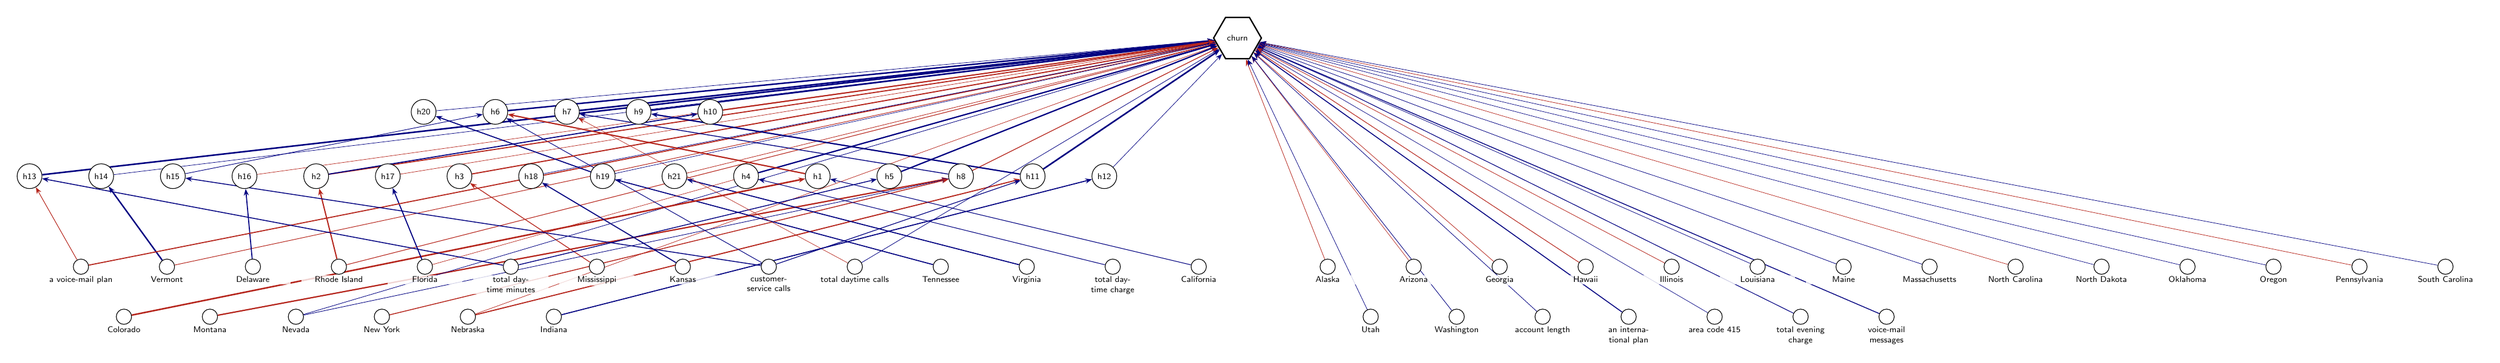
\begin{tikzpicture}[
  font=\sffamily\scriptsize, >={Stealth[length=1.4mm]},
  inp/.style={draw, circle, fill=white, minimum size=3.2mm, inner sep=0pt},
  hid/.style={draw, circle, fill=white, minimum size=5.2mm, inner sep=0.5pt, font=\sffamily\tiny},
  exitbox/.style={draw, thick, rectangle, fill=white, align=center, text width=17mm, minimum height=5mm, inner sep=1.5pt, font=\sffamily\tiny},
  sumbox/.style={draw, thick, dashed, rectangle, fill=white, align=center, text width=17mm, minimum height=5mm, inner sep=1.5pt, font=\sffamily\tiny},
  outp/.style={draw, thick, regular polygon, regular polygon sides=6, fill=white, minimum size=10mm, inner sep=0pt, font=\sffamily\tiny, align=center},
  stub/.style={draw, dashed, rounded corners=2pt, fill=white, align=center, inner sep=2pt, font=\sffamily\tiny, text width=15mm},
  inlab/.style={font=\sffamily\tiny, align=center, text width=15mm, inner sep=1pt, fill=white, fill opacity=0.8, text opacity=1},
  wpos/.style={draw=NavyBlue}, wneg/.style={draw=BrickRed}, wagg/.style={draw=black!45, line width=1.2pt},
  wmix/.style={draw=Plum},
]
\node[inp] (ninxxstatex0) at (26.1,0.0) {};
\path (ninxxstatex0.south) node[inlab, anchor=north] (labninxxstatex0) {Alaska};
\node[inp] (ninxxstatex18) at (35.1,0.0) {};
\path (ninxxstatex18.south) node[inlab, anchor=north] (labninxxstatex18) {Louisiana};
\node[inp] (ninxxstatex19) at (38.7,0.0) {};
\path (ninxxstatex19.south) node[inlab, anchor=north] (labninxxstatex19) {Massachusetts};
\node[inp] (ninxxstatex21) at (36.9,0.0) {};
\path (ninxxstatex21.south) node[inlab, anchor=north] (labninxxstatex21) {Maine};
\node[inp] (ninxxstatex25) at (10.8,0.0) {};
\path (ninxxstatex25.south) node[inlab, anchor=north] (labninxxstatex25) {Mississippi};
\node[inp] (ninxxstatex26) at (2.7,-1.05) {};
\path (ninxxstatex26.south) node[inlab, anchor=north] (labninxxstatex26) {Montana};
\node[inp] (ninxxstatex27) at (40.5,0.0) {};
\path (ninxxstatex27.south) node[inlab, anchor=north] (labninxxstatex27) {North Carolina};
\node[inp] (ninxxstatex28) at (42.3,0.0) {};
\path (ninxxstatex28.south) node[inlab, anchor=north] (labninxxstatex28) {North Dakota};
\node[inp] (ninxxstatex29) at (8.1,-1.05) {};
\path (ninxxstatex29.south) node[inlab, anchor=north] (labninxxstatex29) {Nebraska};
\node[inp] (ninxxstatex3) at (27.9,0.0) {};
\path (ninxxstatex3.south) node[inlab, anchor=north] (labninxxstatex3) {Arizona};
\node[inp] (ninxxstatex33) at (4.5,-1.05) {};
\path (ninxxstatex33.south) node[inlab, anchor=north] (labninxxstatex33) {Nevada};
\node[inp] (ninxxstatex34) at (6.3,-1.05) {};
\path (ninxxstatex34.south) node[inlab, anchor=north] (labninxxstatex34) {New York};
\node[inp] (ninxxstatex10) at (29.7,0.0) {};
\path (ninxxstatex10.south) node[inlab, anchor=north] (labninxxstatex10) {Georgia};
\node[inp] (ninxxstatex36) at (44.1,0.0) {};
\path (ninxxstatex36.south) node[inlab, anchor=north] (labninxxstatex36) {Oklahoma};
\node[inp] (ninxxstatex37) at (45.9,0.0) {};
\path (ninxxstatex37.south) node[inlab, anchor=north] (labninxxstatex37) {Oregon};
\node[inp] (ninxxstatex38) at (47.7,0.0) {};
\path (ninxxstatex38.south) node[inlab, anchor=north] (labninxxstatex38) {Pennsylvania};
\node[inp] (ninxxstatex39) at (5.4,0.0) {};
\path (ninxxstatex39.south) node[inlab, anchor=north] (labninxxstatex39) {Rhode Island};
\node[inp] (ninxxstatex4) at (23.4,0.0) {};
\path (ninxxstatex4.south) node[inlab, anchor=north] (labninxxstatex4) {California};
\node[inp] (ninxxstatex40) at (49.5,0.0) {};
\path (ninxxstatex40.south) node[inlab, anchor=north] (labninxxstatex40) {South Carolina};
\node[inp] (ninxxstatex42) at (18.0,0.0) {};
\path (ninxxstatex42.south) node[inlab, anchor=north] (labninxxstatex42) {Tennessee};
\node[inp] (ninxxstatex11) at (31.5,0.0) {};
\path (ninxxstatex11.south) node[inlab, anchor=north] (labninxxstatex11) {Hawaii};
\node[inp] (ninxxstatex44) at (27.0,-1.05) {};
\path (ninxxstatex44.south) node[inlab, anchor=north] (labninxxstatex44) {Utah};
\node[inp] (ninxxstatex45) at (19.8,0.0) {};
\path (ninxxstatex45.south) node[inlab, anchor=north] (labninxxstatex45) {Virginia};
\node[inp] (ninxxstatex46) at (1.8,0.0) {};
\path (ninxxstatex46.south) node[inlab, anchor=north] (labninxxstatex46) {Vermont};
\node[inp] (ninxxstatex47) at (28.8,-1.05) {};
\path (ninxxstatex47.south) node[inlab, anchor=north] (labninxxstatex47) {Washington};
\node[inp] (ninxxstatex5) at (0.9,-1.05) {};
\path (ninxxstatex5.south) node[inlab, anchor=north] (labninxxstatex5) {Colorado};
\node[inp] (ninxxstatex8) at (3.6,0.0) {};
\path (ninxxstatex8.south) node[inlab, anchor=north] (labninxxstatex8) {Delaware};
\node[inp] (ninxxstatex9) at (7.2,0.0) {};
\path (ninxxstatex9.south) node[inlab, anchor=north] (labninxxstatex9) {Florida};
\node[inp] (ninxxaccountxlength) at (30.6,-1.05) {};
\path (ninxxaccountxlength.south) node[inlab, anchor=north] (labninxxaccountxlength) {account length};
\node[inp] (ninxxareaxcodex415) at (34.2,-1.05) {};
\path (ninxxareaxcodex415.south) node[inlab, anchor=north] (labninxxareaxcodex415) {area code 415};
\node[inp] (ninxxinternationalxplan) at (32.4,-1.05) {};
\path (ninxxinternationalxplan.south) node[inlab, anchor=north] (labninxxinternationalxplan) {an international plan};
\node[inp] (ninxxvoicexmailxplan) at (0.0,0.0) {};
\path (ninxxvoicexmailxplan.south) node[inlab, anchor=north] (labninxxvoicexmailxplan) {a voice-mail plan};
\node[inp] (ninxxnumberxvmailxmessages) at (37.8,-1.05) {};
\path (ninxxnumberxvmailxmessages.south) node[inlab, anchor=north] (labninxxnumberxvmailxmessages) {voice-mail messages};
\node[inp] (ninxxtotalxdayxminutes) at (9.0,0.0) {};
\path (ninxxtotalxdayxminutes.south) node[inlab, anchor=north] (labninxxtotalxdayxminutes) {total daytime minutes};
\node[inp] (ninxxtotalxdayxcalls) at (16.2,0.0) {};
\path (ninxxtotalxdayxcalls.south) node[inlab, anchor=north] (labninxxtotalxdayxcalls) {total daytime calls};
\node[inp] (ninxxtotalxdayxcharge) at (21.6,0.0) {};
\path (ninxxtotalxdayxcharge.south) node[inlab, anchor=north] (labninxxtotalxdayxcharge) {total daytime charge};
\node[inp] (ninxxtotalxevexcharge) at (36.0,-1.05) {};
\path (ninxxtotalxevexcharge.south) node[inlab, anchor=north] (labninxxtotalxevexcharge) {total evening charge};
\node[inp] (ninxxstatex14) at (33.3,0.0) {};
\path (ninxxstatex14.south) node[inlab, anchor=north] (labninxxstatex14) {Illinois};
\node[inp] (ninxxnumberxcustomerxservicexcalls) at (14.4,0.0) {};
\path (ninxxnumberxcustomerxservicexcalls.south) node[inlab, anchor=north] (labninxxnumberxcustomerxservicexcalls) {customer-service calls};
\node[inp] (ninxxstatex15) at (9.9,-1.05) {};
\path (ninxxstatex15.south) node[inlab, anchor=north] (labninxxstatex15) {Indiana};
\node[inp] (ninxxstatex16) at (12.6,0.0) {};
\path (ninxxstatex16.south) node[inlab, anchor=north] (labninxxstatex16) {Kansas};
\node[outp] (n0) at (24.212,4.8) {churn};
\node[hid] (n10131) at (-1.076,1.9) {h13};
\node[hid] (n11361) at (0.424,1.9) {h14};
\node[hid] (n12374) at (1.924,1.9) {h15};
\node[hid] (n12690) at (3.424,1.9) {h16};
\node[hid] (n1295) at (4.924,1.9) {h2};
\node[hid] (n13068) at (6.424,1.9) {h17};
\node[hid] (n1390) at (7.924,1.9) {h3};
\node[hid] (n15362) at (9.424,1.9) {h18};
\node[hid] (n15490) at (10.924,1.9) {h19};
\node[hid] (n15904) at (7.174,3.25) {h20};
\node[hid] (n17102) at (12.424,1.9) {h21};
\node[hid] (n3118) at (13.924,1.9) {h4};
\node[hid] (n349) at (15.424,1.9) {h1};
\node[hid] (n4000) at (16.924,1.9) {h5};
\node[hid] (n5268) at (8.674,3.25) {h6};
\node[hid] (n5533) at (10.174,3.25) {h7};
\node[hid] (n5786) at (18.424,1.9) {h8};
\node[hid] (n6713) at (11.674,3.25) {h9};
\node[hid] (n7872) at (13.174,3.25) {h10};
\node[hid] (n9436) at (19.924,1.9) {h11};
\node[hid] (n9954) at (21.424,1.9) {h12};
\begin{scope}[on background layer]
\draw[->, wneg, line width=0.29pt] (ninxxstatex0) -- (n0);
\draw[->, wpos, line width=0.27pt] (ninxxstatex18) -- (n0);
\draw[->, wpos, line width=0.27pt] (ninxxstatex19) -- (n0);
\draw[->, wpos, line width=0.29pt] (ninxxstatex21) -- (n0);
\draw[->, wneg, line width=0.45pt] (ninxxstatex25) -- (n1390);
\draw[->, wneg, line width=0.78pt] (ninxxstatex26) -- (n5786);
\draw[->, wneg, line width=0.26pt] (ninxxstatex27) -- (n0);
\draw[->, wpos, line width=0.25pt] (ninxxstatex28) -- (n0);
\draw[->, wneg, line width=0.27pt] (ninxxstatex29) -- (n0);
\draw[->, wneg, line width=0.64pt] (ninxxstatex29) -- (n9436);
\draw[->, wneg, line width=0.25pt] (ninxxstatex3) -- (n0);
\draw[->, wpos, line width=0.30pt] (ninxxstatex33) -- (n0);
\draw[->, wpos, line width=0.31pt] (ninxxstatex33) -- (n5786);
\draw[->, wneg, line width=0.51pt] (ninxxstatex34) -- (n5786);
\draw[->, wneg, line width=0.28pt] (ninxxstatex10) -- (n0);
\draw[->, wpos, line width=0.25pt] (ninxxstatex36) -- (n0);
\draw[->, wpos, line width=0.26pt] (ninxxstatex37) -- (n0);
\draw[->, wneg, line width=0.28pt] (ninxxstatex38) -- (n0);
\draw[->, wneg, line width=0.39pt] (ninxxstatex39) -- (n0);
\draw[->, wneg, line width=0.70pt] (ninxxstatex39) -- (n1295);
\draw[->, wpos, line width=0.39pt] (ninxxstatex4) -- (n349);
\draw[->, wpos, line width=0.27pt] (ninxxstatex40) -- (n0);
\draw[->, wpos, line width=0.59pt] (ninxxstatex42) -- (n15490);
\draw[->, wneg, line width=0.37pt] (ninxxstatex11) -- (n0);
\draw[->, wpos, line width=0.27pt] (ninxxstatex44) -- (n0);
\draw[->, wpos, line width=0.60pt] (ninxxstatex45) -- (n17102);
\draw[->, wneg, line width=0.36pt] (ninxxstatex46) -- (n0);
\draw[->, wpos, line width=0.83pt] (ninxxstatex46) -- (n11361);
\draw[->, wpos, line width=0.31pt] (ninxxstatex47) -- (n0);
\draw[->, wneg, line width=0.90pt] (ninxxstatex5) -- (n349);
\draw[->, wpos, line width=0.60pt] (ninxxstatex8) -- (n12690);
\draw[->, wneg, line width=0.26pt] (ninxxstatex9) -- (n0);
\draw[->, wpos, line width=0.61pt] (ninxxstatex9) -- (n13068);
\draw[->, wpos, line width=0.29pt] (ninxxaccountxlength) -- (n0);
\draw[->, wpos, line width=0.25pt] (ninxxareaxcodex415) -- (n0);
\draw[->, wpos, line width=0.53pt] (ninxxinternationalxplan) -- (n0);
\draw[->, wneg, line width=0.62pt] (ninxxvoicexmailxplan) -- (n0);
\draw[->, wneg, line width=0.37pt] (ninxxvoicexmailxplan) -- (n10131);
\draw[->, wpos, line width=0.49pt] (ninxxnumberxvmailxmessages) -- (n0);
\draw[->, wpos, line width=0.53pt] (ninxxtotalxdayxminutes) -- (n10131);
\draw[->, wpos, line width=0.50pt] (ninxxtotalxdayxminutes) -- (n4000);
\draw[->, wpos, line width=0.29pt] (ninxxtotalxdayxcalls) -- (n0);
\draw[->, wneg, line width=0.25pt] (ninxxtotalxdayxcalls) -- (n5533);
\draw[->, wpos, line width=0.38pt] (ninxxtotalxdayxcharge) -- (n3118);
\draw[->, wpos, line width=0.39pt] (ninxxtotalxevexcharge) -- (n0);
\draw[->, wneg, line width=0.29pt] (ninxxstatex14) -- (n0);
\draw[->, wpos, line width=0.51pt] (ninxxnumberxcustomerxservicexcalls) -- (n12374);
\draw[->, wpos, line width=0.36pt] (ninxxnumberxcustomerxservicexcalls) -- (n5268);
\draw[->, wpos, line width=0.43pt] (ninxxnumberxcustomerxservicexcalls) -- (n9436);
\draw[->, wpos, line width=0.60pt] (ninxxstatex15) -- (n9954);
\draw[->, wpos, line width=0.60pt] (ninxxstatex16) -- (n15362);
\draw[->, wpos, line width=0.91pt] (n10131) -- (n0);
\draw[->, wpos, line width=0.27pt] (n11361) -- (n0);
\draw[->, wpos, line width=0.34pt] (n12374) -- (n5268);
\draw[->, wneg, line width=0.26pt] (n12690) -- (n0);
\draw[->, wneg, line width=0.64pt] (n1295) -- (n0);
\draw[->, wpos, line width=0.61pt] (n1295) -- (n7872);
\draw[->, wneg, line width=0.26pt] (n13068) -- (n0);
\draw[->, wneg, line width=0.66pt] (n1390) -- (n0);
\draw[->, wpos, line width=0.27pt] (n15362) -- (n0);
\draw[->, wpos, line width=0.26pt] (n15490) -- (n0);
\draw[->, wpos, line width=0.60pt] (n15490) -- (n15904);
\draw[->, wpos, line width=0.27pt] (n15904) -- (n0);
\draw[->, wneg, line width=0.30pt] (n17102) -- (n0);
\draw[->, wpos, line width=0.77pt] (n3118) -- (n0);
\draw[->, wneg, line width=0.74pt] (n349) -- (n5268);
\draw[->, wpos, line width=0.77pt] (n4000) -- (n0);
\draw[->, wpos, line width=0.85pt] (n5268) -- (n0);
\draw[->, wpos, line width=0.94pt] (n5533) -- (n0);
\draw[->, wneg, line width=0.44pt] (n5786) -- (n0);
\draw[->, wpos, line width=0.48pt] (n5786) -- (n5533);
\draw[->, wpos, line width=0.86pt] (n6713) -- (n0);
\draw[->, wneg, line width=0.69pt] (n7872) -- (n0);
\draw[->, wpos, line width=0.91pt] (n9436) -- (n0);
\draw[->, wpos, line width=0.77pt] (n9436) -- (n6713);
\draw[->, wpos, line width=0.27pt] (n9954) -- (n0);
\end{scope}
\end{tikzpicture}}%
\caption{The network as trained, before any explanation, in full. Blue: positive weight (raises the score); red: negative weight (lowers it); thicker: larger weight. Orange outline and up arrow: raises the final prediction; teal and down arrow: lowers it; grey and double arrow: depends. Not used (no connection): Alabama, Iowa, Idaho, Kentucky, Arkansas, Maryland, Michigan, Minnesota, Missouri, New Hampshire, New Jersey, New Mexico, Ohio, South Dakota, Texas, Wisconsin, West Virginia, Wyoming, Connecticut, Washington DC, area code 408, area code 510, total evening minutes, total evening calls, total night-time minutes, total night-time calls, total night-time charge, total international minutes, total international calls, total international charge.}
\label{fig:churn100s4c3:raw}
\end{figure}
\end{landscape}
\end{drafted}
\clearpage
\end{document}
